\documentclass[]{report}
\usepackage[utf8]{inputenc}
\usepackage{amssymb}
\usepackage{amsmath}
\usepackage{booktabs}
\usepackage{graphicx}
\graphicspath{{images/}}
\usepackage{caption}
\usepackage{subcaption}
\usepackage{braket}
\usepackage{changepage}
\usepackage[a4paper,width=150mm,top=0.75in,bottom=0.75in]{geometry}
\usepackage{mwe}
\usepackage{float}
\usepackage[font=footnotesize,labelfont=bf]{caption}
\usepackage{bbold}
\usepackage{framed}
\usepackage{sidecap}
\usepackage{hyperref}
\usepackage{setspace}
\usepackage{notoccite}
\usepackage{cleveref}
\usepackage{physics}
\usepackage{siunitx}
% \usepackage[nottoc,numbib]{tocbibind}
\usepackage[style=ieee, citestyle=numeric-comp, backend=biber]{biblatex}

\setlength{\parindent}{0pt}
\renewcommand{\figurename}{Fig.}
\newtheorem{theorem}{Theorem}

\title{Towards Accurate DeepMD Potentials for Aqueous Interfaces}
\author{Christian Loer Llemit\\[1cm]{Supervisors:}\\{\small  Ali
Hassanali}\\{\small Cesare Malosso}\\{\small Edward Donkor} }
\date{August 2024}

\addbibresource{references.bib}

\begin{document}

\maketitle
\pagenumbering{arabic}
%\chapter*{Abstract}

\chapter*{Acknowledgement}
\addcontentsline{toc}{chapter}{Acknowledgement}

I would like to thank Ali Hassanali, my supervisor, for all the guidance that made the completion of the thesis possible. I thanked him for rendering his valuable time in giving constructive criticism and to instill in my mind to always ask questions and examine all possible solutions to unanswered problems. I thanked Cesare Malosso, my co-supervisor, for guiding me in preparing codes, for orienting me on how the code works, and for his feedbacks. I also thanked Edward Donkor, my co-supervisor, for giving me some of his codes and for his  feedbacks. I thanked the atomistic simulations group for grilling my presentation for which I improved a lot.

I thanked all the professors for rendering their time and sharing their expertise to future prospective full-fledged scientists. I  thanked the library staffs for all the assistance. I thanked my fellow classmates for the fruitful discussions.

I want to thank Alexandra Santos and Darwin Putungan for pushing me to apply the post-graduate diploma program. I want to express  gratitude to my family who supported me all throughout my journey.

Lastyl, I extend my gratitude  to ICTP for this wonderful institution that helps students from developing countries.

\tableofcontents

\setstretch{1.5}

\chapter*{Abstract}
\addcontentsline{toc}{chapter}{Abstract}

This thesis explores the challenges and issues in modelling the many-body potential energy surface
for liquid water interfaces by means of developing deep neural network potential  scheme for molecular dynamics simulations (DPMD), as implemented in DeePMD-kit. We focus on modelling  neat water interfaces by training the datasets of bulk and bulk+interface systems with Density Functional Theory (DFT) level of accuracy and linear scale efficiency of empirical force fields. In addition, DPMD can be parallelized due to its local decomposition and  near-neighbor dependence of  atomic energies. The generated deep neural network potential (NNP) was assessed according to its predictability in obtaining relevant system properties such as mass density, surface tension, and dipole orientation. Due to numerical instabilities using SCAN functional for interfaces, we used instead a similar  but accurate and numerically efficient regularized-restored r$^2$SCAN functional in labelling the datasets. Neural network potential trained on only bulk
systems did not perform well when used on trajectories containing interfaces. Adding interface dataset to the training
did improve the prediction  of macroscopic properties, implying that surface defects
play a role in surface properties of water. In addition, the bulk+interface trained NNP have the same accuracy as the reference NNP used but with a smaller  training dataset. All the models  fail to describe microscopic properties such as dipole orientation at the surface but still obtain good macroscopic properties such as surface tension for the bulk+interface trained NNP.  Finite size effects  and  long-range electrostatic interactions might play a role in obtaining  discrepancies at the microscopic level.

\chapter{Introduction}

\section{Objectives}

Describe importance of analyzing interfaces. Surface tension of different
solutes.

\begin{itemize}
    \item To develop accurate and transferrable DeepNN potentials for
          interfaces
    \item To explore the quality of the training data set in improving the
          description of water interfaces.
    \item To understand reliability of the current architecture of DeepMD in
          dealing with interfaces.

\end{itemize}
\chapter{Theory}
\chapter{Methodology}
Typical procedure in doing deep neural MD simulation is as follows:

\begin{itemize}
    \item \emph{Data Exploration}. Before training a model, one needs to supply
          first inputs such as	atom type, the simulation box, atom
          coordinates, etc.	 Initial trajectories were generated
          using Molecular Dynamics implemented in
          LAMMPS \cite{LAMMPS}. The pair potential used is based on the
          previously
          trained deep neural network potential (NNP) generated by
          Sanchez-Burgos et
          al.
          \cite{sanchez2023deep}.

          For the MD simulation, a system size of 192 water molecules was used
          for both
          the bulk and interface systems, as shown in Figure
          \ref{fig:cryst_sctruct}. The
          temperature was varied from 300 K to 600 K. The simulation profile of
          the bulk
          system is as follows: NPT ensemble at 1 bar for 2 ns, and a ramp from
          1 bar to
          10,000 bar for 10 ns. For the interface system, the simulation was
          done in
          NVT
          ensemble for 10 ns and the box size was based on the average length
          of the
          corresponding bulk system at a given temperature and at 1 bar. Vacuum
          was
          introduced as to create a total length of 50 \r{A} in the direction
          normal to
          the interface. For both systems,
          Nosé-Hoover thermostat  with a
          relaxation time of 20 fs, and  Nosé-Hoover barostat with a relaxation
          time of 200 fs were
          applied. The equations of motion were integrated
          using the time-reversible measure-preserving Verlet and rRESPA
          integrators derived by Tuckerman et al. \cite{Tuckerman2006} with a
          simulation step of 0.2 fs.

          \begin{figure}[tbhp]
              \centering
              \begin{subfigure}{0.42\textwidth}
                  \centering
                  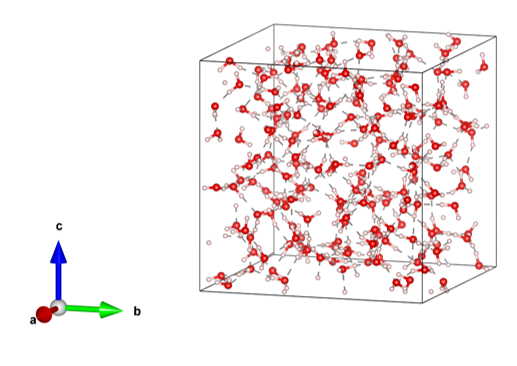
\includegraphics[width=0.75\textwidth]{bulk}
                  \caption{}
                  % \label{fig:}
              \end{subfigure}
              % \hfill
              \begin{subfigure}{0.42\textwidth}
                  \centering
                  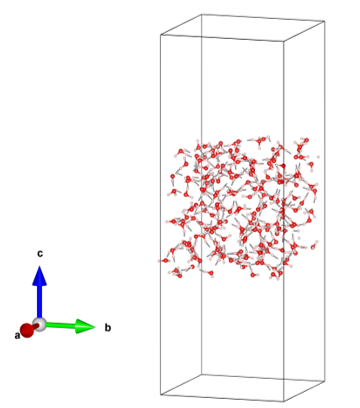
\includegraphics[width=0.75\textwidth]{interface}
                  \caption{}
                  % \label{fig:}
              \end{subfigure}
              \hfill
              \caption{Typical configurations for (a) bulk and (b) interface
                  systems.}
              \label{fig:cryst_sctruct}
          \end{figure}

    \item \emph{Data Labeling}.
          The trajectories were then labeled with their energy, force, and
          pressure
          tensor using Density Functional Theory (DFT) implemented in Quantum
          Espresso
          \cite{QE-2009,QE-2017,QE-2020}. Strongly Constrained and
          Appropriately
          Normed
          (SCAN) exchange-correlation functional is widely used in the study of
          water
          systems due to its great predictability in describing hydrogen bonds
          and
          van
          der Waals interactions \cite{sun2015strongly, chen2017ab}. However,
          for
          this
          study, the SCAN functional tends to be numerically unstable when
          implemented
          to systems with interfaces. Instead, this study tried to use a
          similar but accurate
          and
          numerically efficient r$^2$SCAN meta-generalized gradient
          approximation
          \cite{Furness2020}. Optimized Norm-Conserving Vanderbilt
          pseudopotentials
          \cite{hamann2013optimized} were used with energy cutoff of 130 Ry and
          scf
          convergence threshold of \num{1e-6} Ry.

    \item \emph{Training}. The labeled frames were then feed into DeePMD-kit
          code
          \cite{wang2018deepmd,zeng2023deepmd,lu2021,zhang2018end} for the
          training
          of
          deep neural network potentials. A total of 1200 original bulk frames
          and 1000 original
          interface
          frames were used as training data. The training follows a typical
          two-neutral
          network architecture. First, atomic configurations are processed by
          the
          embedding network of three layers consisting of 25, 50 and 100
          neurons
          each.
          The embedding follows the two-body smooth-edition scheme
          \cite{zhang2018end}
          that conserves radial and angular information within the cutoff
          radius of 6
          \r{A}. A switching function was applied for atoms beyond 5.5 \r{A} to
          ensure
          smooth cutoff.	Then, the atomic descriptors are build and
          given as
          input to a
          fitting network of three layers of 250 neurons each that outputs a
          scalar
          quantity such as energy. The parameters of the neural network are
          set
          during
          the training procedure by minimizing	loss function based on the mean
          squared
          error on the total energy and atomic forces predicted
          by the network with respect to the reference data. The minimization
          started with a large prefactor on the forces and ended with equal
          prefactors
          for both forces and energies.    The iterative
          minimization
          was performed with a total of 3 million batches and a learning rate
          that
          exponentially decay from \num{1e-3} to \num{3.5e-8}. Once the
          training is finished, the trained neural network will be  ``freezed''
          or dumped into a protobuf(.pb) file that can be used as a pair
          potential during MD simulation.

    \item \emph{Testing}. The neural network potential was tested by
          comparing results predicted by the NN potential with	  the results
          of DFT
          calculation on the validation datasets.

    \item \emph{Run MD}. Once the NN model is good, one can perform molecular
          dynamics simulations using the trained neural   network potential to
          predict
          system's properties of interest.

    \item \emph{Check Deviation}. It is possible that during stochastic
          gradient descent runs, the NN model reached a different local minima.
          Hence,
          the common procedure is to train multiple similar models but
          different
          initialization by providing a  random seed. These models will be used
          to run MD simulations and deviations among these models will then be
          compared. Larger deviation for structure properties (default is the
          atomic
          force) means less accuracy of the models. Using this criterion, a few
          trajectories whose max force standard deviation is within a lower and
          higher
          threshold of 0.8 \unit{eV/\angstrom} and 1.5	\unit{eV/\angstrom},
          respectively,
          will be selected and put into the next iteration. Each iteration will
          execute data labeling  and  the new data will be put together with
          initial data
          and data generated in previous iterations for the training. This is
          called active learning. For this work, five iterations were applied
          on
          the bulk
          systems with a total training data of 6080 frames.

    \item \emph{Obtain relevant properties}. Once the MD
          simulation is
          finished, one can compute properties of the system such as density,
          surface
          tension, and dipole orientation.	    The surface tension can be
          calculated according to Kirkwood-Buff
          equation
          \cite{kirkwood1949} given by

          \begin{equation}
              \gamma = \frac{L_z}{2} \left[ \expval{P_{zz}} -\frac{1}{2} \left(
                  \expval{P_{xx}} + \expval{P_{yy}} \right) \right]
              \label{eq:surf_tens}
          \end{equation}

          where $\expval{P_{ij}}$ is the $ij$th element of the pressure tensor,
          and $L_z$ is the total length of the box size in the direction normal
          to the
          surface.

\end{itemize}

\chapter{Results and Discussion}

\section{SCAN vs. r$^2$SCAN functional}
In order to do deep neural network training, one must label the dataset first
using
DFT. Implementing DFT calculations requires choosing appropriate parameters
such as exchange-correlation functional. Water is a delicate molecule that is
sensitive to the  complex competition between attractive interactions (e.g.
hydrogen bond, covalent bond, and van der Waals) that brings order and thermal
fluctuations that brings disorder to the system. A lot of work has attempted to
describe this delicate nature of water. One promising functional is the
Strongly Constrained and Appropriately Normed (SCAN)  density
functional
which is  a nonempirical semilocal meta-GGA functional that satisfies
all
known possible 17 exact constraints and  appropriately normed on systems for
which semilocal functional can be exact or extremely accurate
~\cite{sun2015strongly}.  SCAN is not fitted to any bonded system, but it
predicts certain bonding properties very well such as  atomization
energies, weak-interaction binding energies, and lattice
constants of solids, but not the energy barriers to chemical
reactions. It was shown that SCAN accurately describes covalent bonds, hydrogen
bonds, and van der Waals interactions that plays important role in the
structure and dynamics of liquid water~\cite{chen2017ab}. It is one of the
functionals that predicts ice as less dense than liquid water under standard
conditions. Unfortunately,
imposing rigid constraints can cause numerical instabilities for which we have
observed when applying SCAN for systems with interfaces. Instead, this study
used a similar but accurate and numerically efficient regularized-restored
r$^2$SCAN
meta-generalized gradient
approximation \cite{Furness2020}. r$^2$SCAN functional is based on the
previously proposed rSCAN functional that regularizes or relaxes some of the
constraints of SCAN in order to improve
numerical performance \cite{bartok2019}. r$^2$SCAN functional restores again
the constraints but with more consistent error in grid density,
requiring smaller
grids to
achieve good accuracy.

We performed a comparison between SCAN	and r$^2$SCAN exchange-correlation
functional to determine the extent of the discrepancy of the two functionals.
Figures~\ref{fig:scan_r2scan_E} and~\ref{fig:scan_r2scan_F}
shows that the total relative energy and atomic forces are in good agreement
between the two functionals. The computed root mean square error of the two
forces was
0.048 \unit{eV/\angstrom}, which is on the same magnitude as typical
validation
errors
on ML models. See Figure~\ref{fig:scan_r2scan_F_dist} for the distribution
plot of the error in forces.  Convergence tests were conducted
to determine the appropriate
energy cut-offs for the DFT calculations. As shown in
Figures~\ref{fig:conv_scan} and \ref{fig:conv_r2scan}, a  cutoff of 130 Ry  is
adequate to have convergence on  energy, force, and pressure for both the SCAN
and r$^2$SCAN functional. This is also consistent to what Chen et al.
\cite{chen2017ab} used in
their modelling of water.
\begin{figure}[tbhp]
	\centering
	\begin{subfigure}{0.48\textwidth}
		\centering

		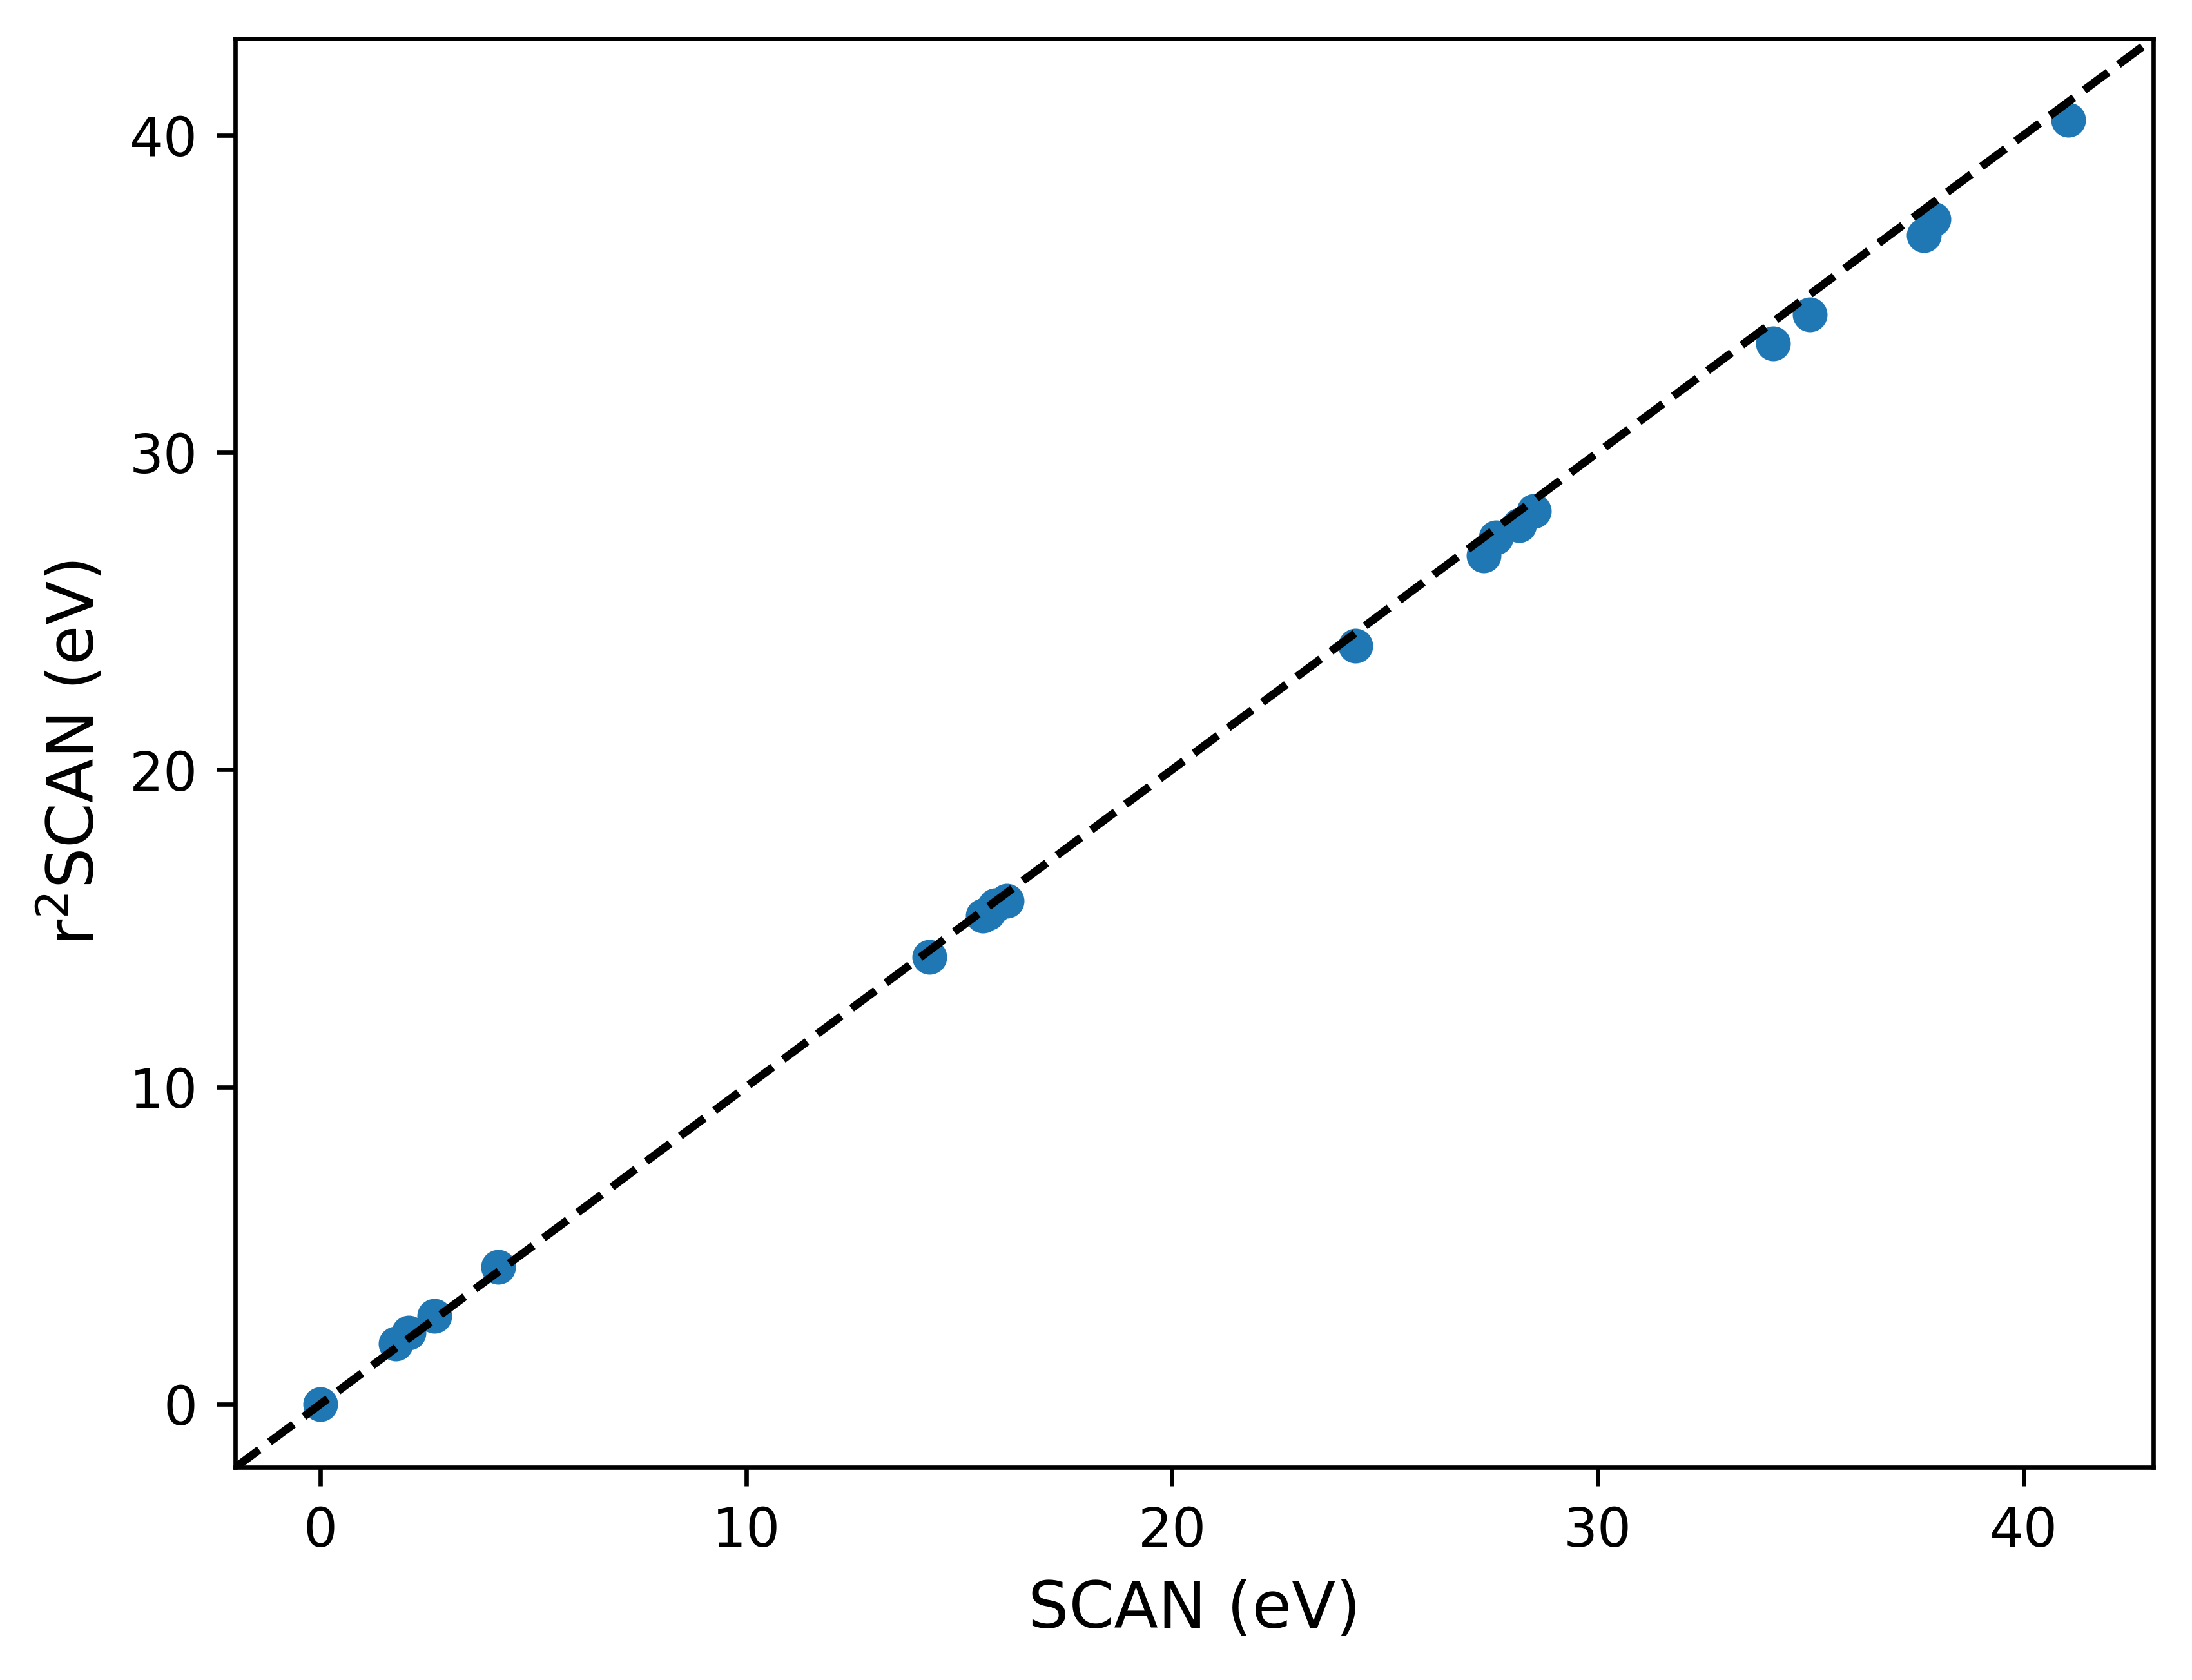
\includegraphics[width=0.9\textwidth]{images/scan_vs_r2scan/energy_compare.png}
		\caption{Relative Total Energy Comparison}
		\label{fig:scan_r2scan_E}
	\end{subfigure}
	\hfill
	\begin{subfigure}{0.48\textwidth}
		\centering

		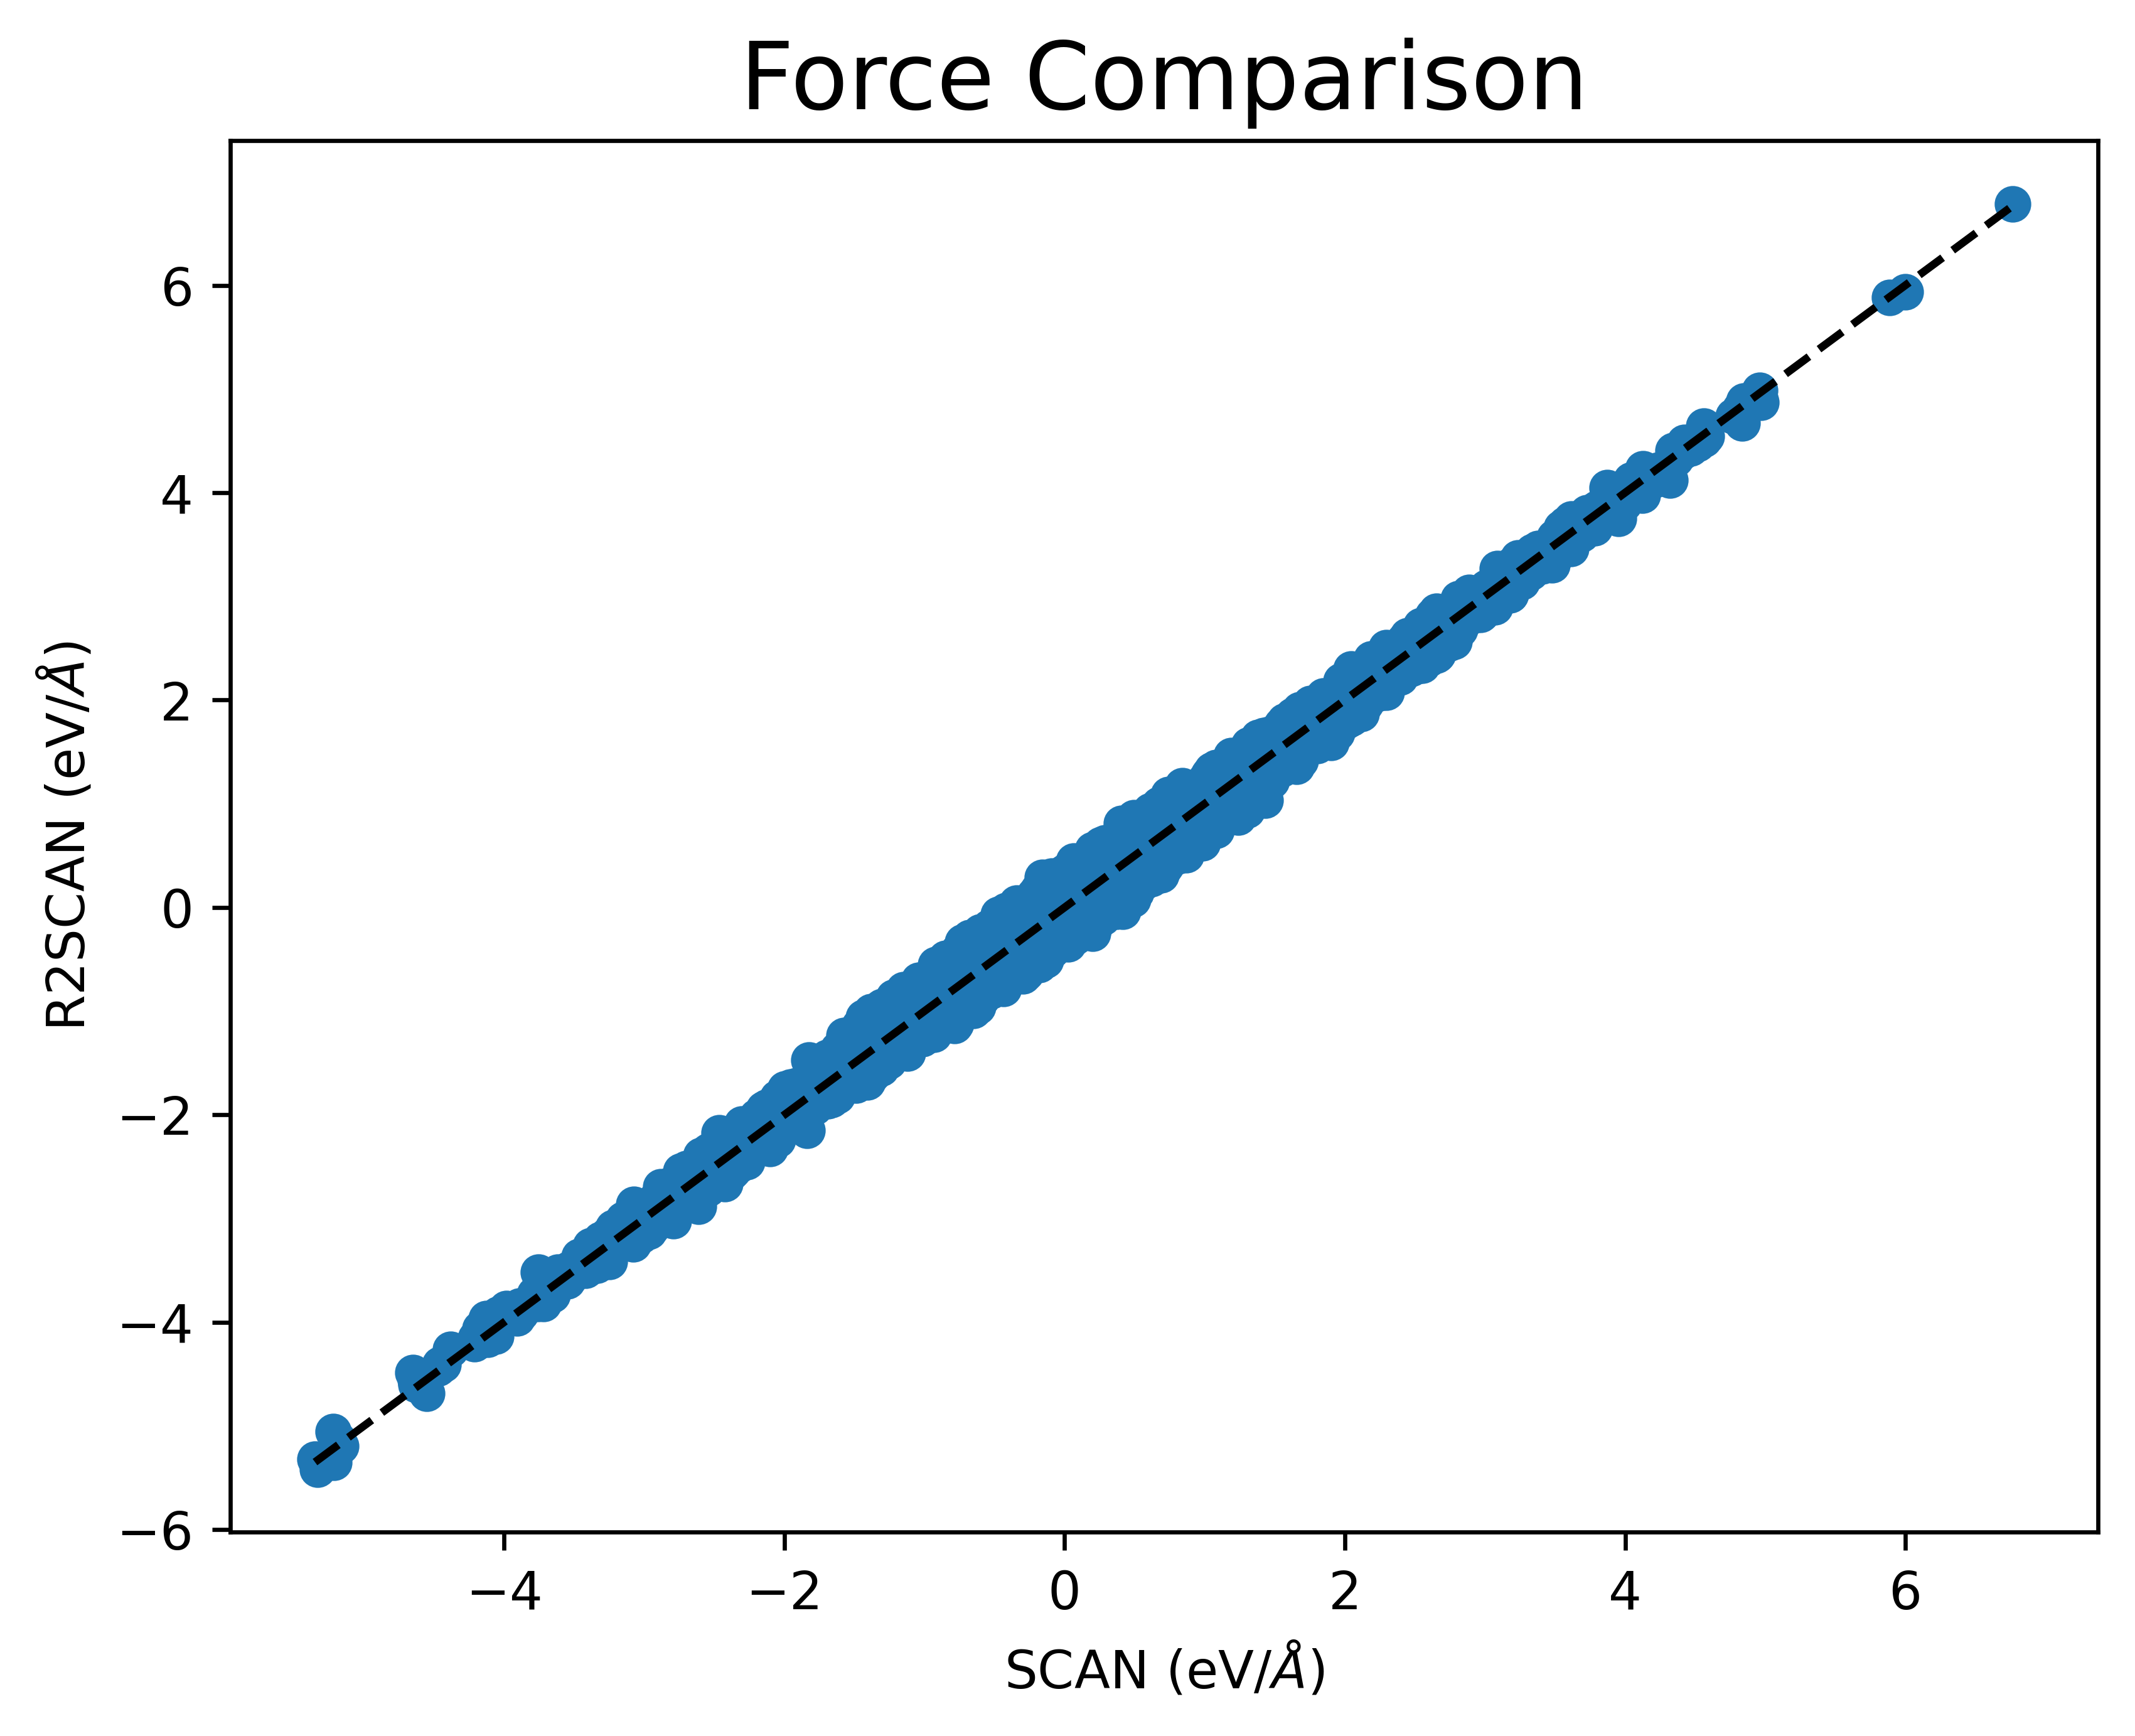
\includegraphics[width=0.9\textwidth]{images/scan_vs_r2scan/force_compare.png}
		\caption{Atomic Force Comparison}
		\label{fig:scan_r2scan_F}
	\end{subfigure}

	\caption{Correlation of  (a) relative total energy and (b) atomic force
		between 		the		SCAN and
		r$^2$SCAN functional. The relative total energy was shifted to
		the lowest energy of each corresponding functional. The
		diagonal line shows the
		perfect
		agreement between
		the two functionals.}
	\label{fig:scan_r2scan}
\end{figure}

\section{Neural Network Performance}
To check the quality of deep NN models, model deviation was calculated for the
four identical models but different initialization parameters. For each
new configuration that is explored during MD run, these models
generate an ensemble of predictions. For each configuration,
the model deviation is defined as the maximum standard deviation of the
predicted atomic forces \cite{zhang2019active,zeng2023deepmd}.  Small deviation means the model has learned the given data; otherwise, the given configuration was not covered, and the training data needs to be expanded. Note that  only the  first
model was used as pair potential during MD run to dump trajectories and
pressures during the course of simulation. When the bulk trained NNP was
used as potential for interfacial systems, the max deviation on forces has much
error, as shown in Figure~\ref{fig:dev_bulk}, implying that NNP models gave
significant differing values on forces for
a given trajectory. This is expected since the bulk trained NNP cannot
capture features associated with surfaces. During training, the NNP models may
have different minimized loss function. On the other hand,
Figure~\ref{fig:dev_bulk_interface} shows that the error is greatly reduced
when bulk+interface trained NNP was used in simulation of interfacial systems.

\begin{figure}[tbhp]
	\centering
	\begin{subfigure}{0.48\textwidth}
		\centering

		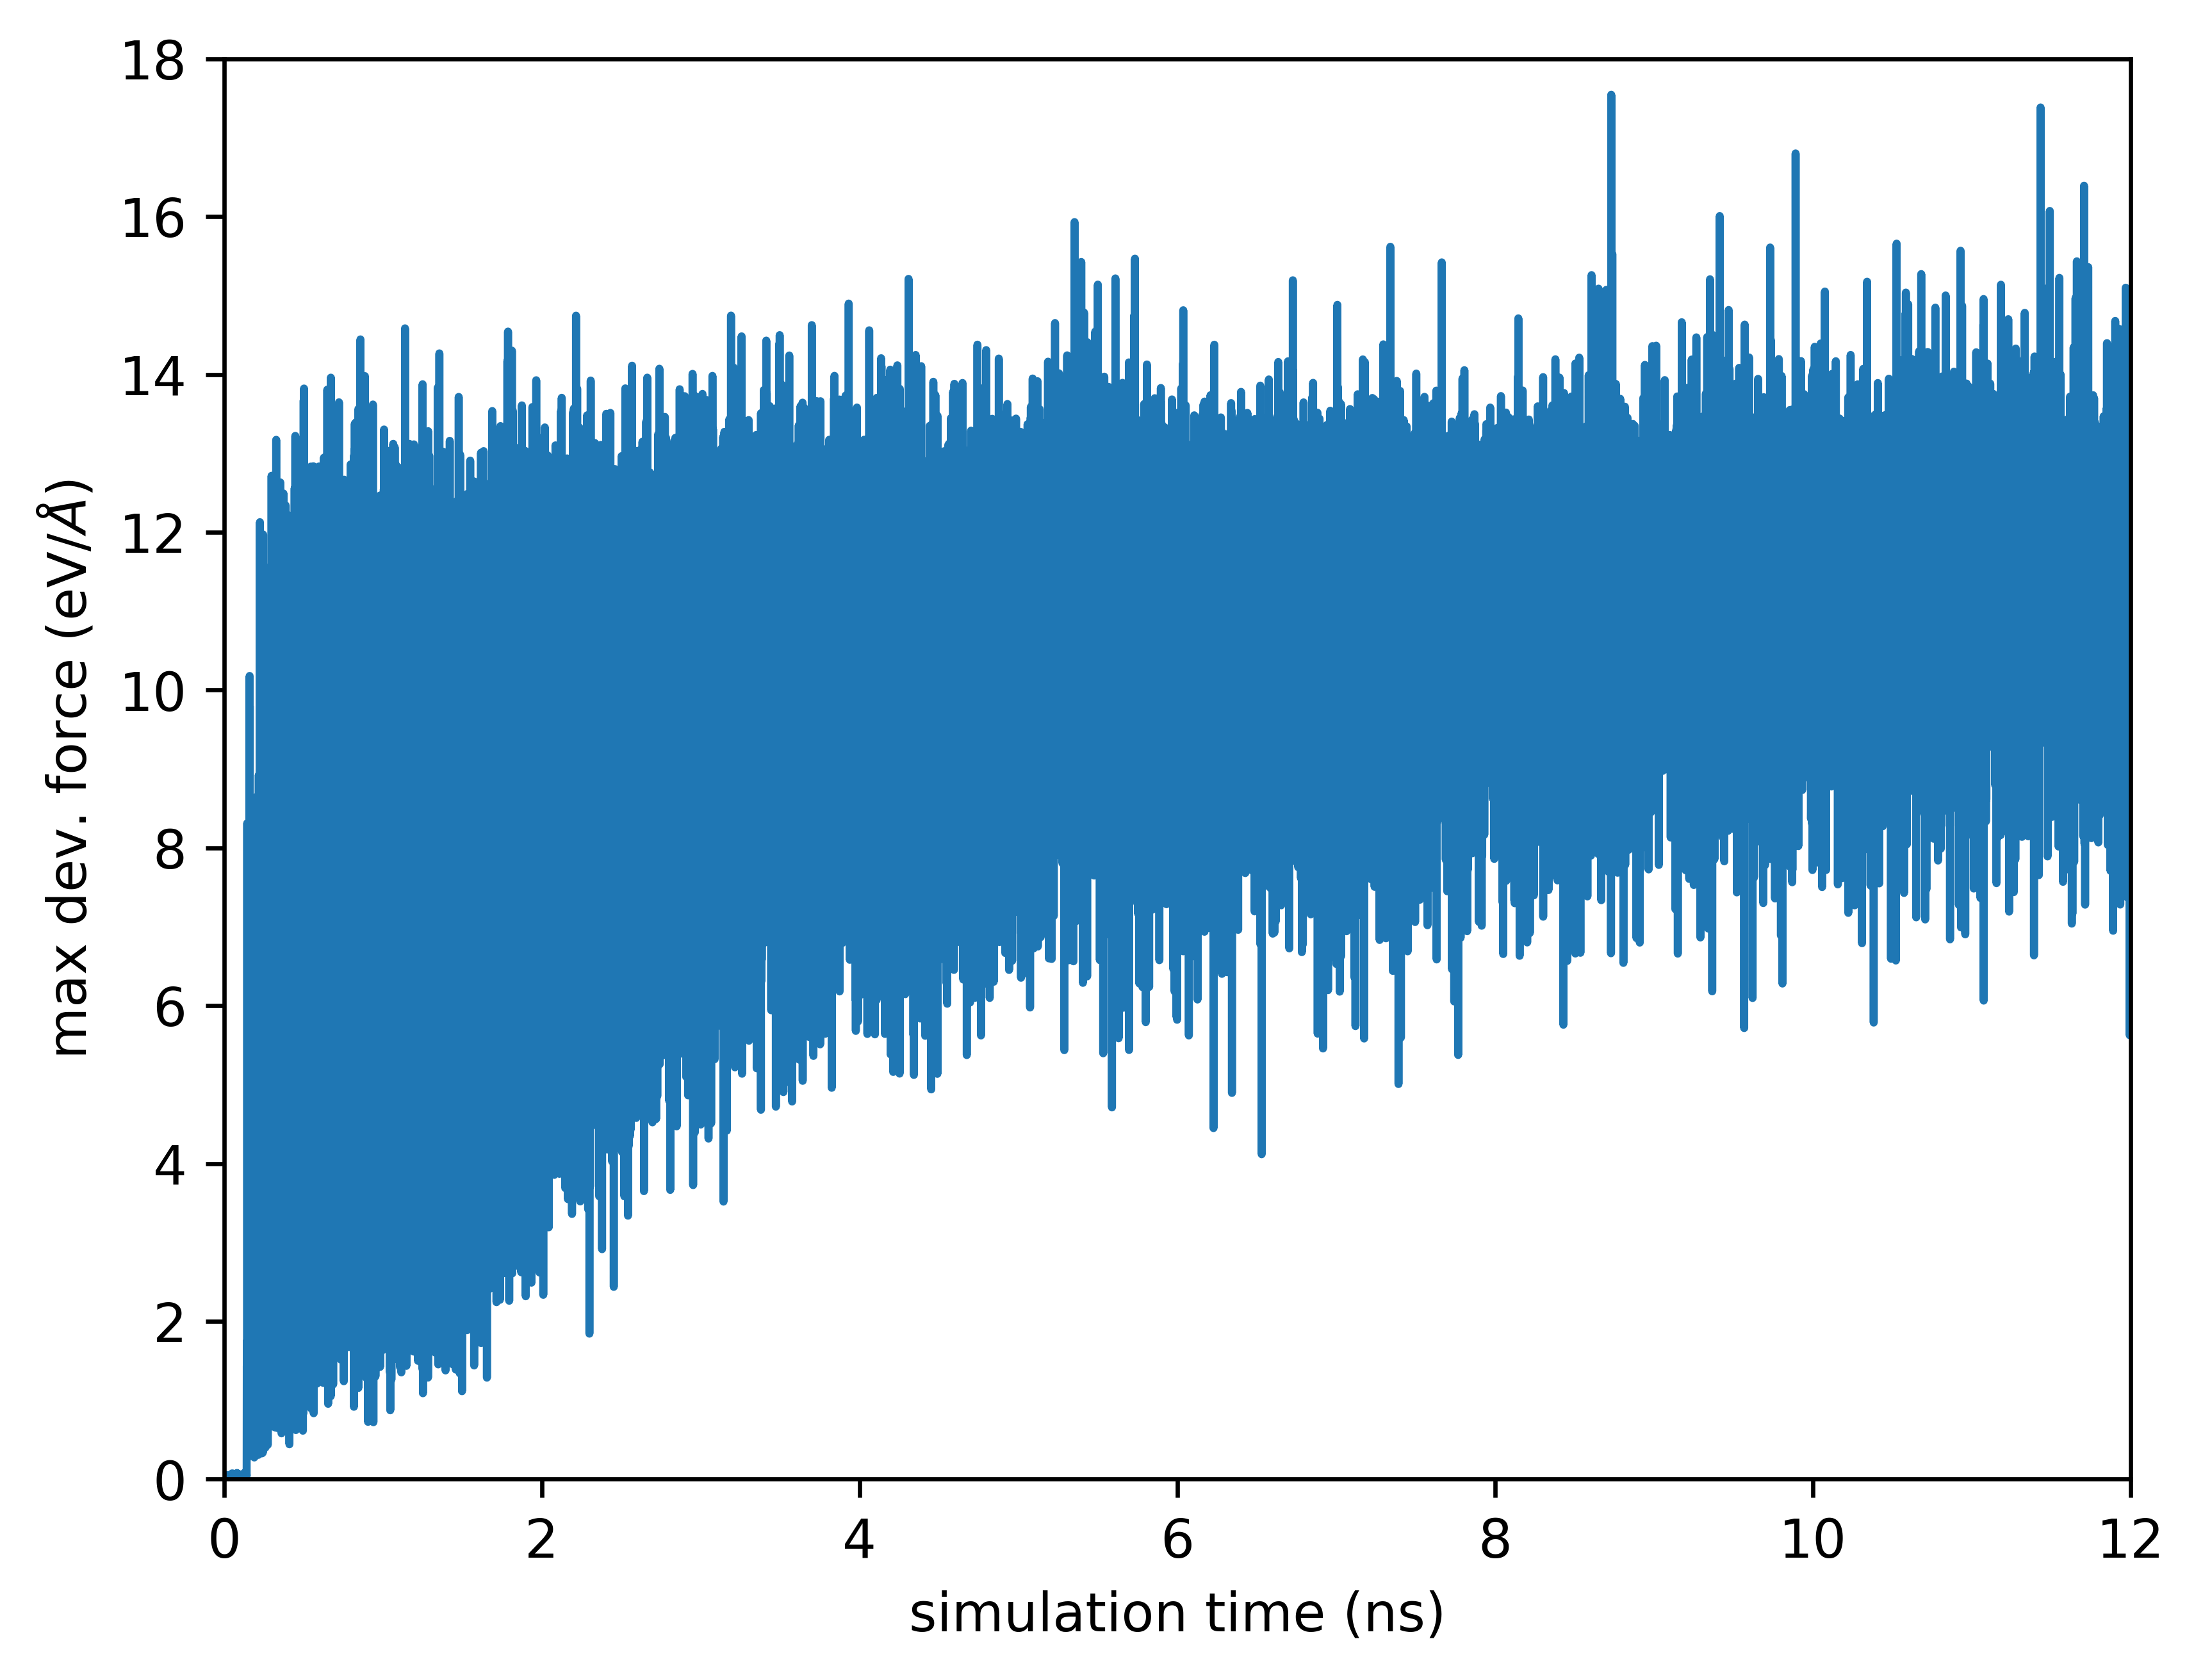
\includegraphics[width=0.9\textwidth]{images/deviation_bulk}
		\caption{Bulk trained NNP}
		\label{fig:dev_bulk}
	\end{subfigure}
	\hfill
	\begin{subfigure}{0.48\textwidth}
		\centering

		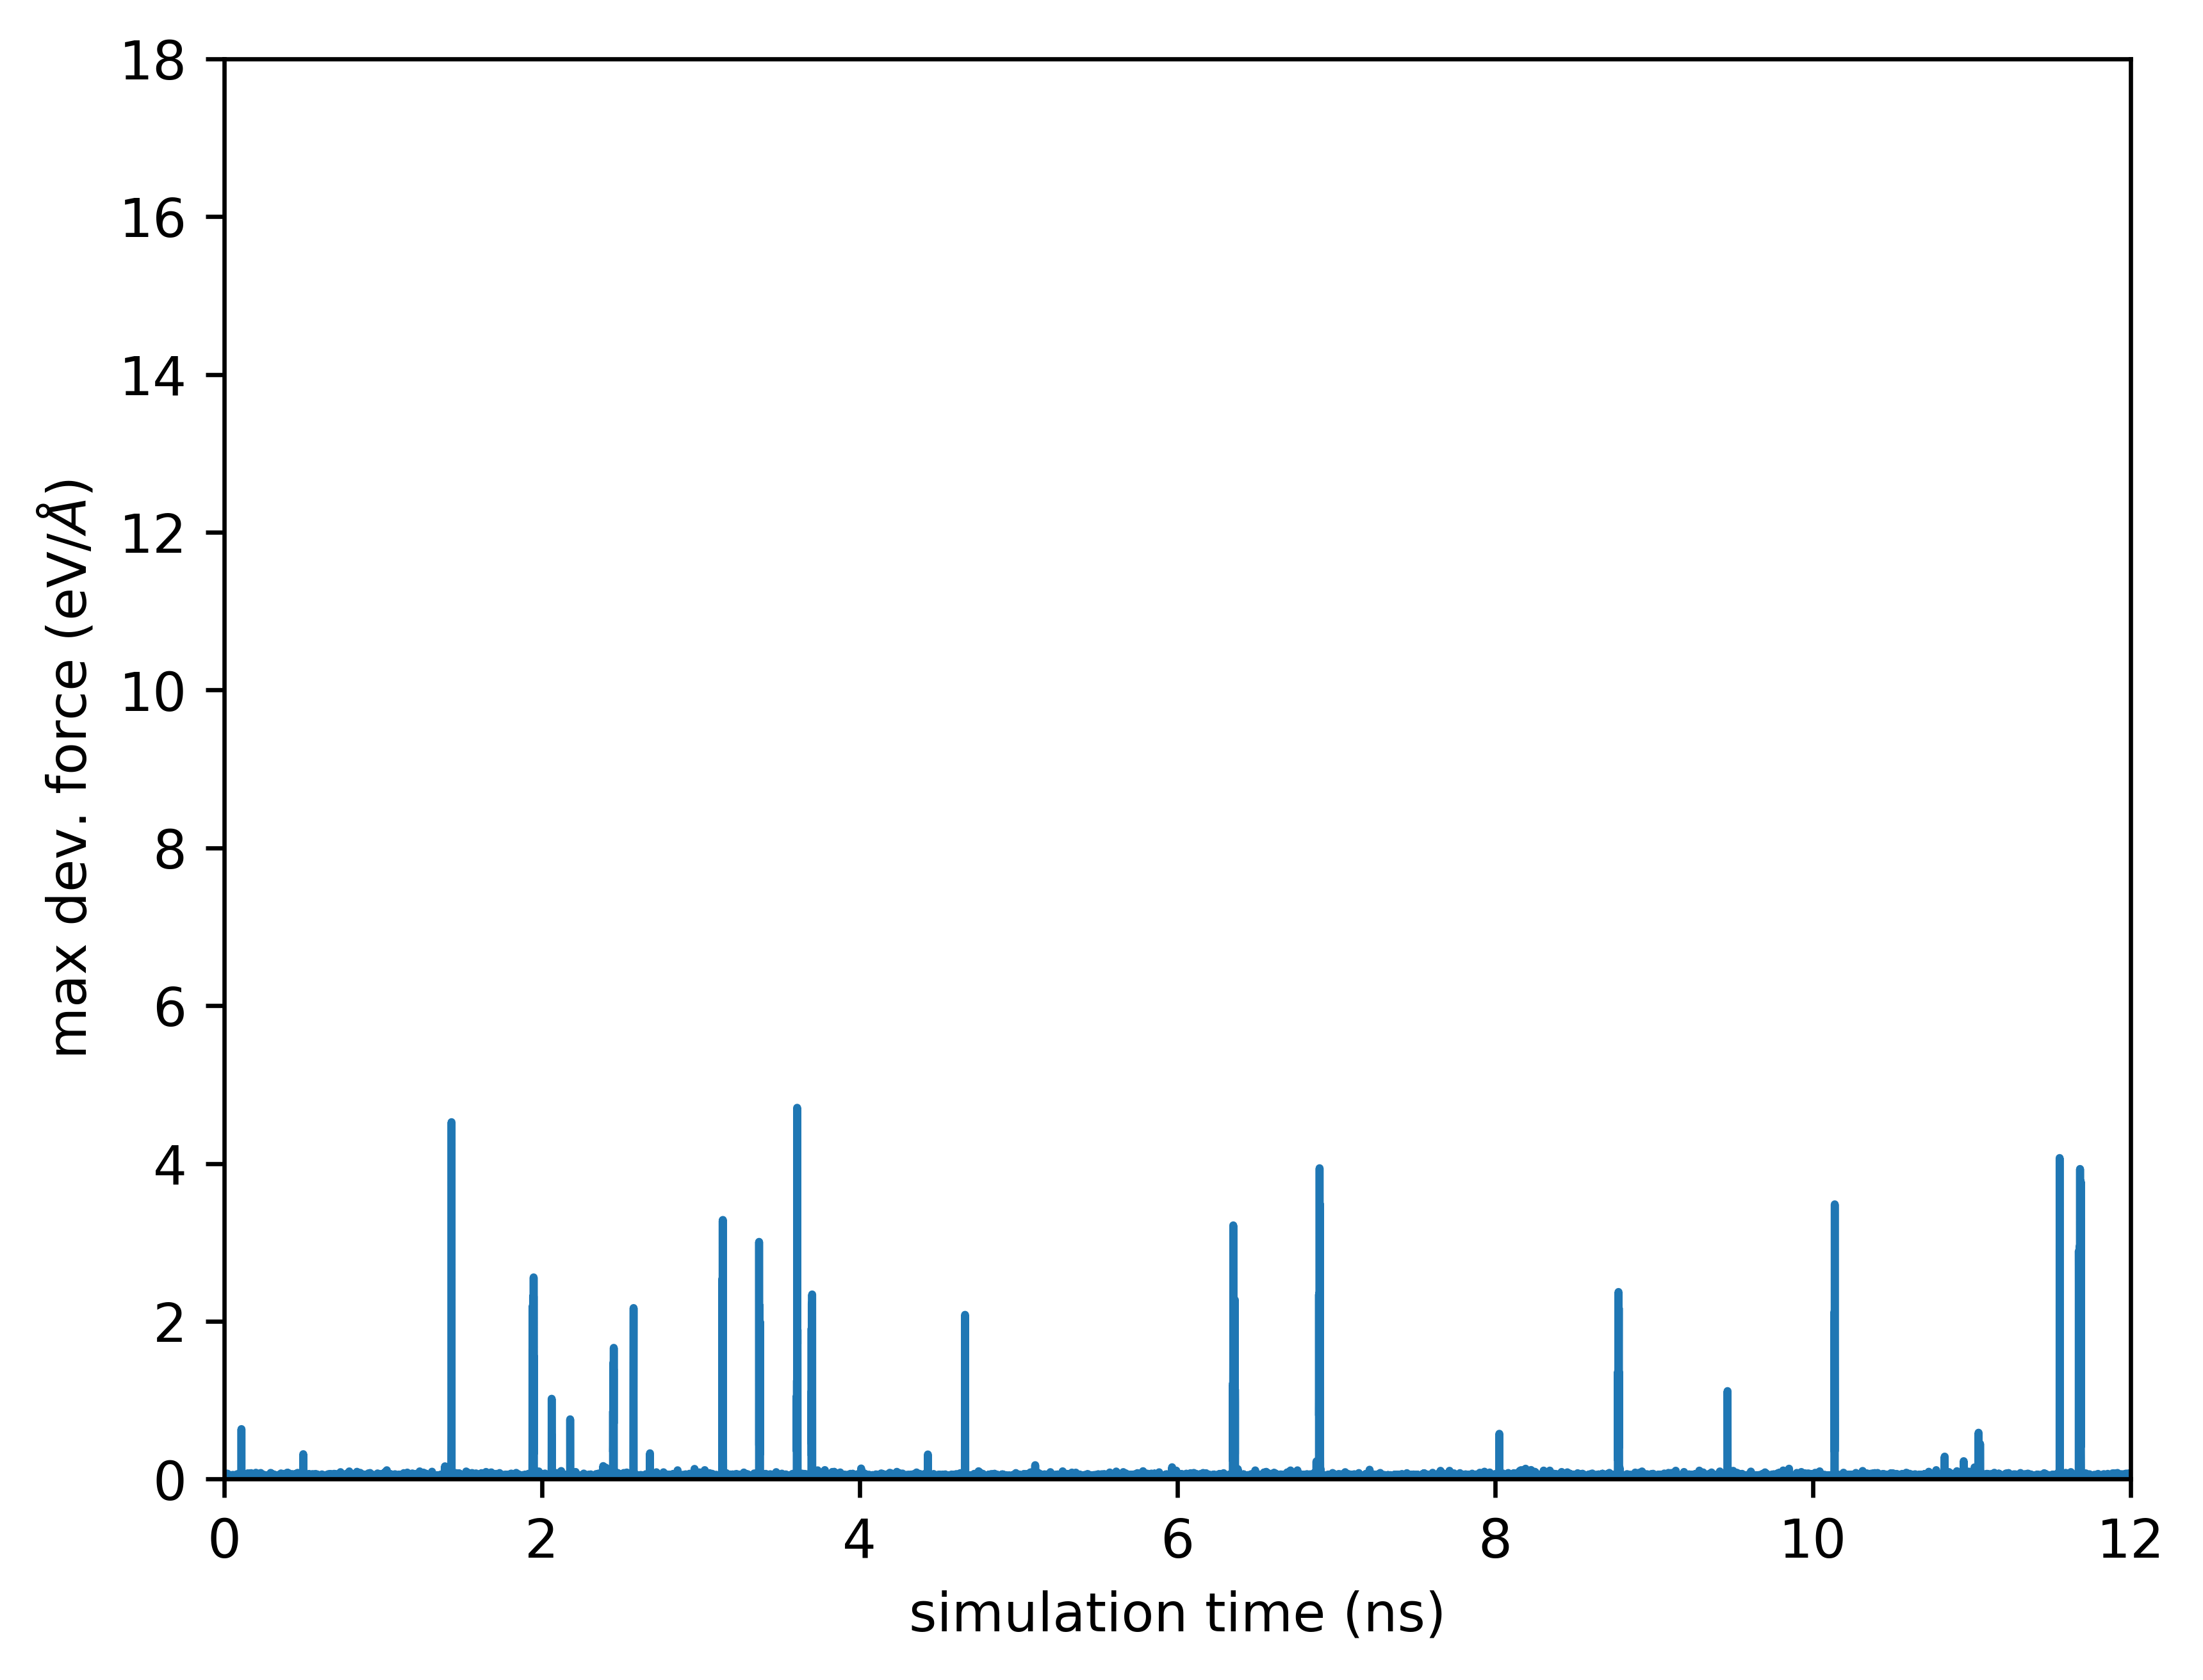
\includegraphics[width=0.9\textwidth]{images/deviation_bulk+interface}
		\caption{Bulk+Interface trained NNP}
		\label{fig:dev_bulk_interface}
	\end{subfigure}

	\caption{Stability of (a) bulk trained NNP and (b) bulk+interface
		trained NNP when used as pair potential in MD simulation of
		interfacial
		systems. }
	\label{fig:model_dev}
\end{figure}

A test was conducted to describe the accuracy of the trained neural network
potentials on prediction of energy, force, and virial with respect to the DFT
data for interfacial systems.
Table~\ref{tab:train_perf} lists the mean absolute
error (MAE) and root mean square error (RMSE) of bulk trained NNP and
bulk+interface trained NNP. It can be observed that the error is lower when the
NNP is trained to include both bulk  and interfaces. This is expected since the
model was trained to explore both the bulk and interface environments.
Specifically, there is 59\% and 14\% improvement in RMSE for energy per number
of atoms and force, respectively, for bulk+interface NNP than bulk NNP.

\begin{table}[tbhp!]
	\centering
	\caption{Performance of bulk trained NNP and
		bulk+interface trained NNP on bulk+interface validation
		dataset.}
	\label{tab:train_perf}
	\resizebox{0.7\columnwidth}{!}{%
		\begin{tabular}{@{}lcc@{}}
			\toprule
			                        & Bulk trained NNP &
			Bulk+Interface trained NNP
			\\
			\midrule
			Energy MAE (eV)         & \num{5.195E-01}  &
			\num{1.939E-01}
			\\
			Energy	 RMSE	(eV)         & \num{6.222E-01}  &
			\num{2.616E-01}
			\\
			Energy MAE/Natoms (eV)  & \num{9.019E-04}  &
			\num{3.366E-04}
			\\
			Energy	 RMSE/Natoms (eV) & \num{1.080E-03}  &
			\num{4.541E-04}
			\\
			Force  MAE	(eV/A)        & \num{4.164E-02}  &
			\num{3.613E-02}
			\\
			Force  RMSE (eV/A)      & \num{5.654E-02}  &
			\num{4.836E-02}
			\\
			Virial MAE (eV)         & \num{5.886E-01}  &
			\num{5.491E-01}
			\\
			Virial	 RMSE (eV)        & \num{7.924E-01}  &
			\num{7.256E-01}
			\\
			Virial MAE/Natoms (eV)  & \num{1.020E-03}  &
			\num{9.533E-04}
			\\
			Virial	 RMSE/Natoms (eV) & \num{1.380E-03}  &
			\num{1.260E-03}
			\\
			\bottomrule
		\end{tabular}%
	}
\end{table}

Alternatively, one can check the correlation between the deep NN prediction
with the DFT data. Figure~\ref{fig:corr_E} shows the total energy points whose
coordinates are
the DFT data
and the predicted ones given
by the neural network, for both bulk trained and bulk+interface trained NNP. In
particular, it can
be seen that the predicted energies for the bulk trained NNP are mostly
underestimated which leads to
higher test error as supported in Table~\ref{tab:train_perf}. On the other
hand,  the forces are in good agreement for both types of NNP models as shown
in Figure~\ref{fig:corr_F}.

\begin{figure}[tbhp!]
	\centering
	\begin{subfigure}{0.47\textwidth}
		\centering

		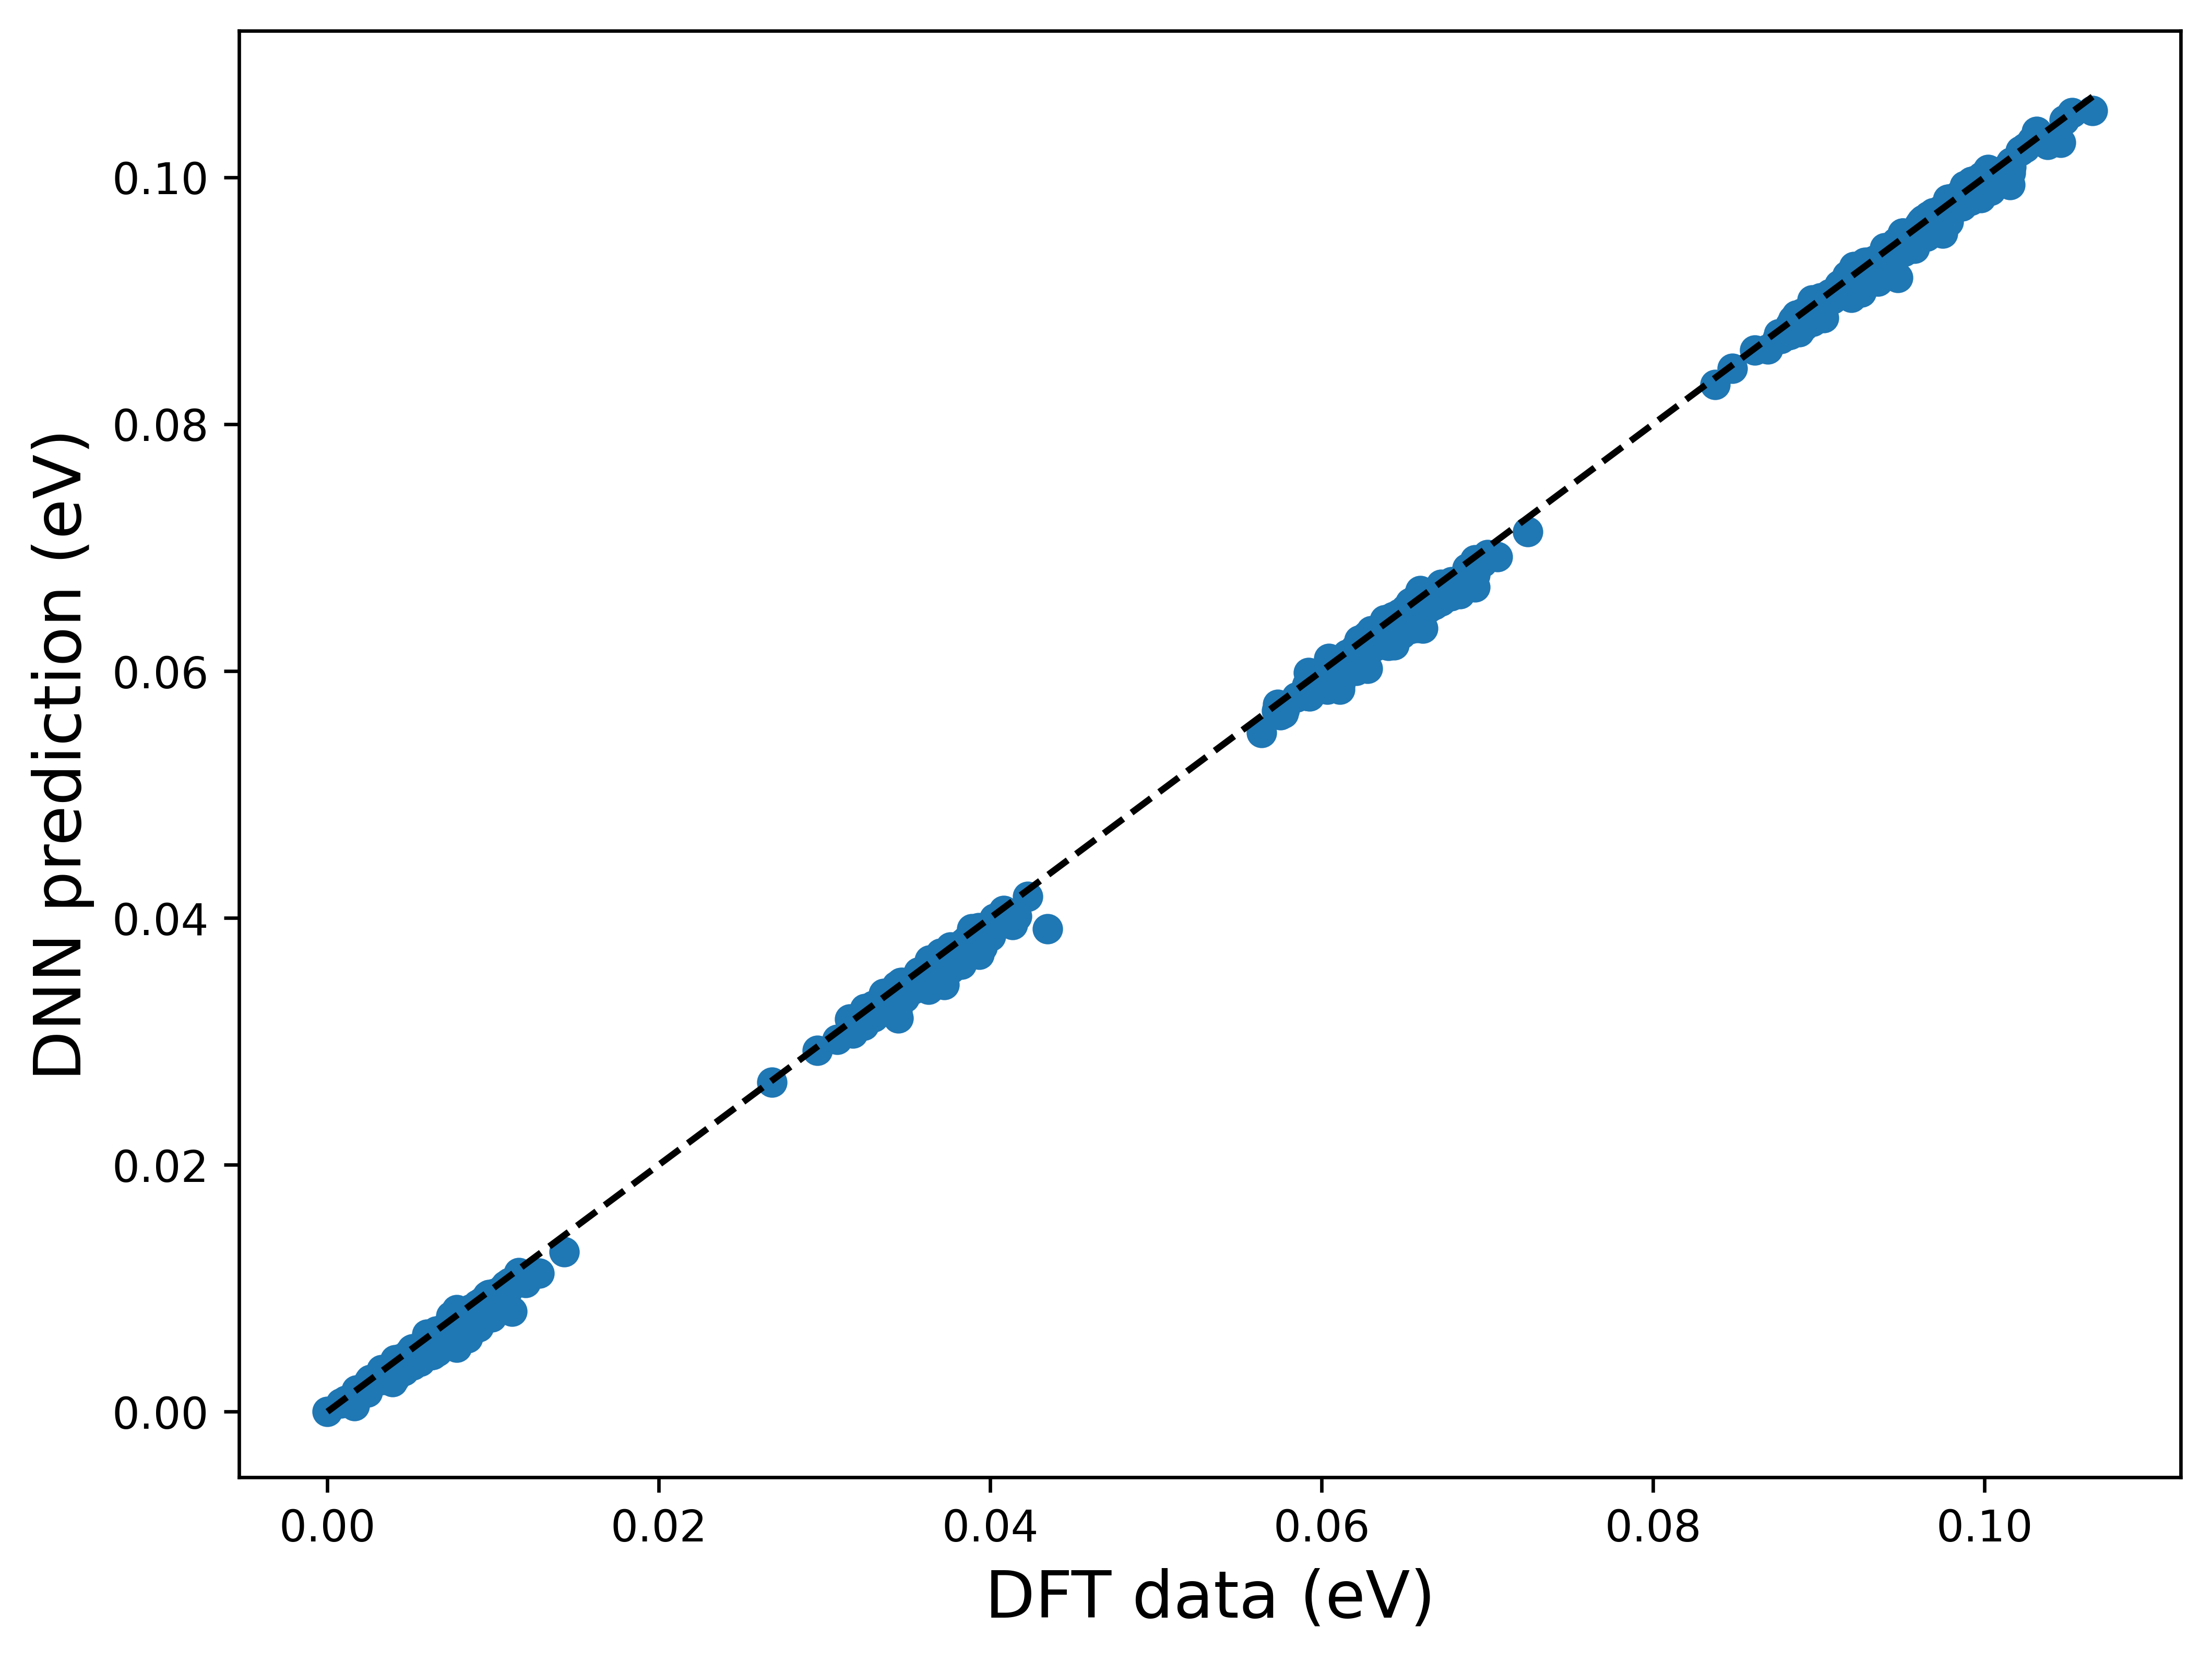
\includegraphics[width=0.9\textwidth]{images/bulk_NN_on_interface/2_e_peratom.png}
		\caption{Bulk trained NNP}
		\label{fig:corr_bulk_NN_E}
	\end{subfigure}
	\hfill
	\begin{subfigure}{0.47\textwidth}
		\centering

		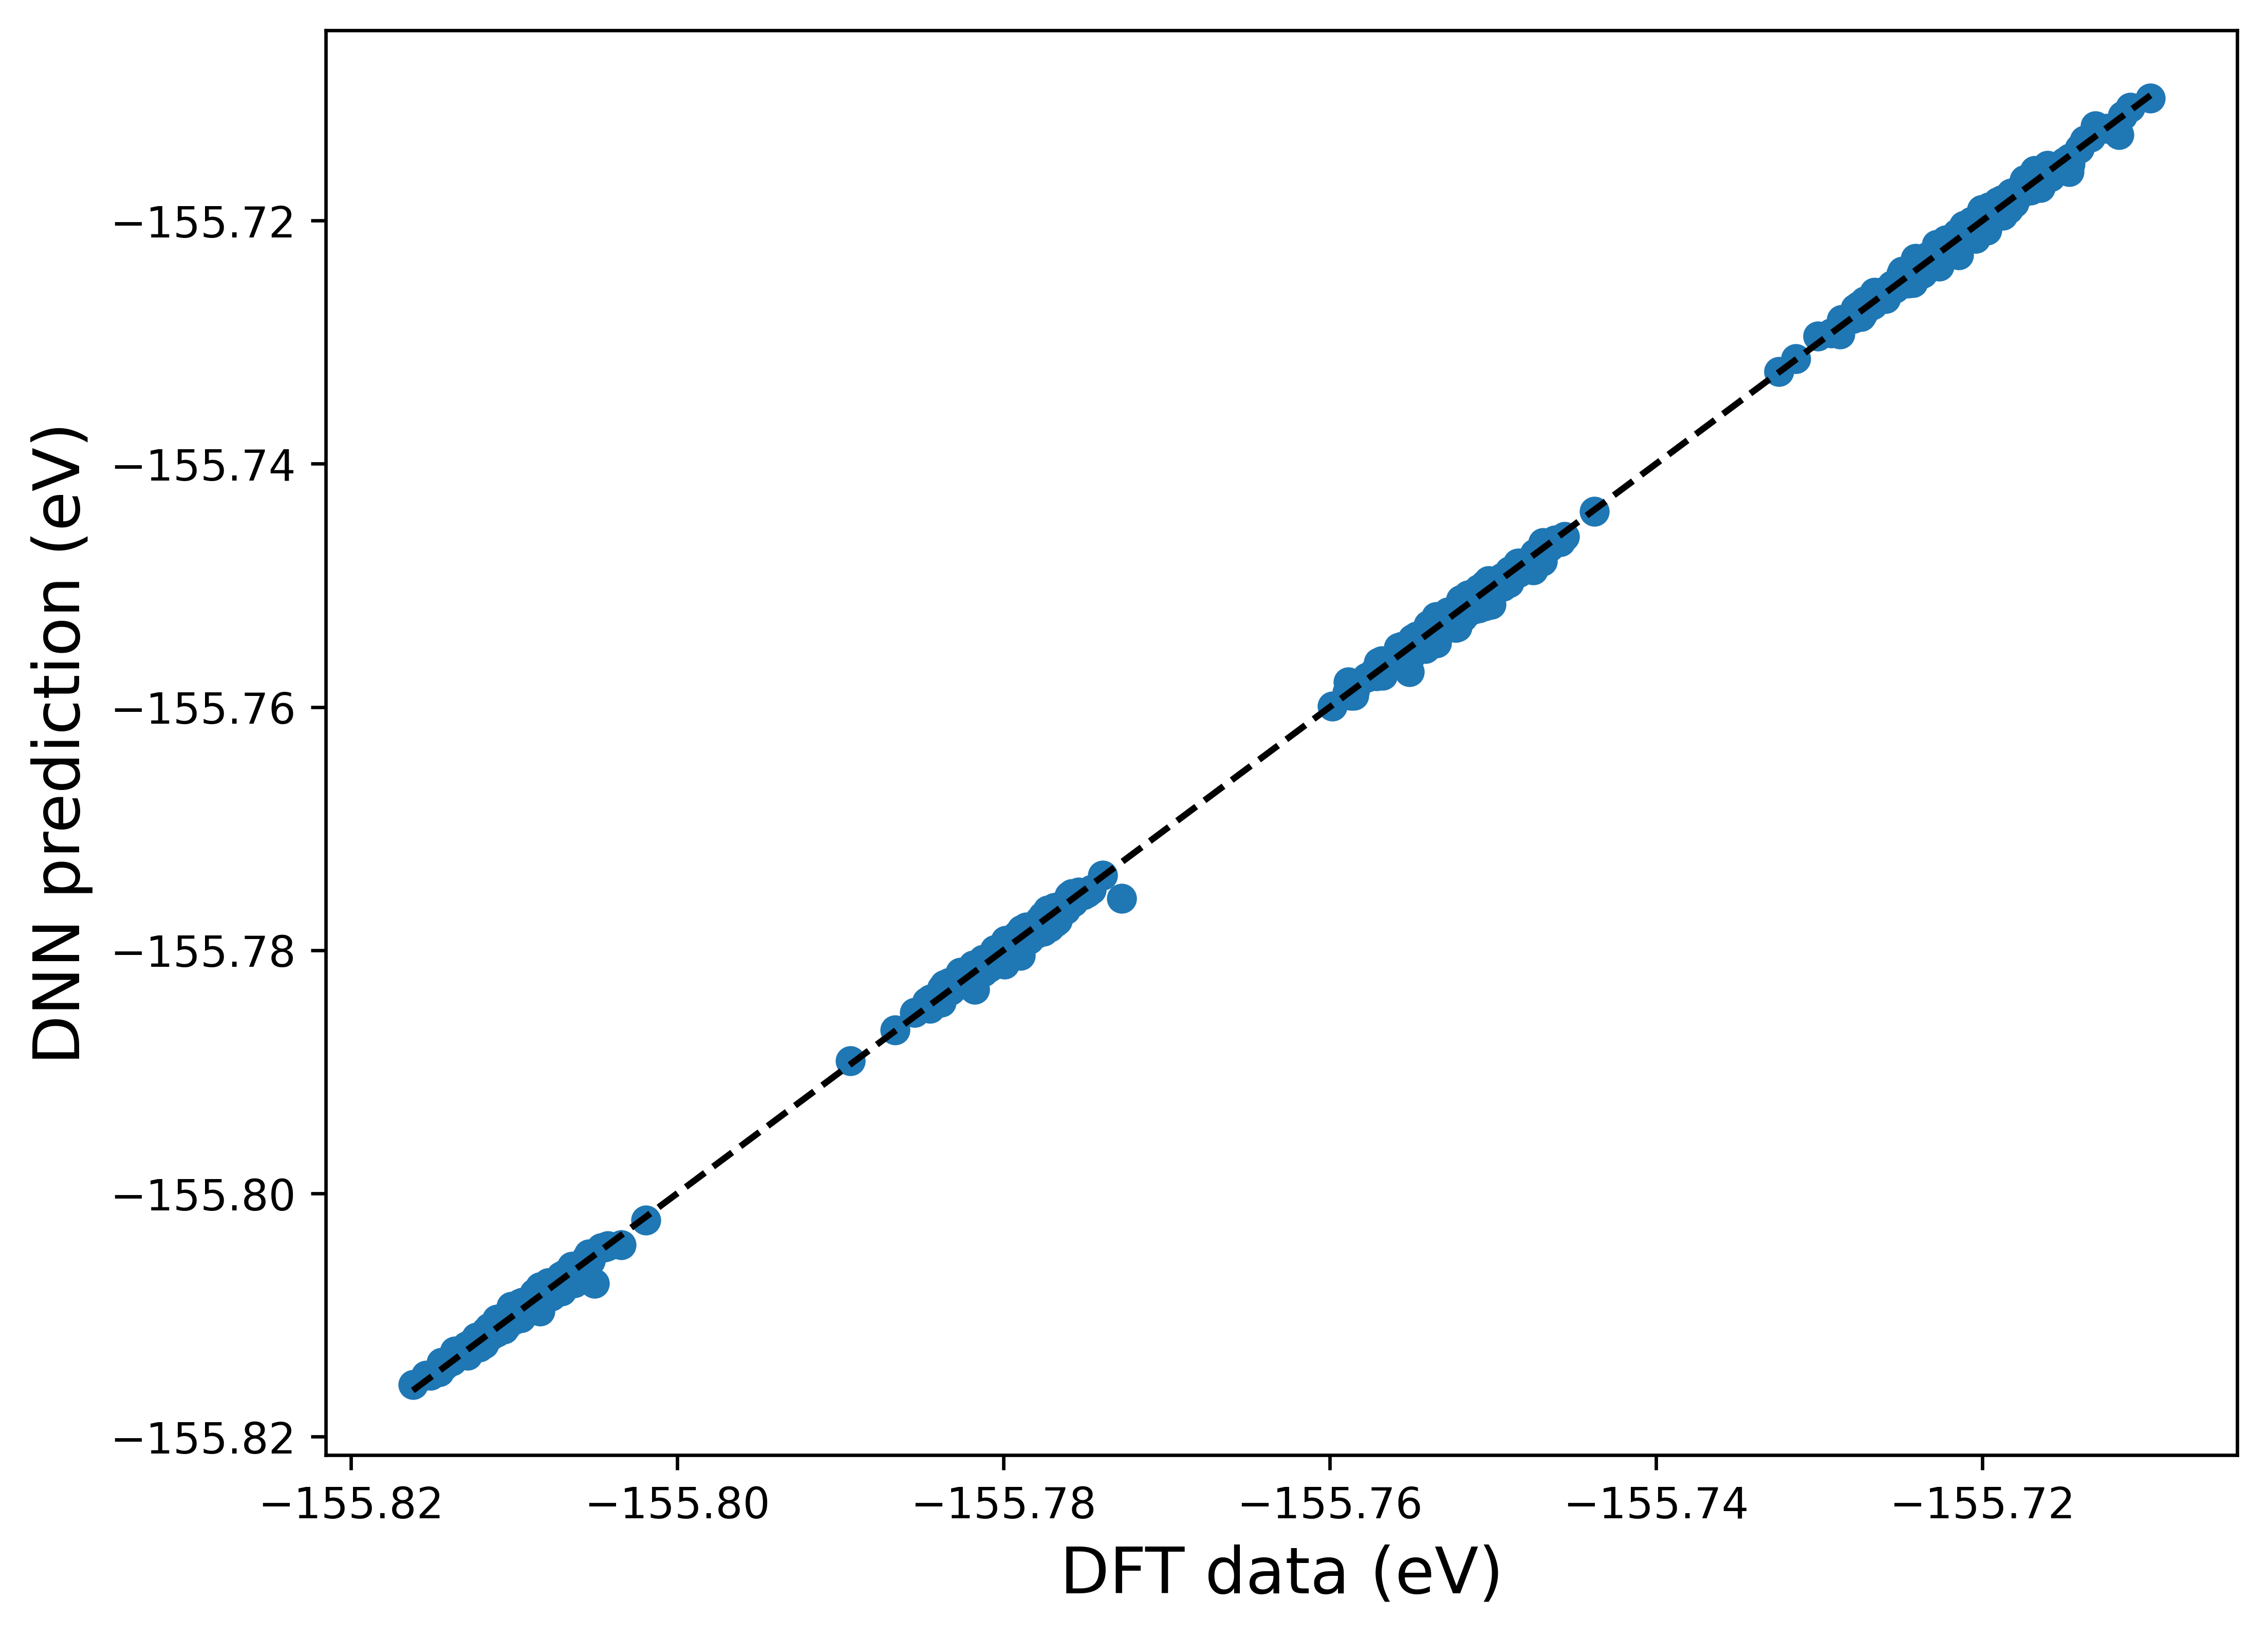
\includegraphics[width=0.9\textwidth]{images/bulk+interface_NN_on_interface/2_e_peratom.png}
		\caption{Bulk+Interface trained NNP}
		\label{fig:corr_bulk+interface_NN_E}
	\end{subfigure}
	\caption{Total energy correlation between deep NN prediction data with
		the DFT data
		for a
		(a) bulk trained NNP model and (b) bulk+interface trained NNP
		model. The
		diagonal line shows the perfect agreement between the two
		data.}
	\label{fig:corr_E}
\end{figure}

\clearpage

\begin{figure}[tbhp!]
	\centering
	\begin{subfigure}{0.47\textwidth}
		\centering

		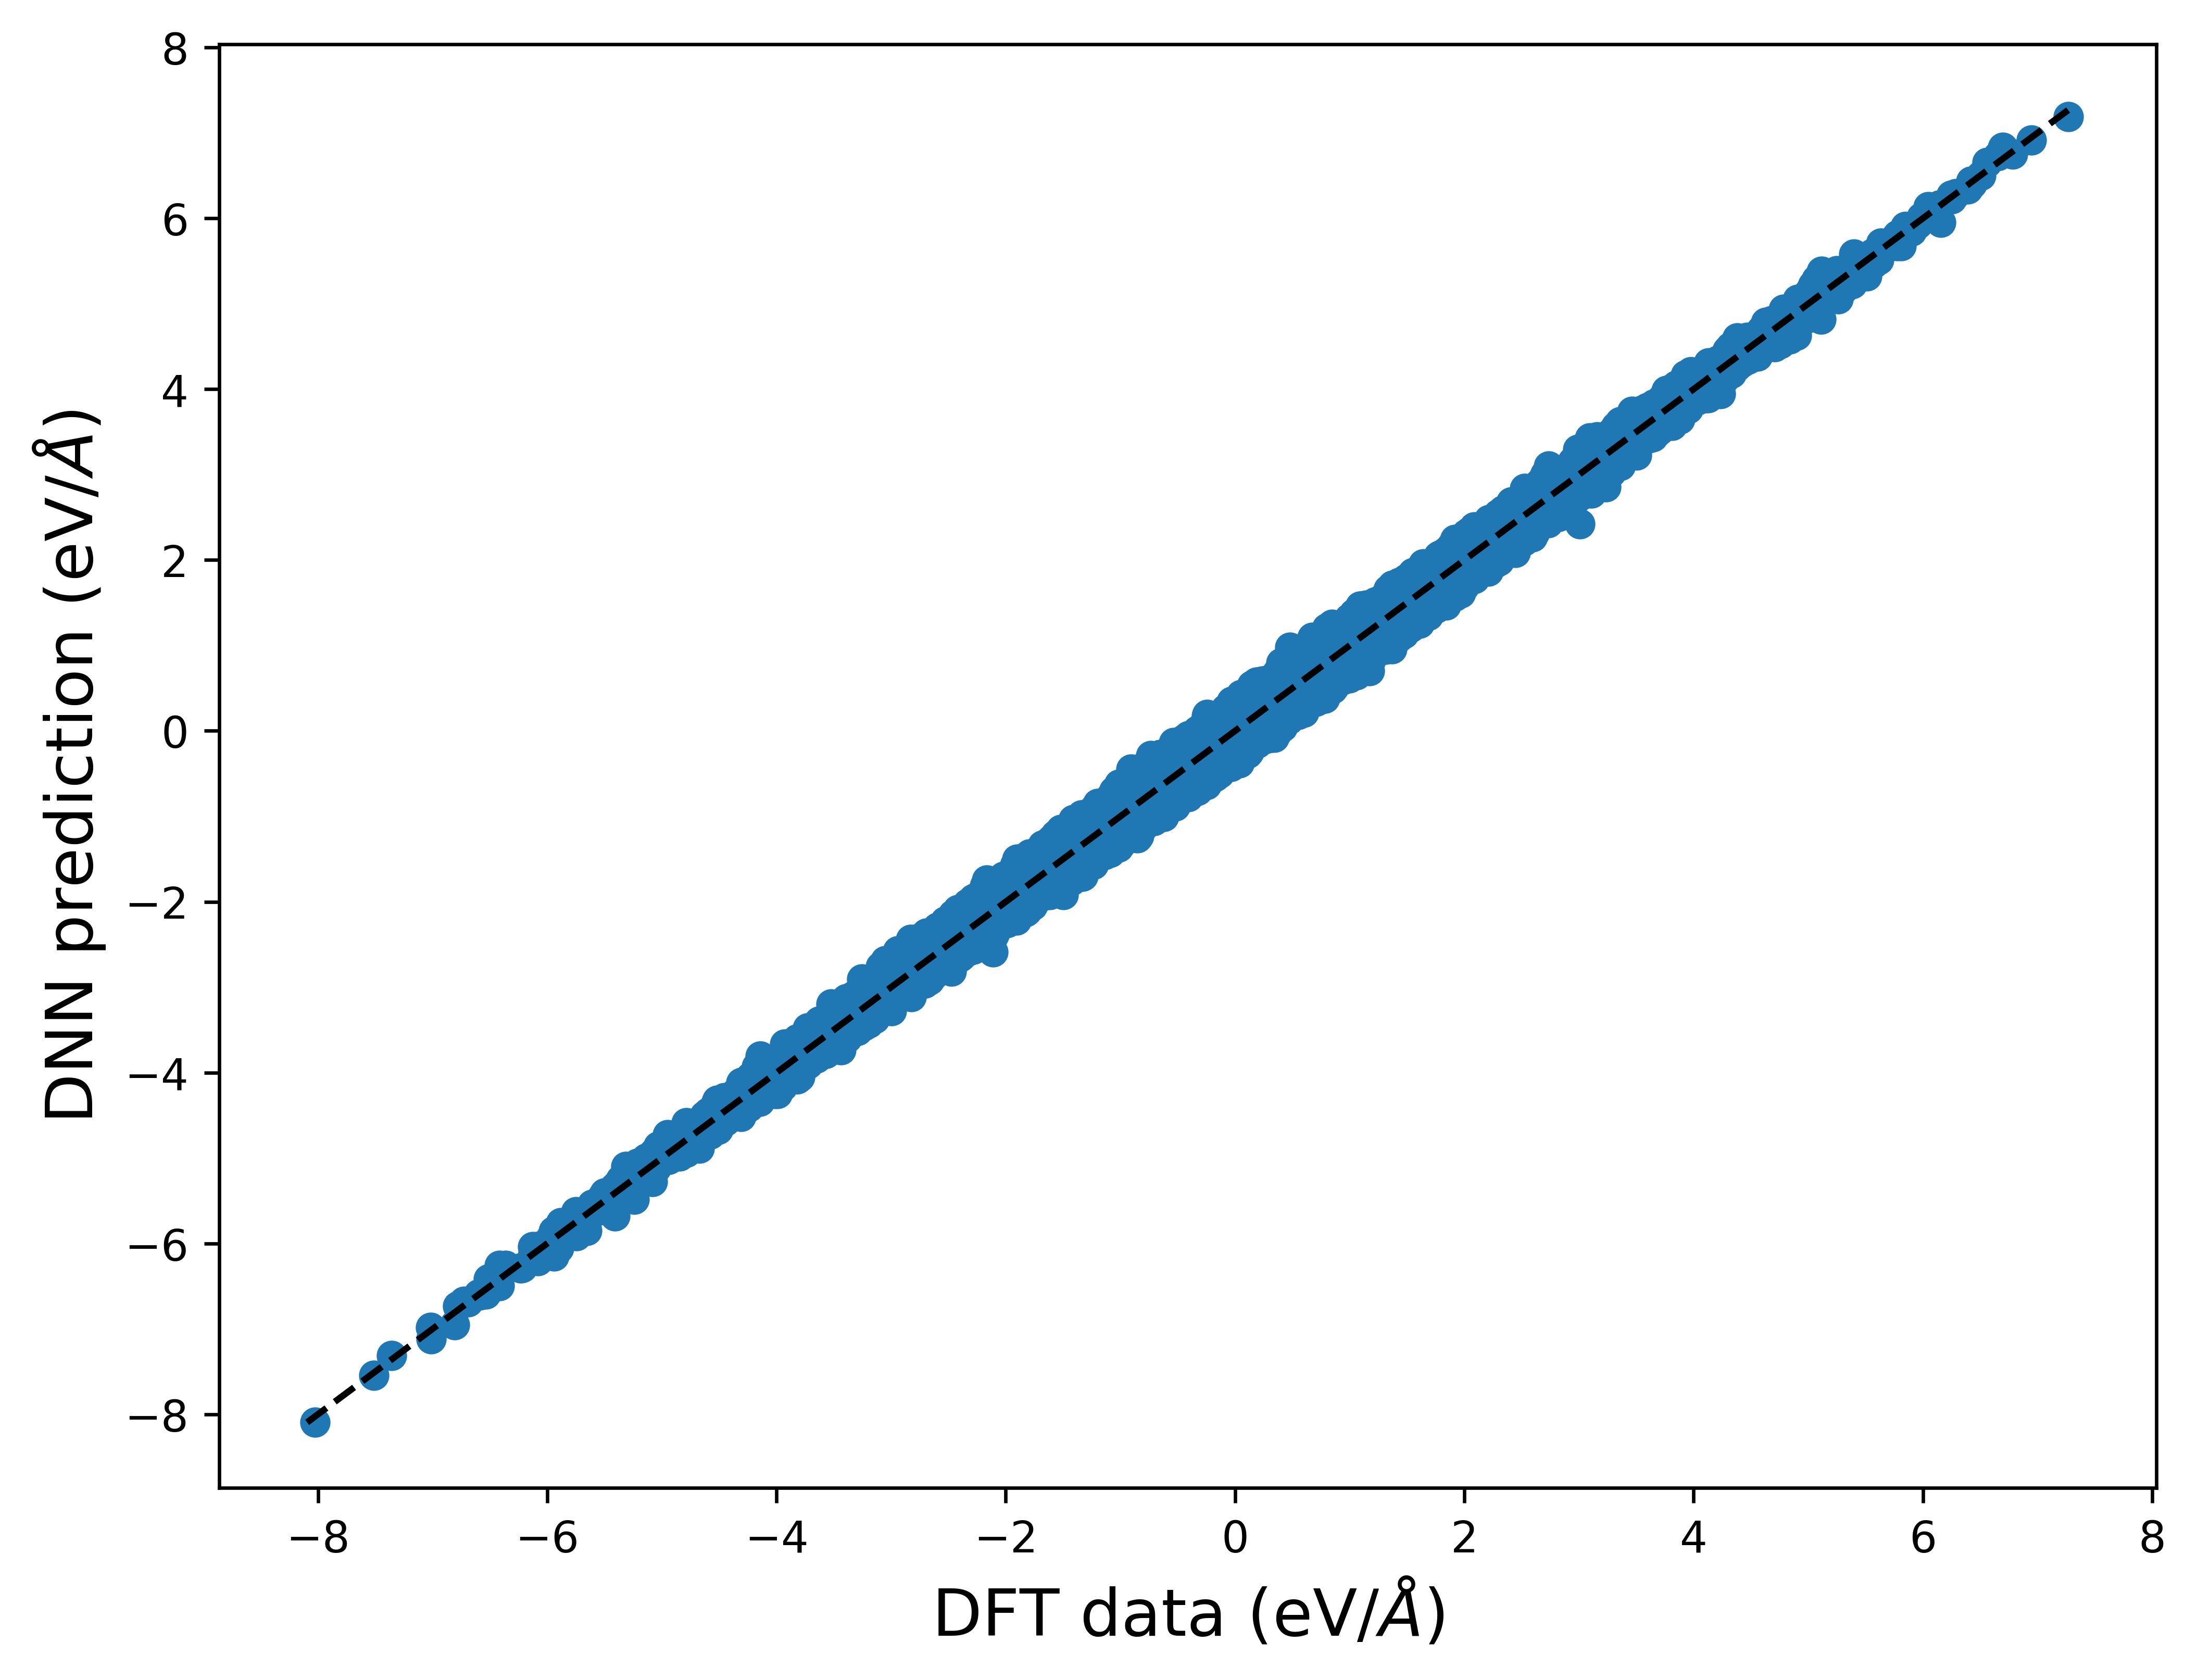
\includegraphics[width=0.9\textwidth]{images/bulk_NN_on_interface/2_force.png}
		\caption{Bulk trained NNP}
		\label{fig:corr_bulk_NN_F}
	\end{subfigure}
	\hfill
	\begin{subfigure}{0.47\textwidth}
		\centering

		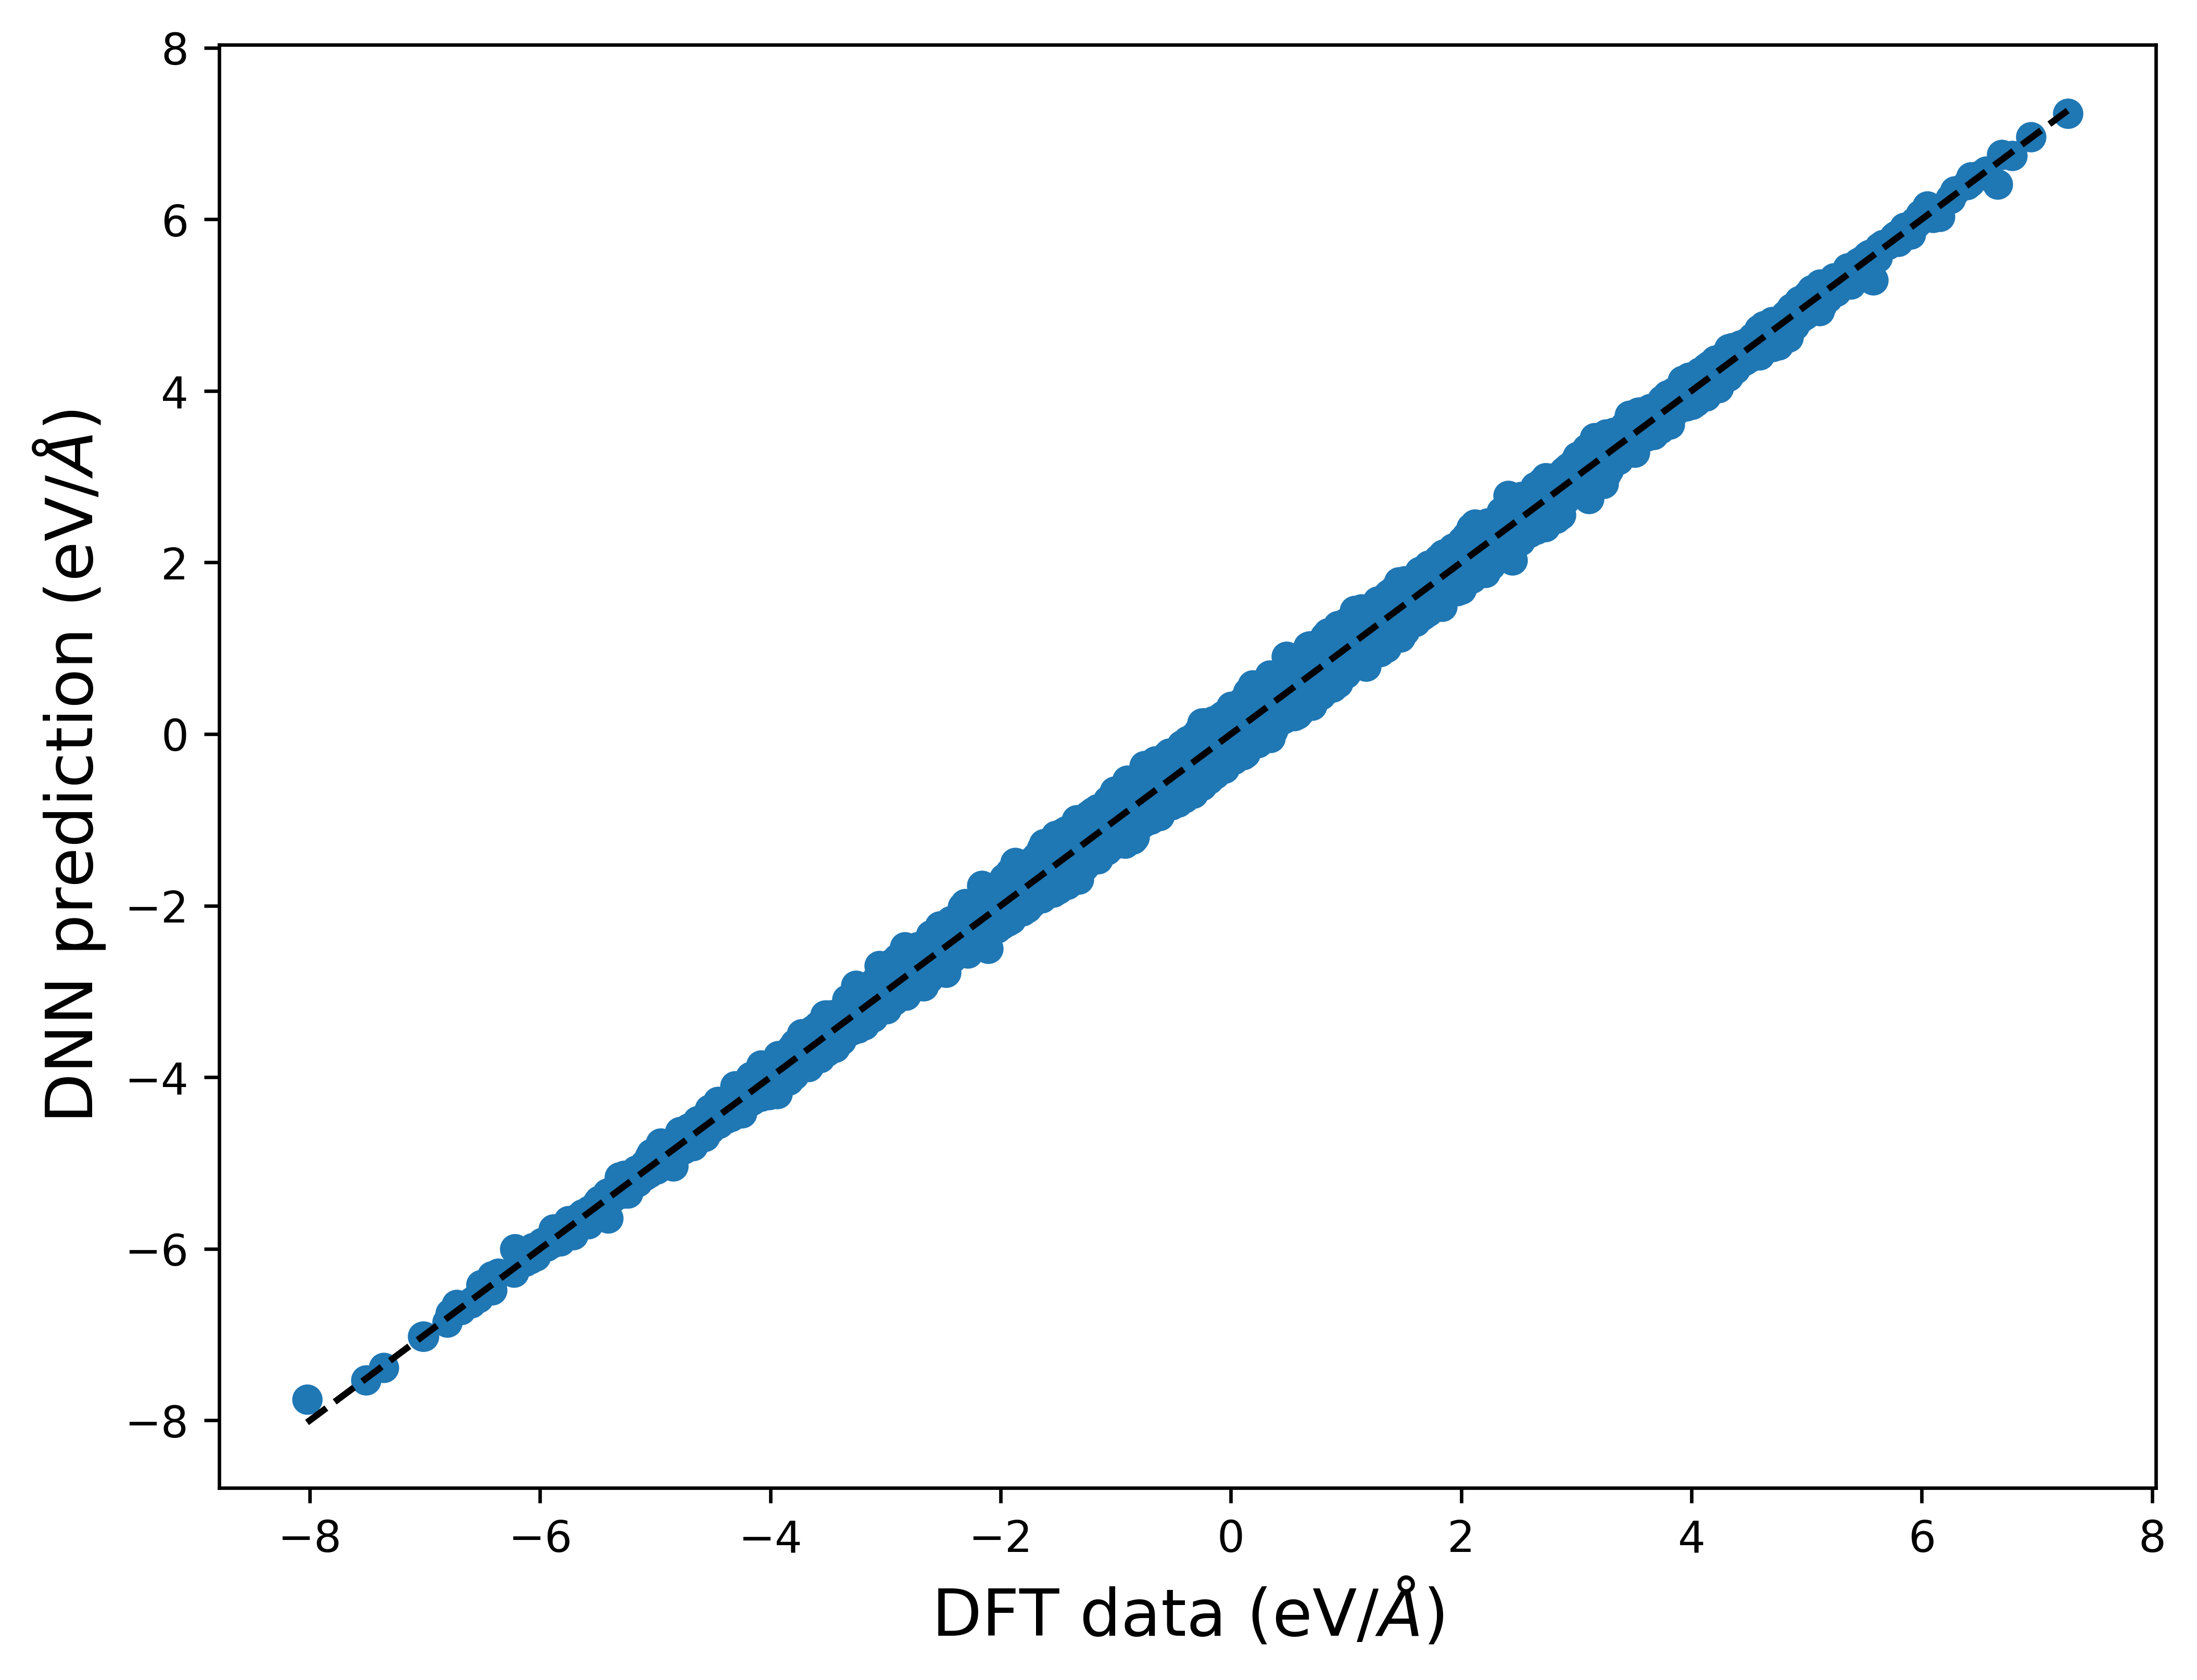
\includegraphics[width=0.9\textwidth]{images/bulk+interface_NN_on_interface/2_force.png}
		\caption{Bulk+Interface trained NNP}
		\label{fig:corr_bulk+interface_NN_F}
	\end{subfigure}
	\caption{Atomic force correlation between deep NN prediction data with
		the DFT data
		for a
		(a) bulk trained NNP model and (b) bulk+interface trained NNP
		model. The
		diagonal line shows the perfect agreement between the two
		data.}
	\label{fig:corr_F}
\end{figure}

\section{Mass Density}
For all MD simulations, the temperature was set at ambient temperature of 300
K. To account the shift of melting temperature of ice when using SCAN
functional,
a shift of +30 K was applied so that 330 K refers to the new ambient
temperature \cite{piaggi2021phase}.

Figure~\ref{fig:density} shows the mass density of 192 water molecules at 330 K
for different deep neural network models. Results of fitting of the mass density profile using Eq.~\ref{eq:fit_dens} are listed in Table~\ref{tab:density_fit}. NNP model trained on bulk
environments has bulk
density of 0.974 \unit{
	g/cm^3} that is underestimated by 2.61\% from the experimental value of 1.00 \unit{
	g/cm^3}. On the other hand, the reference model from the work of
Sanchez-Burgos et
al.~\cite{sanchez2023deep} has bulk density of 1.031 \unit{
	g/cm^3} that is overestimated by 3.09\%. Note that the
reference model was trained on bulk only environments and using SCAN
functional. Meanwhile,
the NNP model trained on  bulk and interface systems has a bulk density of  0.994 \unit{
	g/cm^3} which is the most accurate among the models. In addition, the bulk+interface trained NNP  describes	accurately the bulk region  because the fluctuations of the density values are small in
comparison to the other models. Interfacial thickness was quantified
and the bulk+interface trained NNP has the smallest thickness of 1.360 \unit{\angstrom} among the models followed by reference NNP of thickness 1.410  \unit{\angstrom} then the bulk trained NNP of thickness 1.546  \unit{\angstrom}. Experimental measures of the interfacial thickness are of the order of 3.2 \unit{\angstrom} \cite{braslau1985surface}, about twice larger than the obtained values from NNP models. The large discrepancy has been
attributed to the suppression of capillary waves due to the finite size of  the simulation cell \cite{matsumoto1988study}.




\begin{figure}[tbhp!]
	\centering
	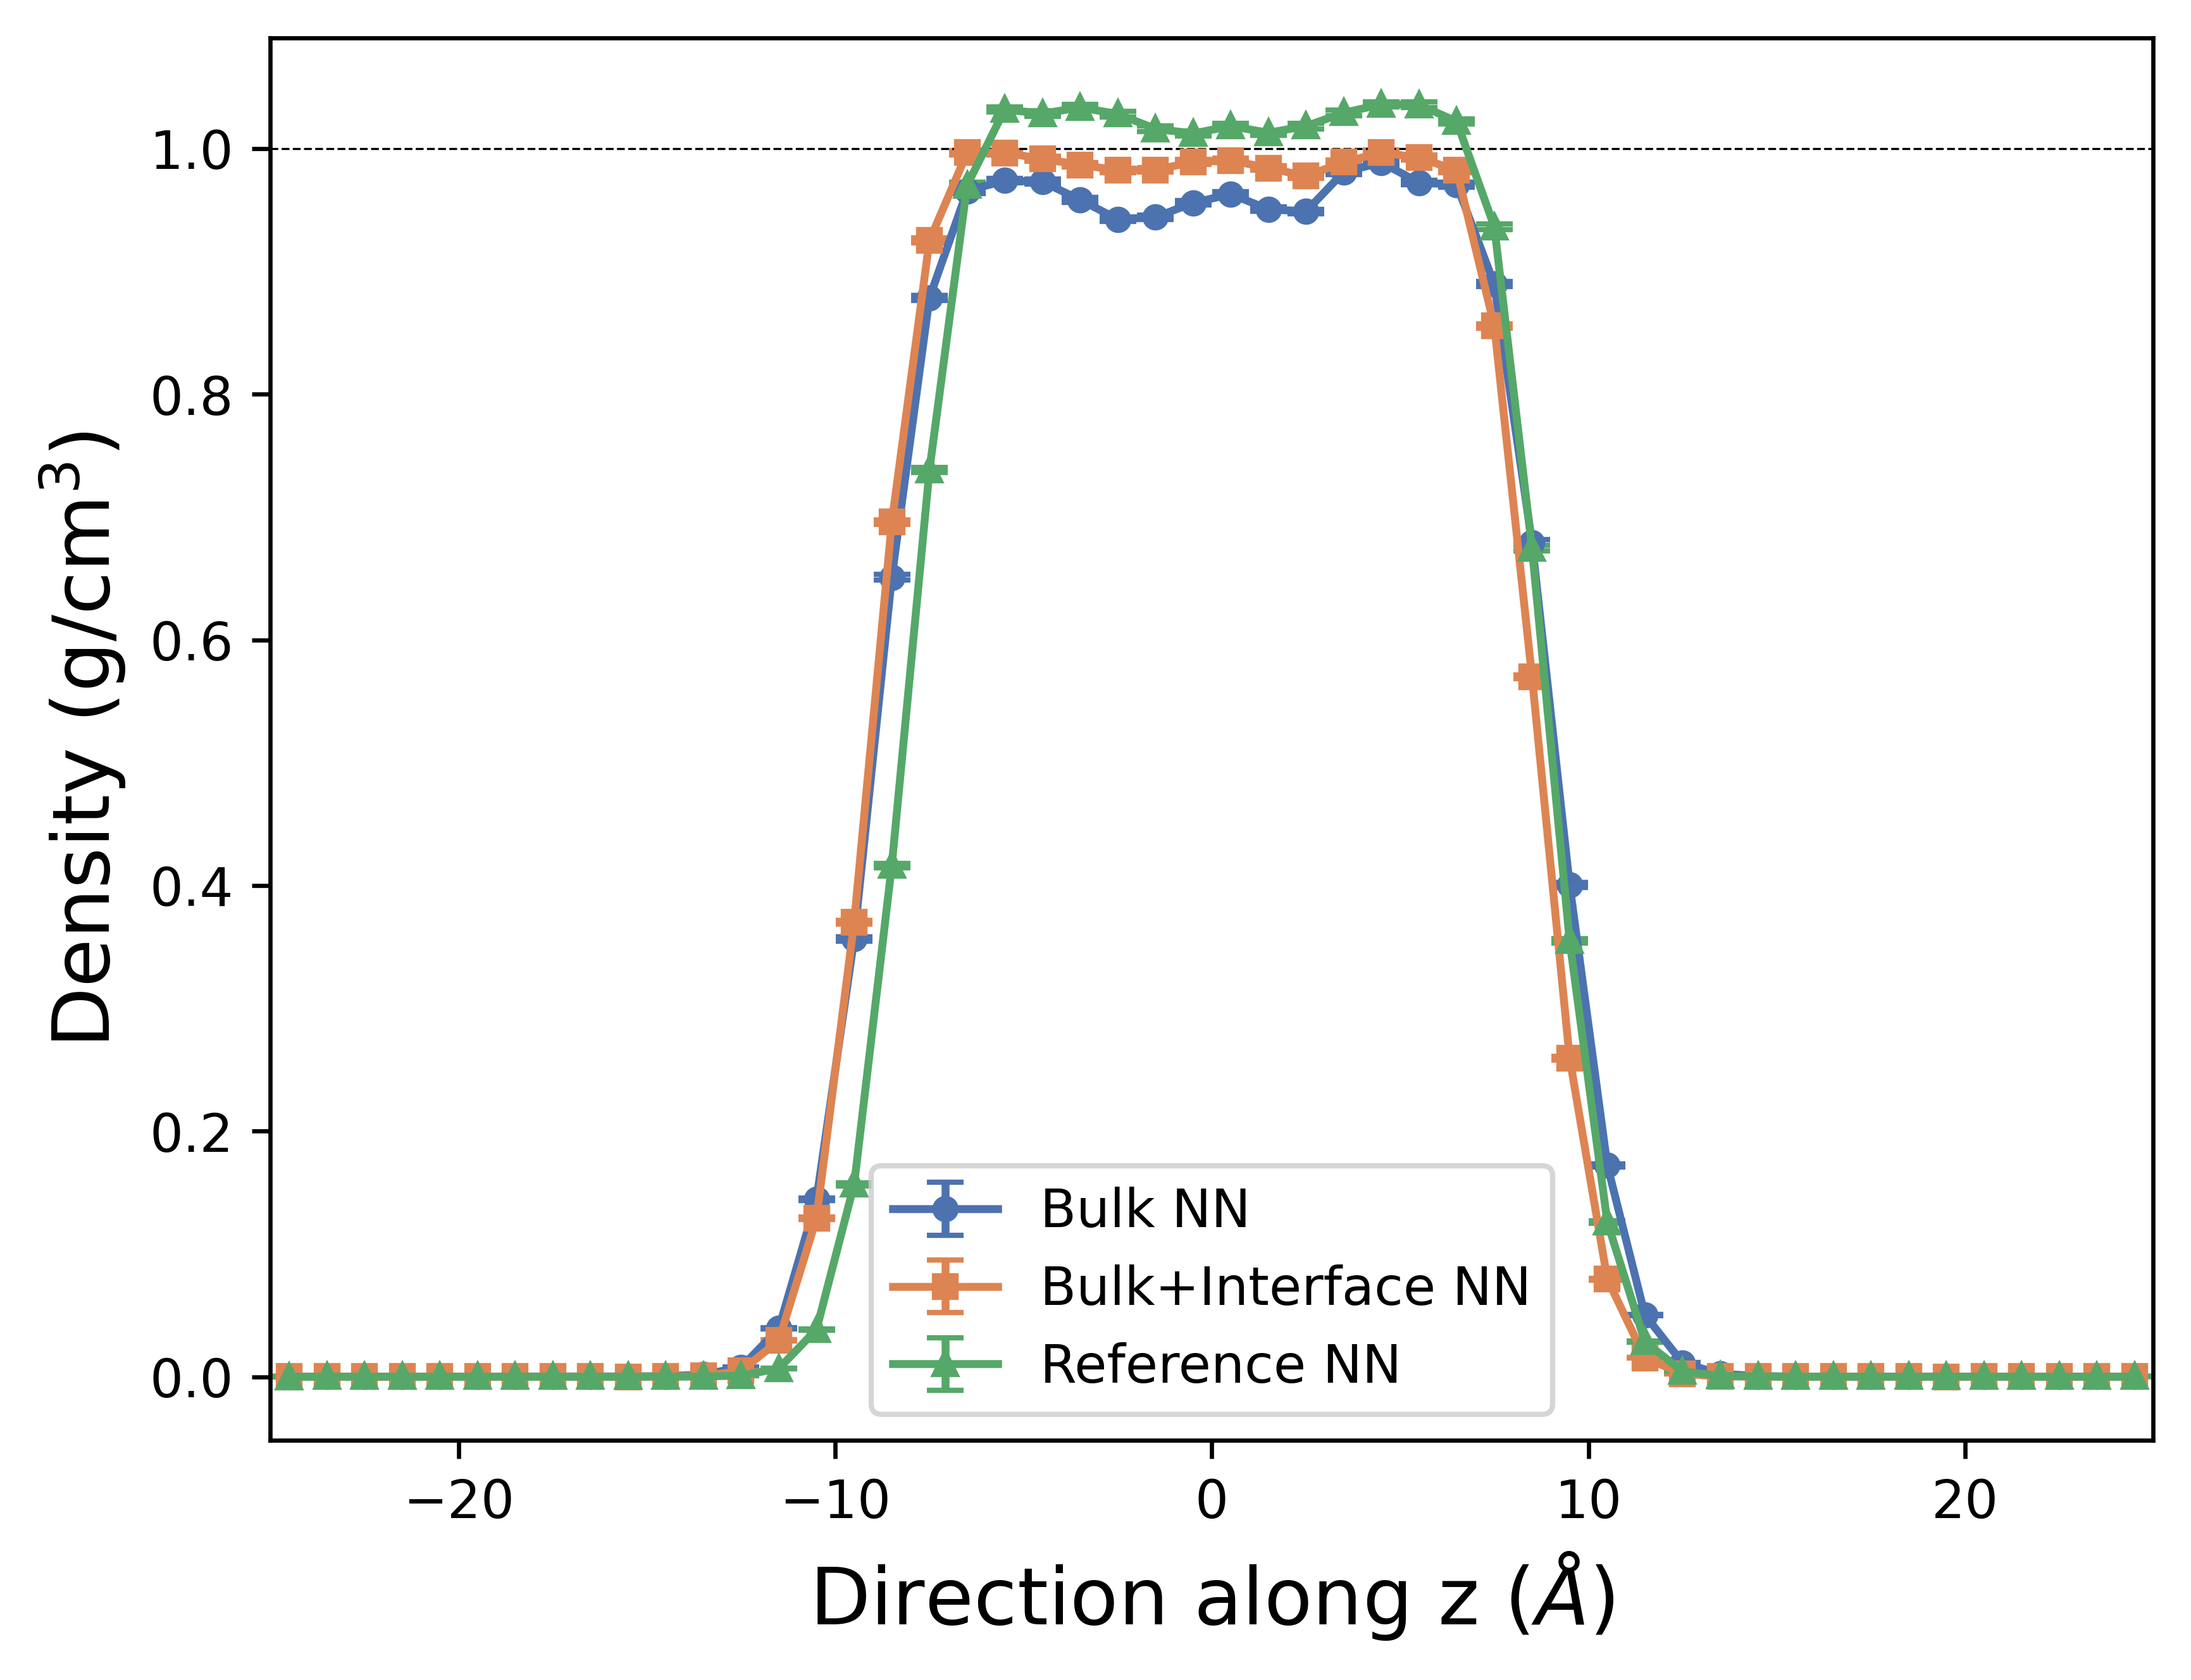
\includegraphics[width=0.65\linewidth]{images/density_330.png}
	\caption{Mass Density Profile at 330 K for different deep neural
		network
		models. The reference model is based on trained model of
		Sanchez-Burgos et
		al.~\cite{sanchez2023deep}. }
	\label{fig:density}
\end{figure}


\section{Surface Tension}
Surface tension was calculated according to formula in Eq.
\eqref{eq:surf_tens}. It is expected that for a bulk system, this equation will
give zero since there is isotropy of pressure in all directions. However, for
systems with interfaces, there will be a broken symmetry along the direction
normal to the surface, which will effectively get nonzero surface tension.

Figure~\ref{fig:surf_tens} shows the plot of the surface
tension as a function of temperature for different NNP models. The bulk-only
trained NNP model has very poor results that is greatly underestimated and
starts to plateaus at above 400 K. Meanwhile, the bulk+interface trained NNP
model
improved the surface
tension much better than  bulk-only trained NNP model, and gets much better at
higher
temperature. This result supports the idea that surface defects play a role in
predicting
the interfacial properties such as surface tension. The reference
model is more accurate even though the model was trained on  bulk only
environments. However, the reference model was trained for a very large
training dataset that includes both ice and liquid phases and vast
thermodynamic range up to 2000 K and 50 GPa \cite{zhang2021phase}. However, our
bulk+interface trained NNP model was trained on thermodynamic range up to 600 K
and 1 GPa, and still give comparable accuracy as the reference model.

\begin{figure}[h!]
	\centering
	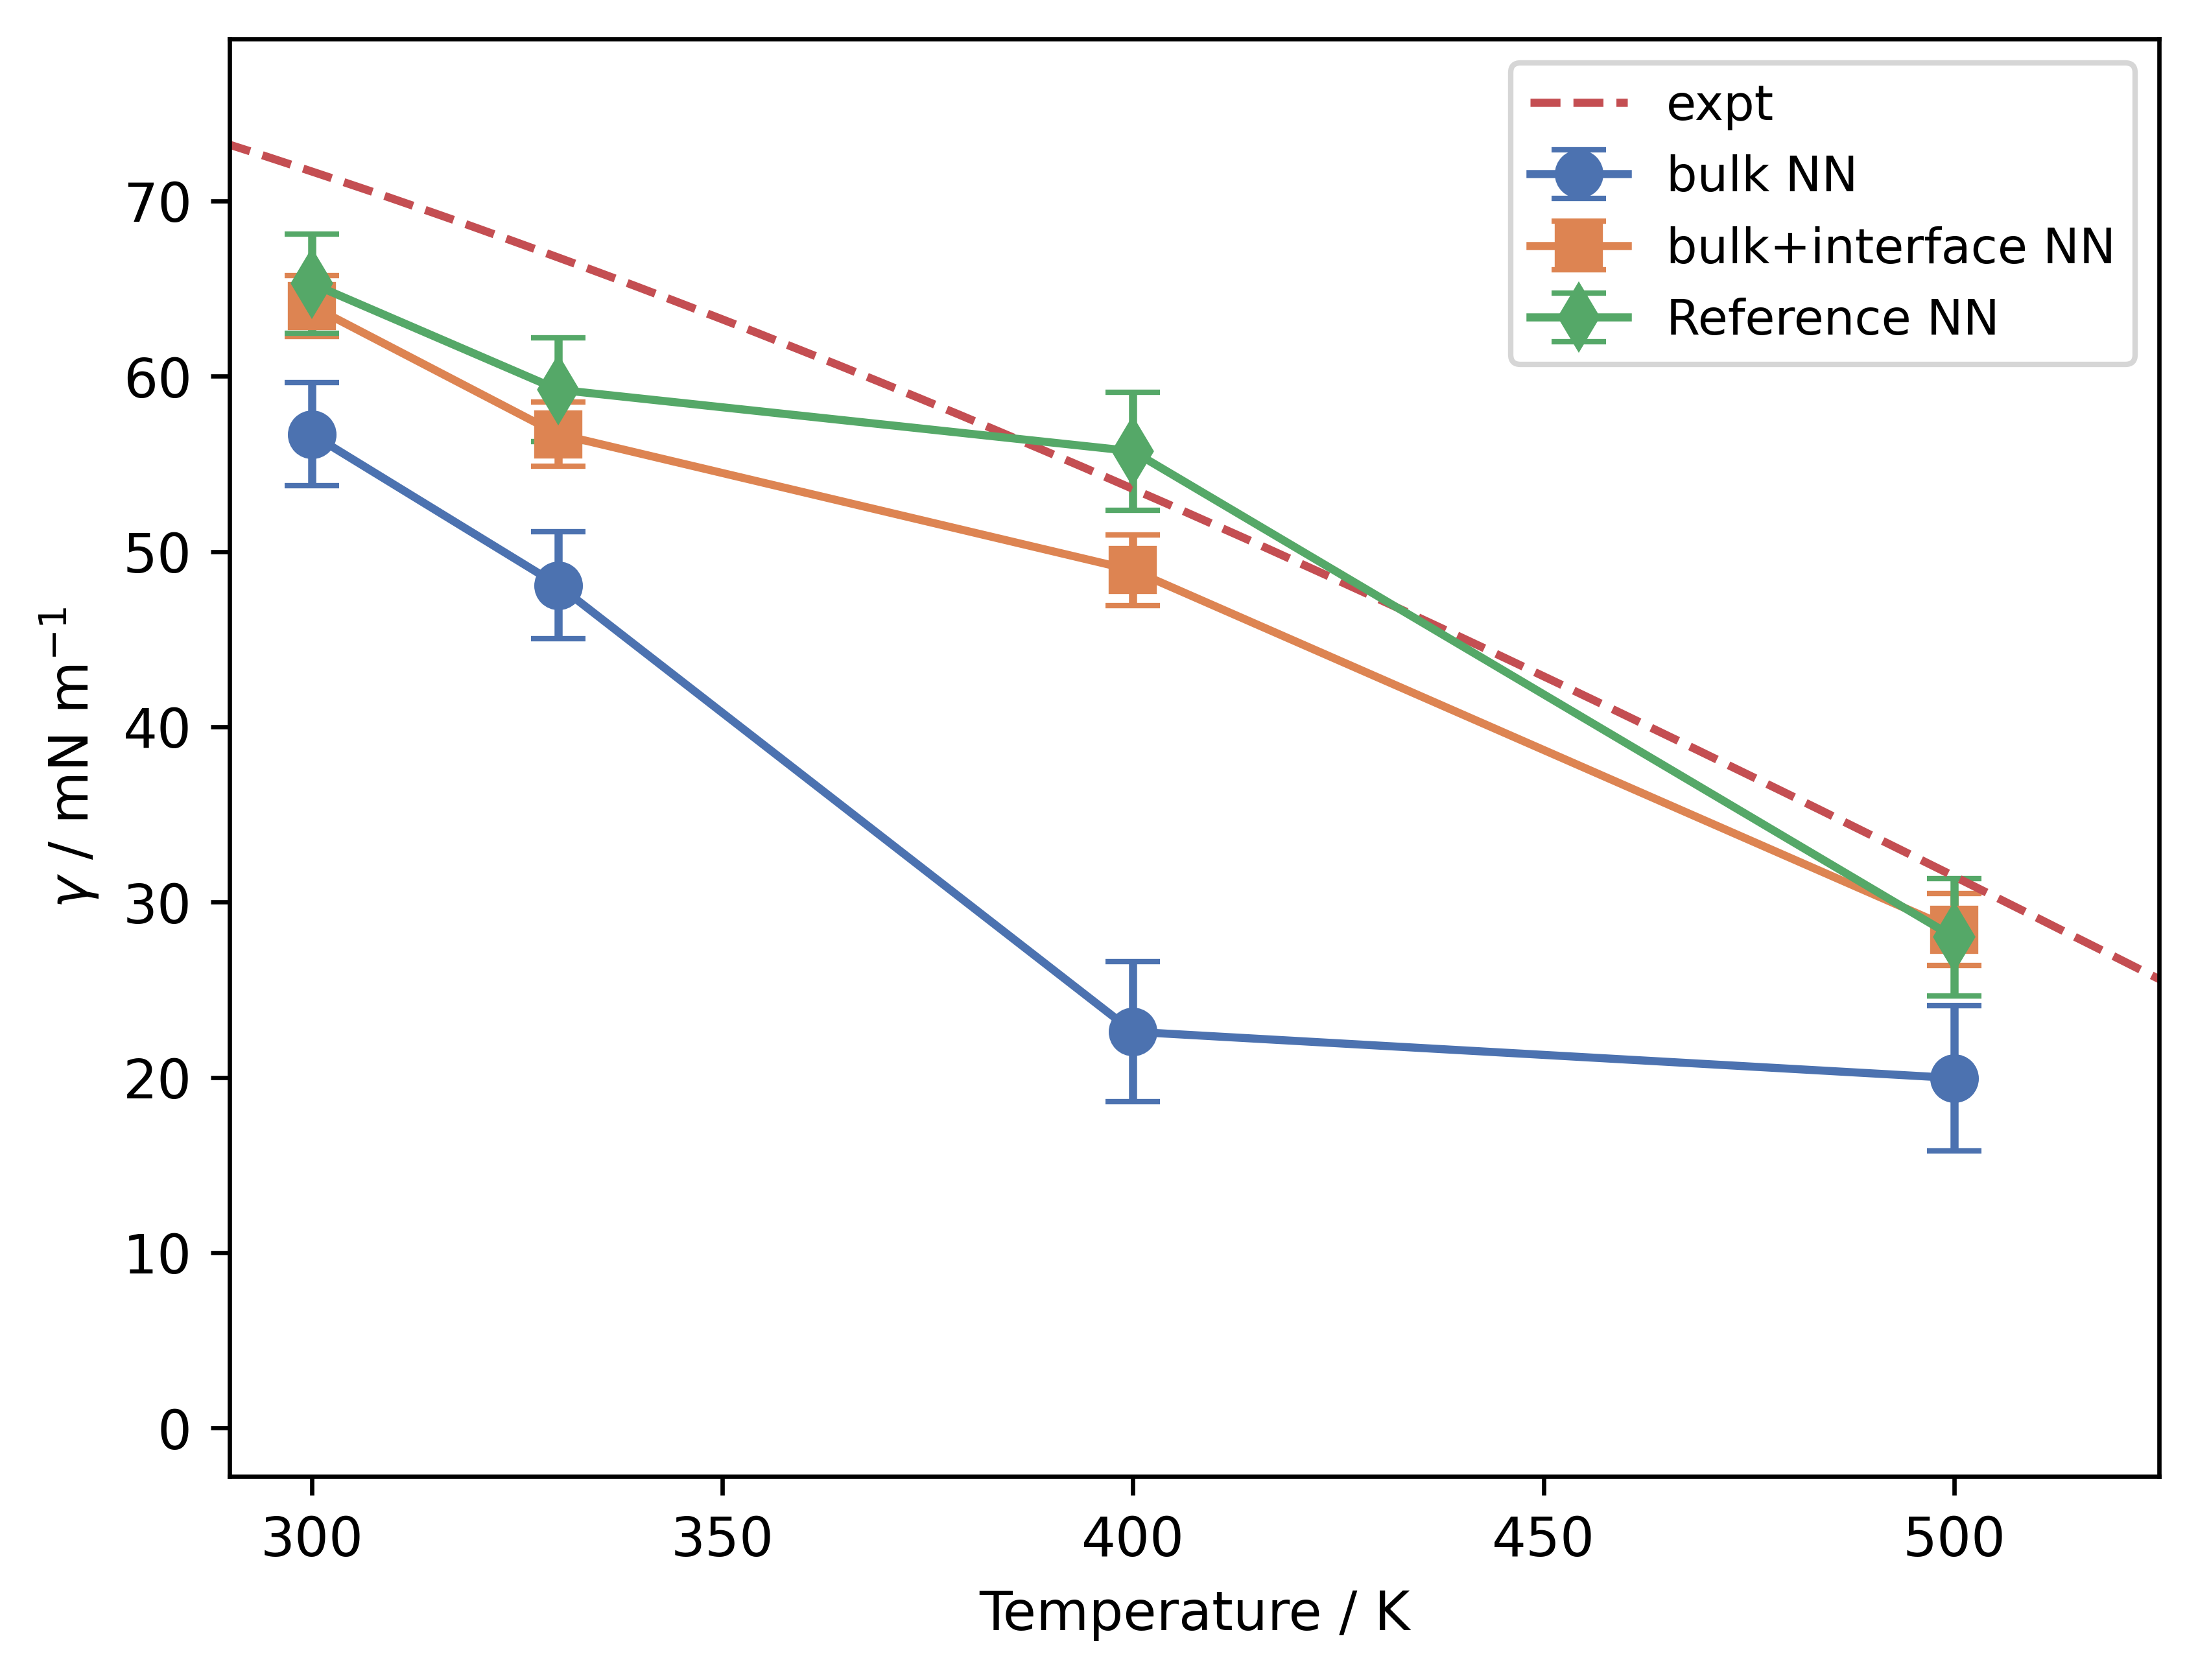
\includegraphics[width=0.7\linewidth]{images/surface_tension.png}
	\caption{Surface tension for different NNP models. The
		reference model is based on trained model of Sanchez-Burgos et
		al.~\cite{sanchez2023deep}.  }
	\label{fig:surf_tens}
\end{figure}

\section{Dipole Orientation}
One way to get microscopic properties of the system is by calculating the
distribution of
average dipole moment orientation. Specifically, the $\cos(\theta)$ was
computed where
$\theta$ is
the angle between the dipole moment and the outward normal vector of the
surface as
schematically shown in Figure~\ref{fig:dipole_scheme}. Positive values
correspond to alignment of the dipole with the outward normal
vector. Experimental techniques such as vibrational sum frequency spectroscopy
have shown that
the imaginary component of nonlinear susceptibility changes sign twice
\cite{fan2009structure},
implying  preferential orientation of water at the
interface that forms two layers. As shown schematically in Figure~\ref{fig:dipole_expt}, the water molecule in the first layer will align such that one of the OH bond points to the vapor
phase. The net dipole dipole moment from these covalent bond will orient slightly
towards the surface. Moreover, between the first and second layer, there are
hydrogen bonds that can produce an effective dipole moment that have opposite
direction as the former. These are shown as arrows in Figure~\ref{fig:dipole_guide}. Therefore, it is expected to have a flip in dipole orientation distribution at the interface.

However, only one type of orientation is observed for the  different NNP models, as shown in Figure~\ref{fig:dipole_orient}. The NNP model trained with bulk and surface environments have an
opposite dipole
orientation compared to models that were trained on bulk only. It can be hypothesized that the bulk+interface trained NNP enhances the dipoles that are pointing down meanwhile the bulk trained NNP enhances dipole that are pointing up.

In addition, it can be
observed that the bulk region has non zero dipole moment which may be caused by
small system size which enhances finite size effects. It is expected that there is zero net
dipole moment inside the bulk due to random thermal reorientation of water
molecules and by symmetry.

\begin{figure}[tbhp!]
	\centering
	\begin{subfigure}{0.47\textwidth}
		\centering

		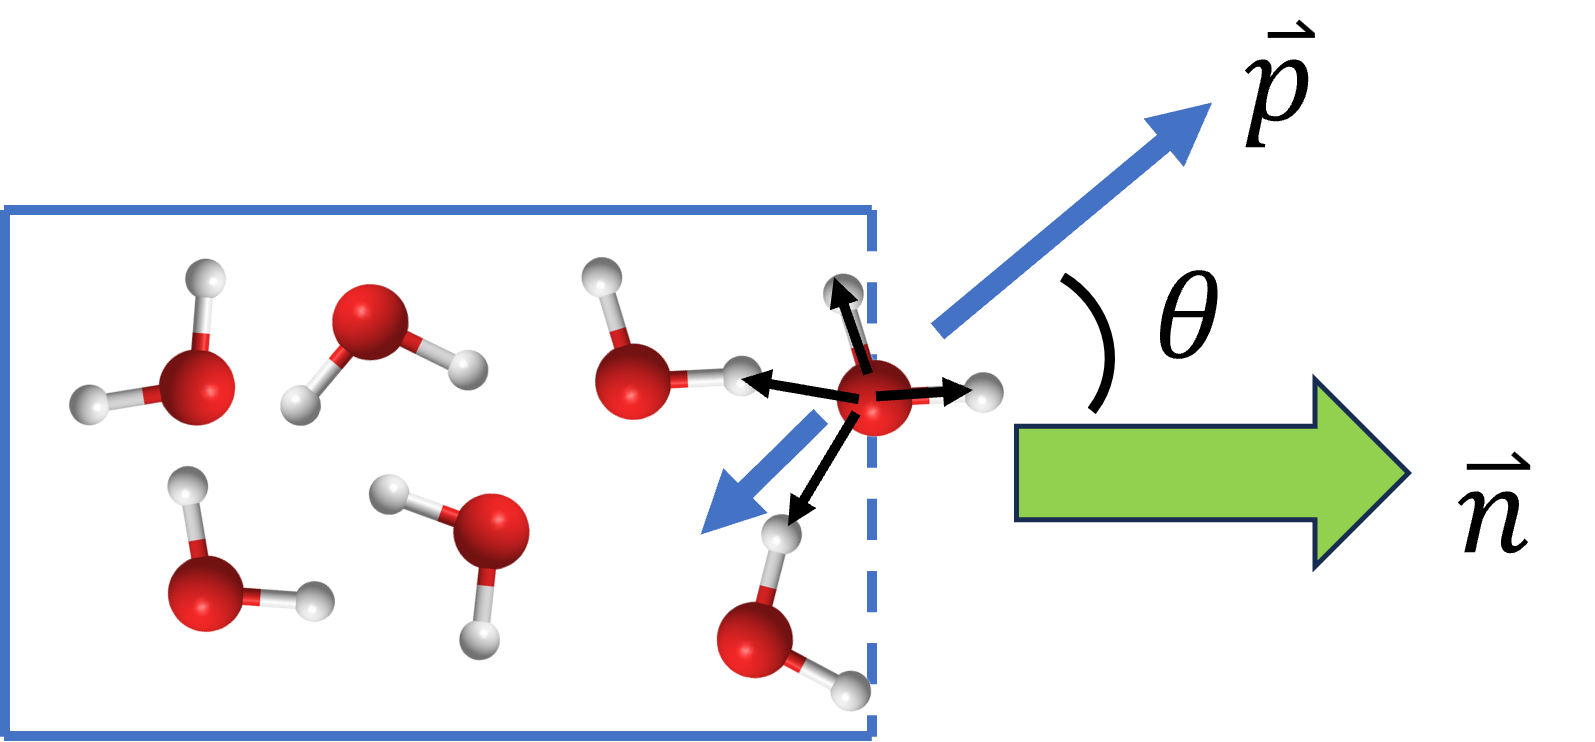
\includegraphics[width=0.9\textwidth]{images/dipole_scheme.png}
		\caption{}
		\label{fig:dipole_scheme}
	\end{subfigure}
	\hfill
	\begin{subfigure}{0.47\textwidth}
		\centering

		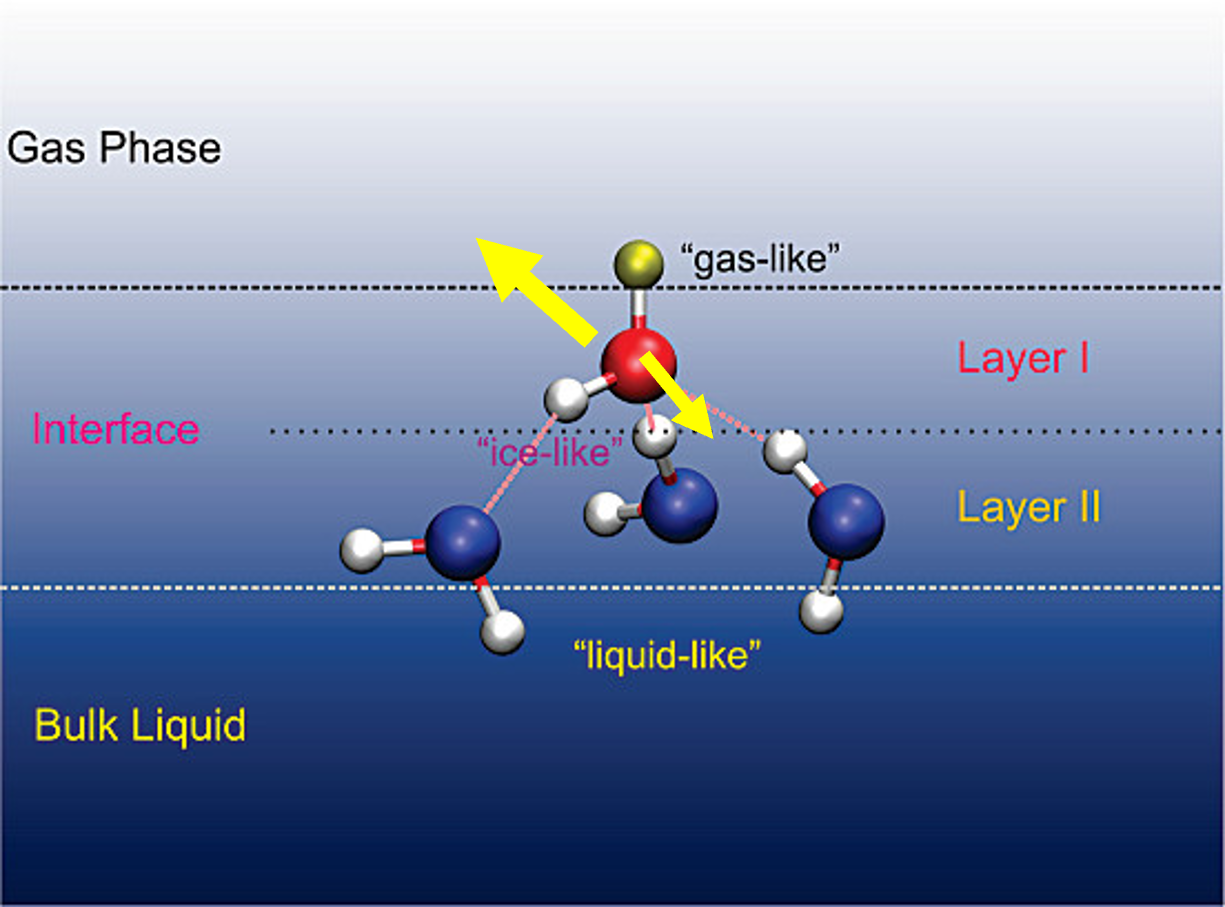
\includegraphics[width=0.9\textwidth]{images/dipole_expt.png}
		\caption{}
		\label{fig:dipole_expt}
	\end{subfigure}
	\caption{  Schematic diagram of the (a) dipole moment orientation and
		(b)		existence of two layers in the interface
		\cite{fan2009structure}.}
	\label{fig:dipole_guide}
\end{figure}

\begin{figure}[tbhp!]
	\centering
	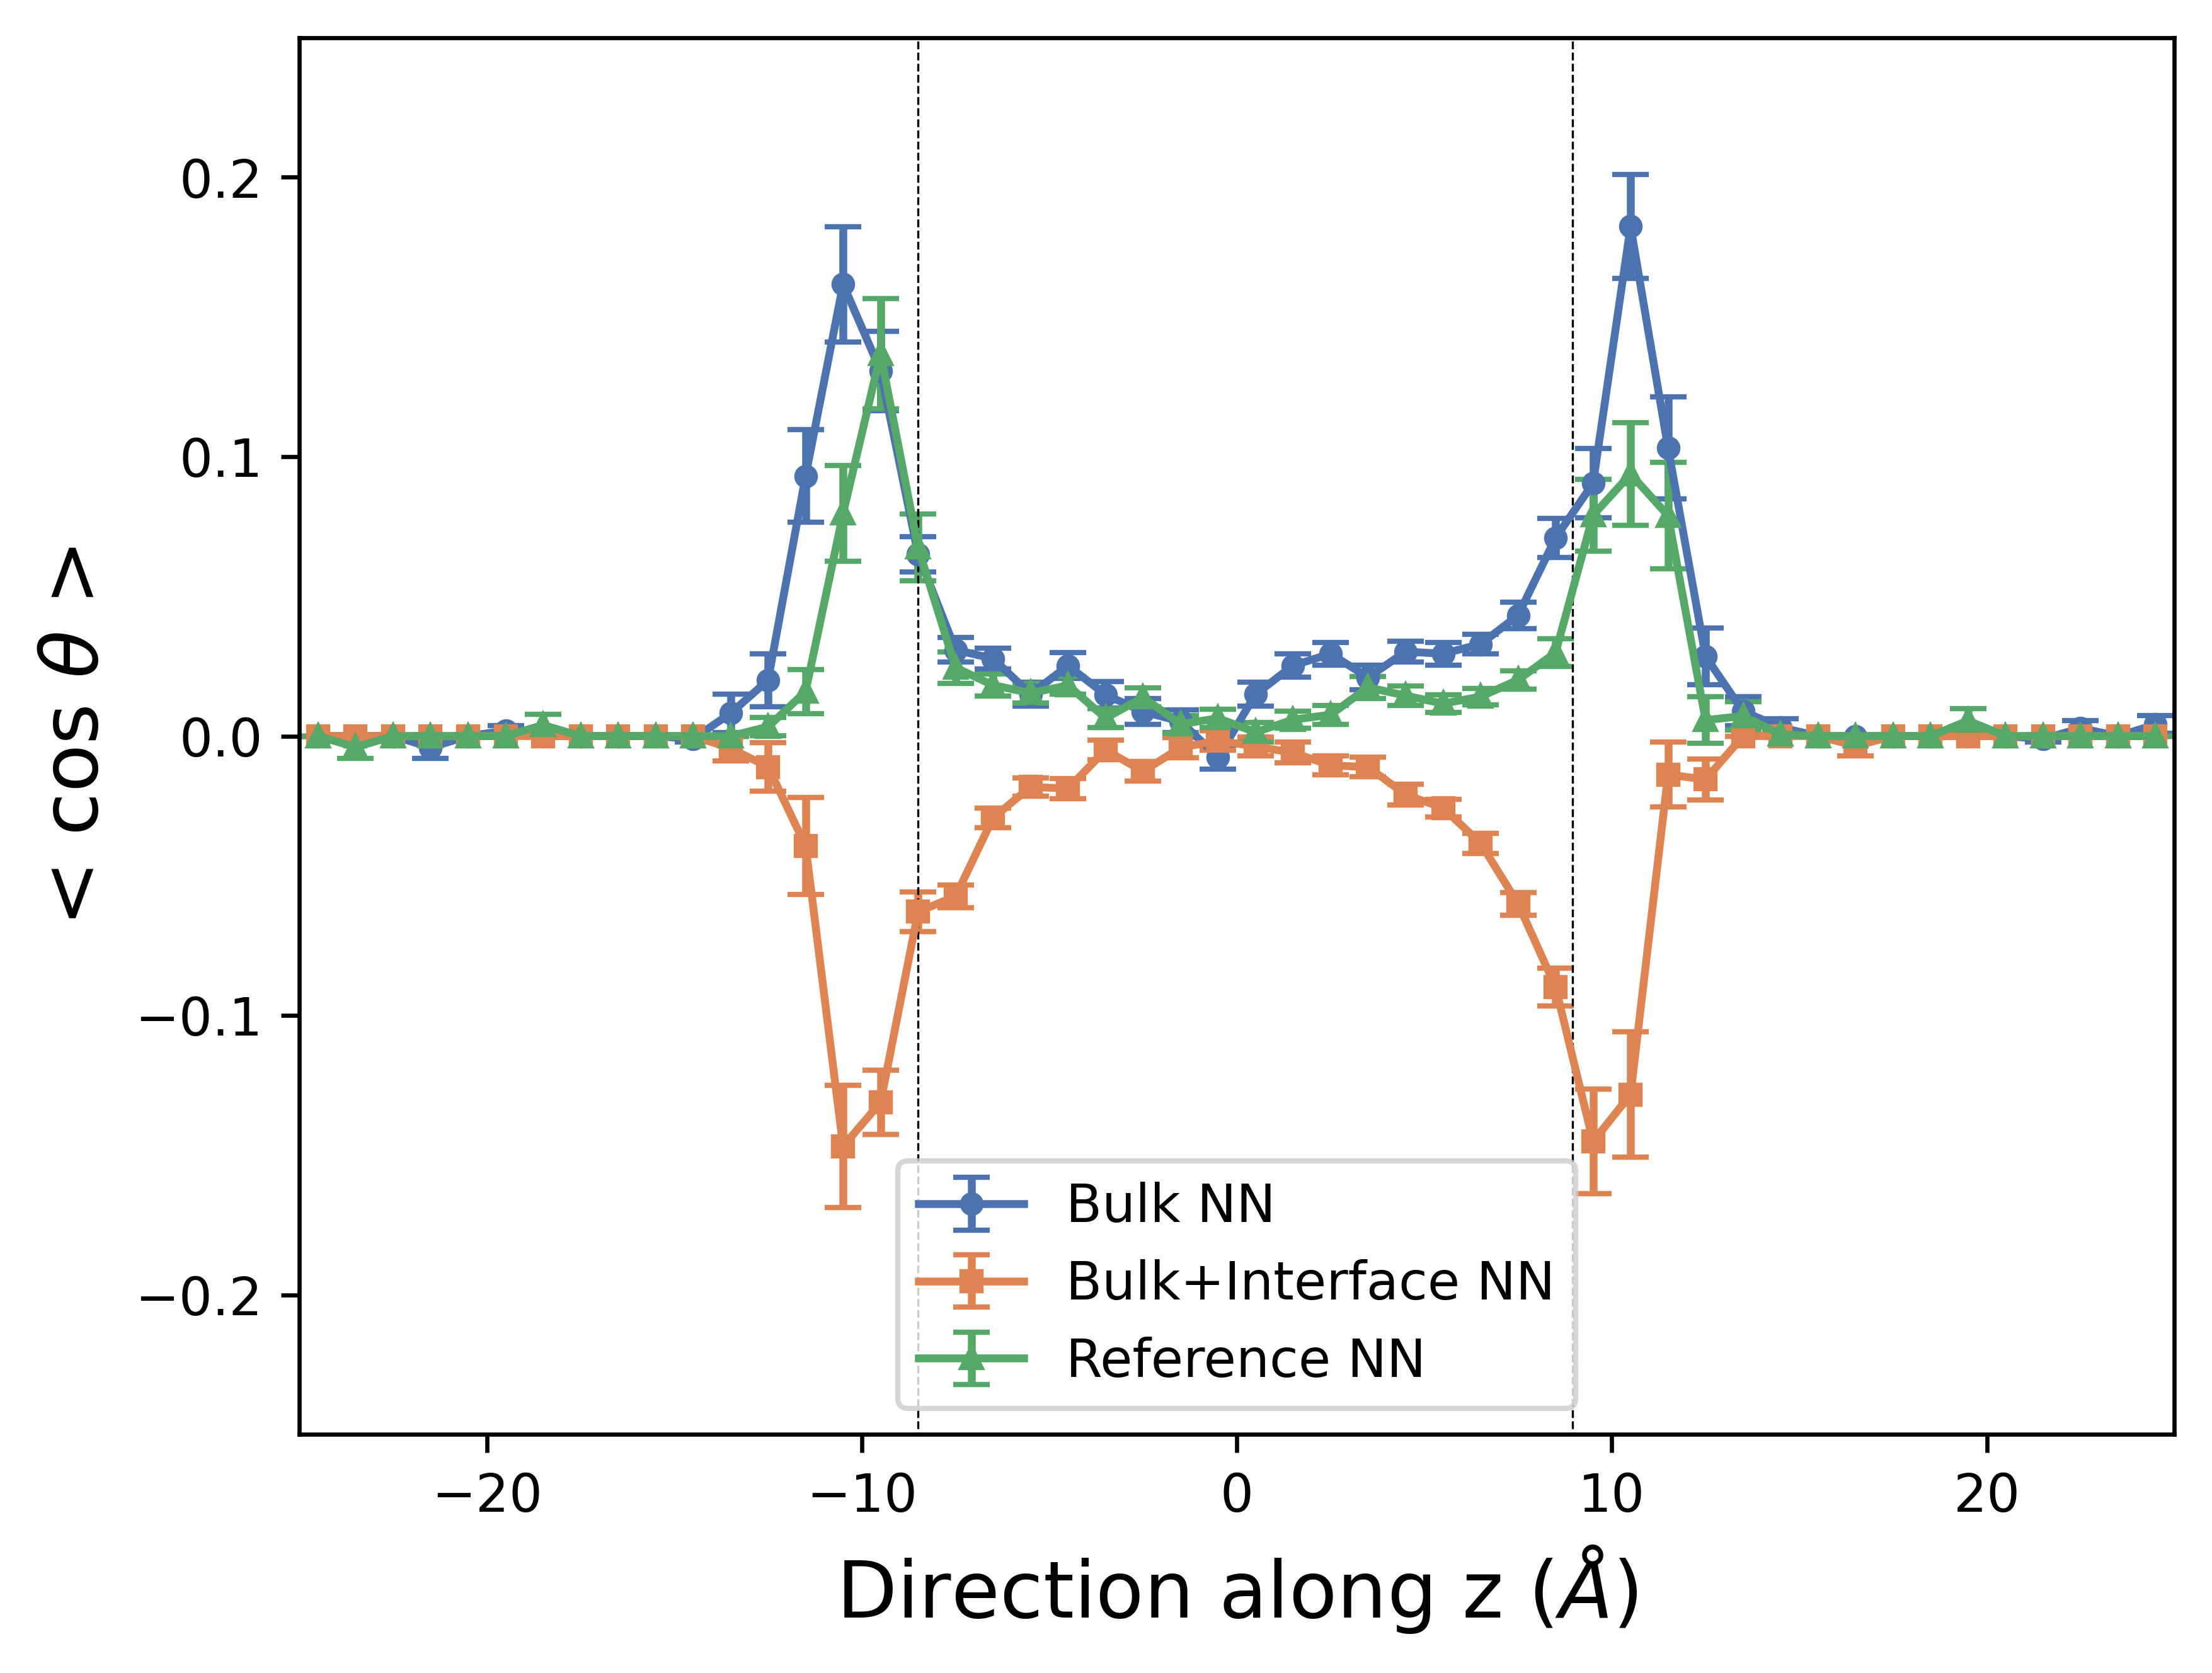
\includegraphics[width=0.75\linewidth]{images/dipole_dist_new.png}
	\caption{Dipole Orientation for different NN models. The outward normal
		vector was set along +z axis for both the top and bottom
		surface. The vertical
		lines
		are
		the Gibbs Dividing Surface in which the density is half of the
		bulk value.
	}
	\label{fig:dipole_orient}
\end{figure}


\clearpage

\chapter{Conclusion and Future Work}

In this thesis, we generated a deep neural network potential and assess its
predictability in obtaining relevant system properties such as density, surface
tension, and dipole orientation. Due to numerical instabilities using SCAN functional for interfaces, we used instead  similar  but accurate and numerically efficient regularized-restored r$^2$SCAN functional. Neural network potential trained on only bulk
systems did not perform well when used on trajectories containing interfaces.
Specifically, it predicted very underestimated values of surface tension and
slightly underestimated bulk density. Adding interface dataset to the training
did improve the prediction of mass density and surface tension, implying that surface defects
play a role in surface properties of water. In addition, the bulk+interface trained NNP have the same accuracy as the reference NNP used but with smaller training dataset. In all the models, they fail to describe microscopic properties such as dipole orientation at the surface but still obtain good macroscopic properties.

This study should be extended by training the deep neural network model for large system size as to take into account finite size effects. Moreover, it would be interesting to study how initial parameters such as virial when included in the training will affect the results of this thesis. Also, long-range electrostatic interactions play a major role in obtaining accurate molecular dipolar fluctuations and should be included during training. Ultimately, the accuracy of the deep neural network potential is always intertwined to the DFT accuracy used. Hence, a better exchange-correlation functional or pseudopotential should improve the physics of many body systems.


\printbibliography[heading=bibintoc]
% \addcontentsline{toc}{chapter}{Bibliography}
\chapter*{Appendix}

\renewcommand{\thefigure}{A.\arabic{figure}}
\setcounter{figure}{0}

\begin{figure}[h!]
    \centering

    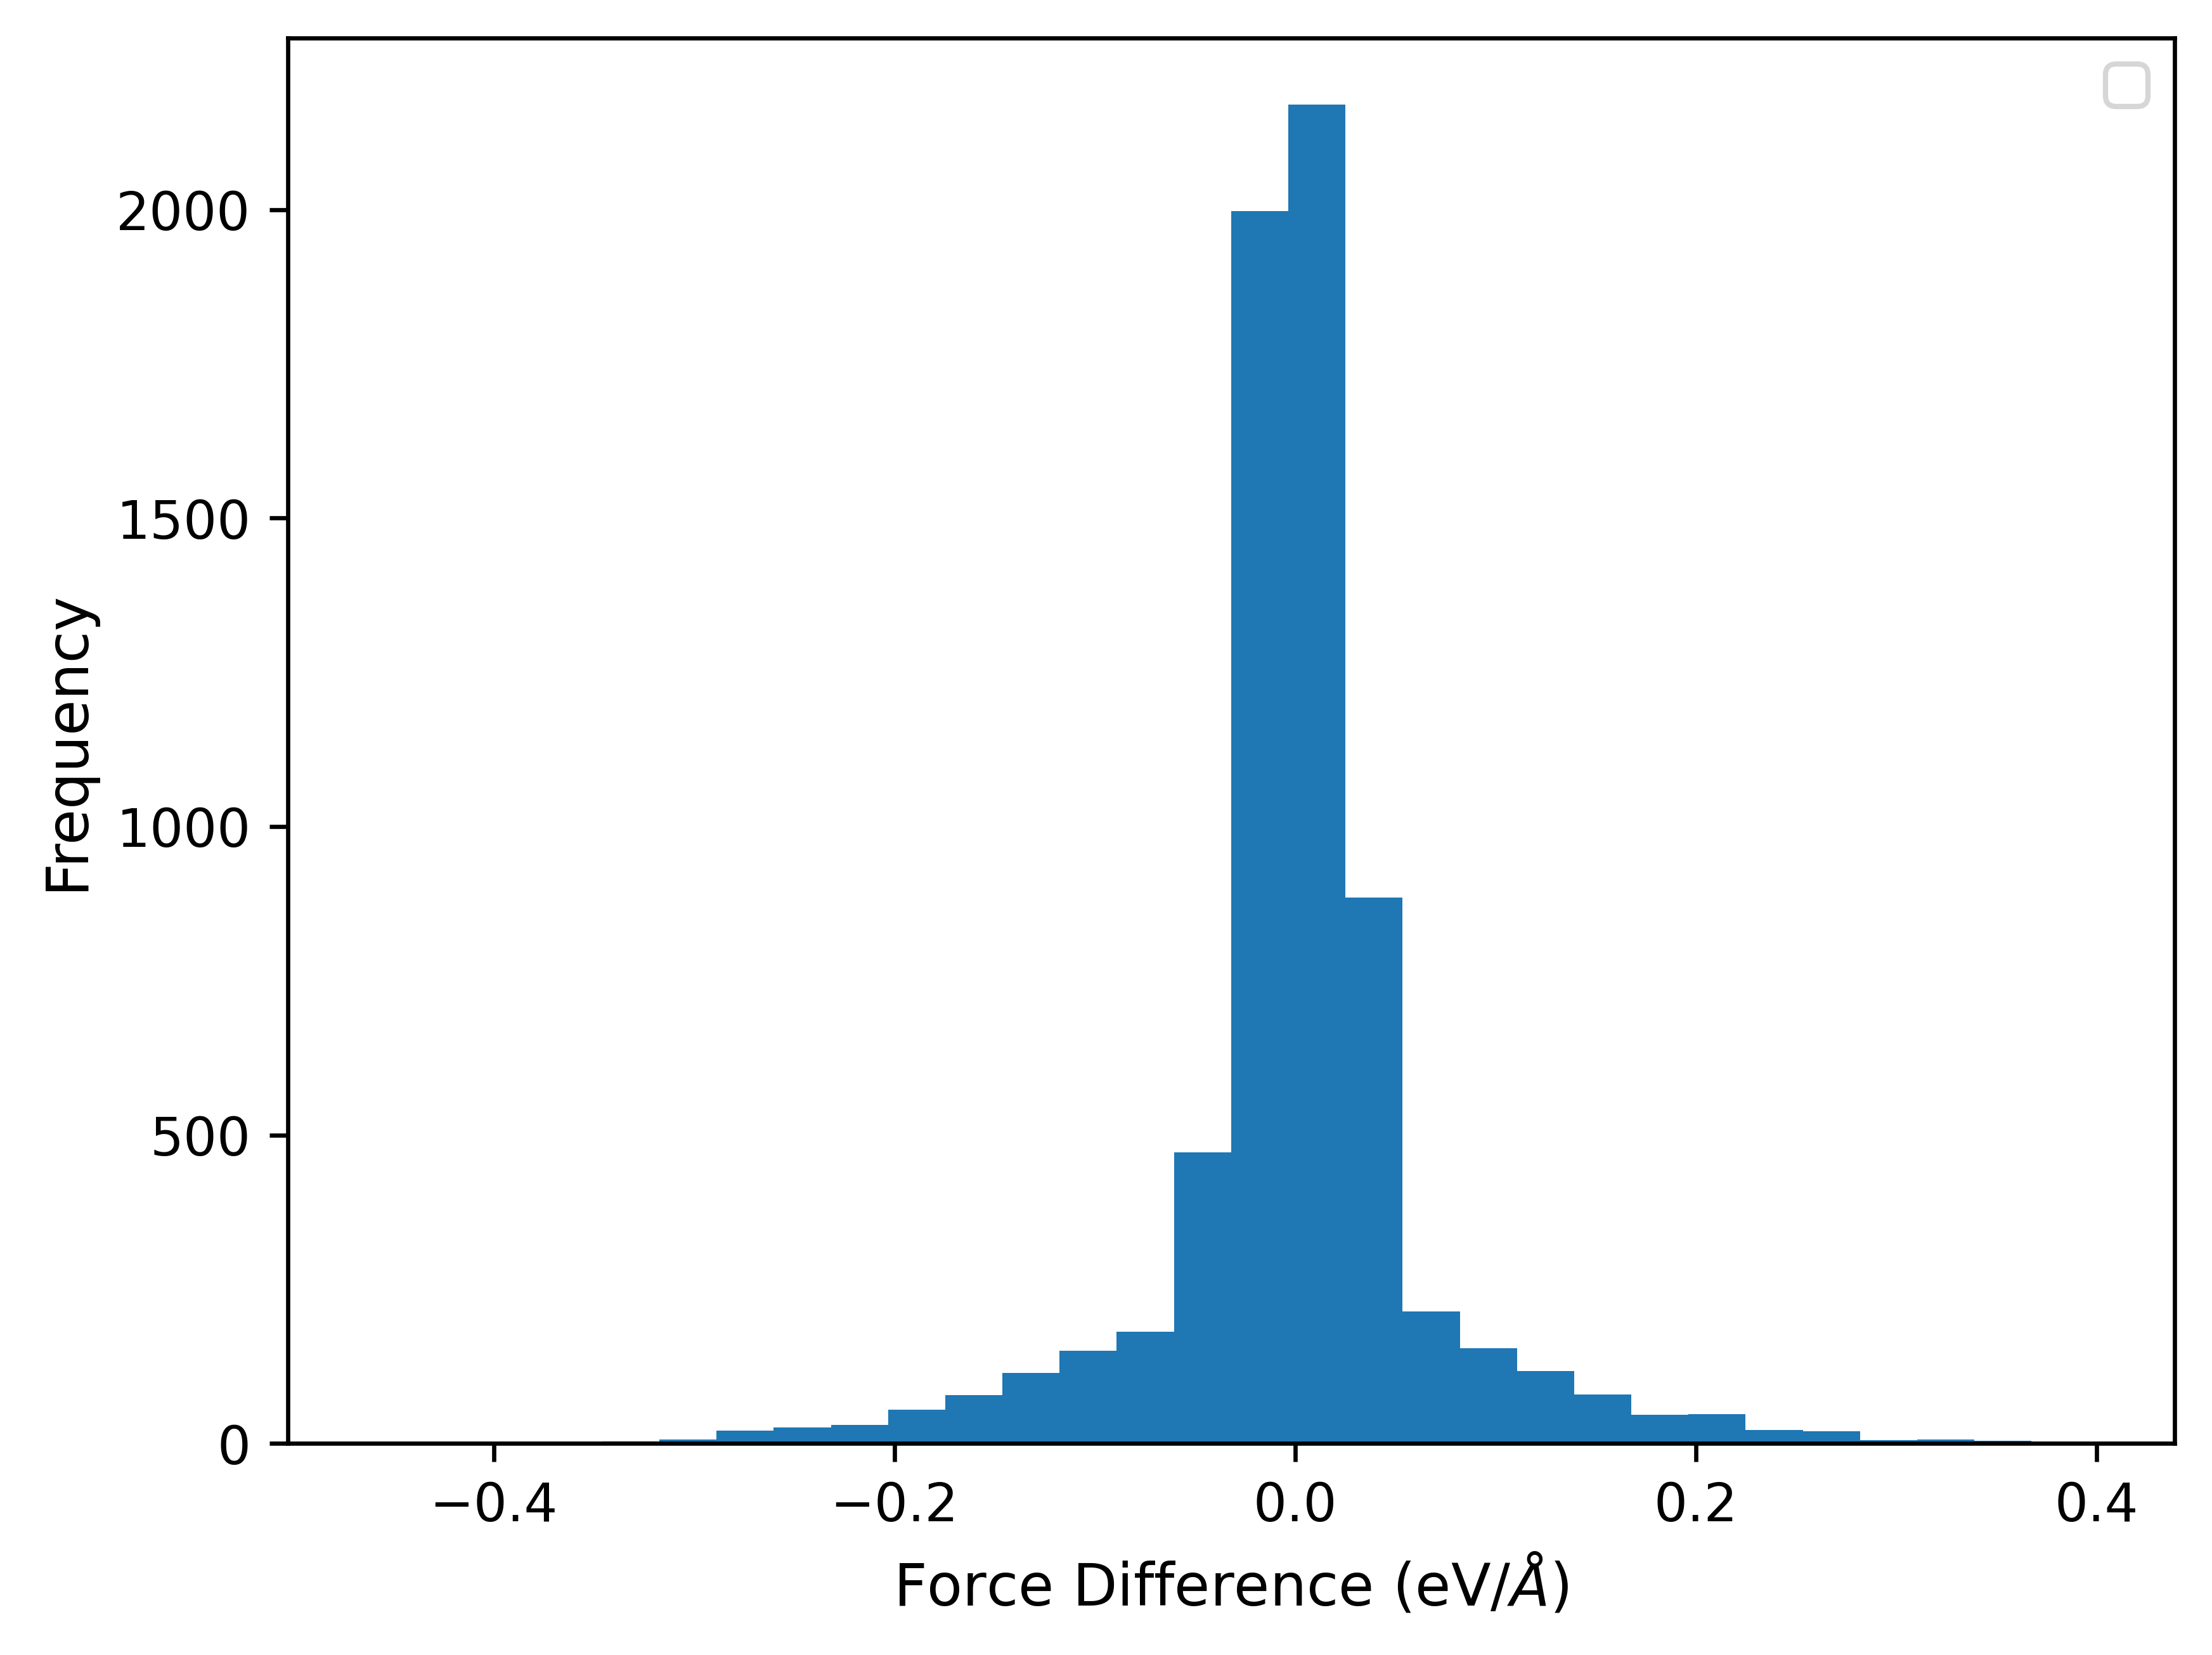
\includegraphics[width=0.7\linewidth]{images/scan_vs_r2scan/r2scan_hist_force.png}
    \caption{Distribution of the error on forces between SCAN and r2SCAN
        functional.
    }
    \label{fig:scan_r2scan_F_dist}
\end{figure}

\begin{figure}[tbhp]
    \centering
    \begin{subfigure}{0.32\textwidth}
        \centering
        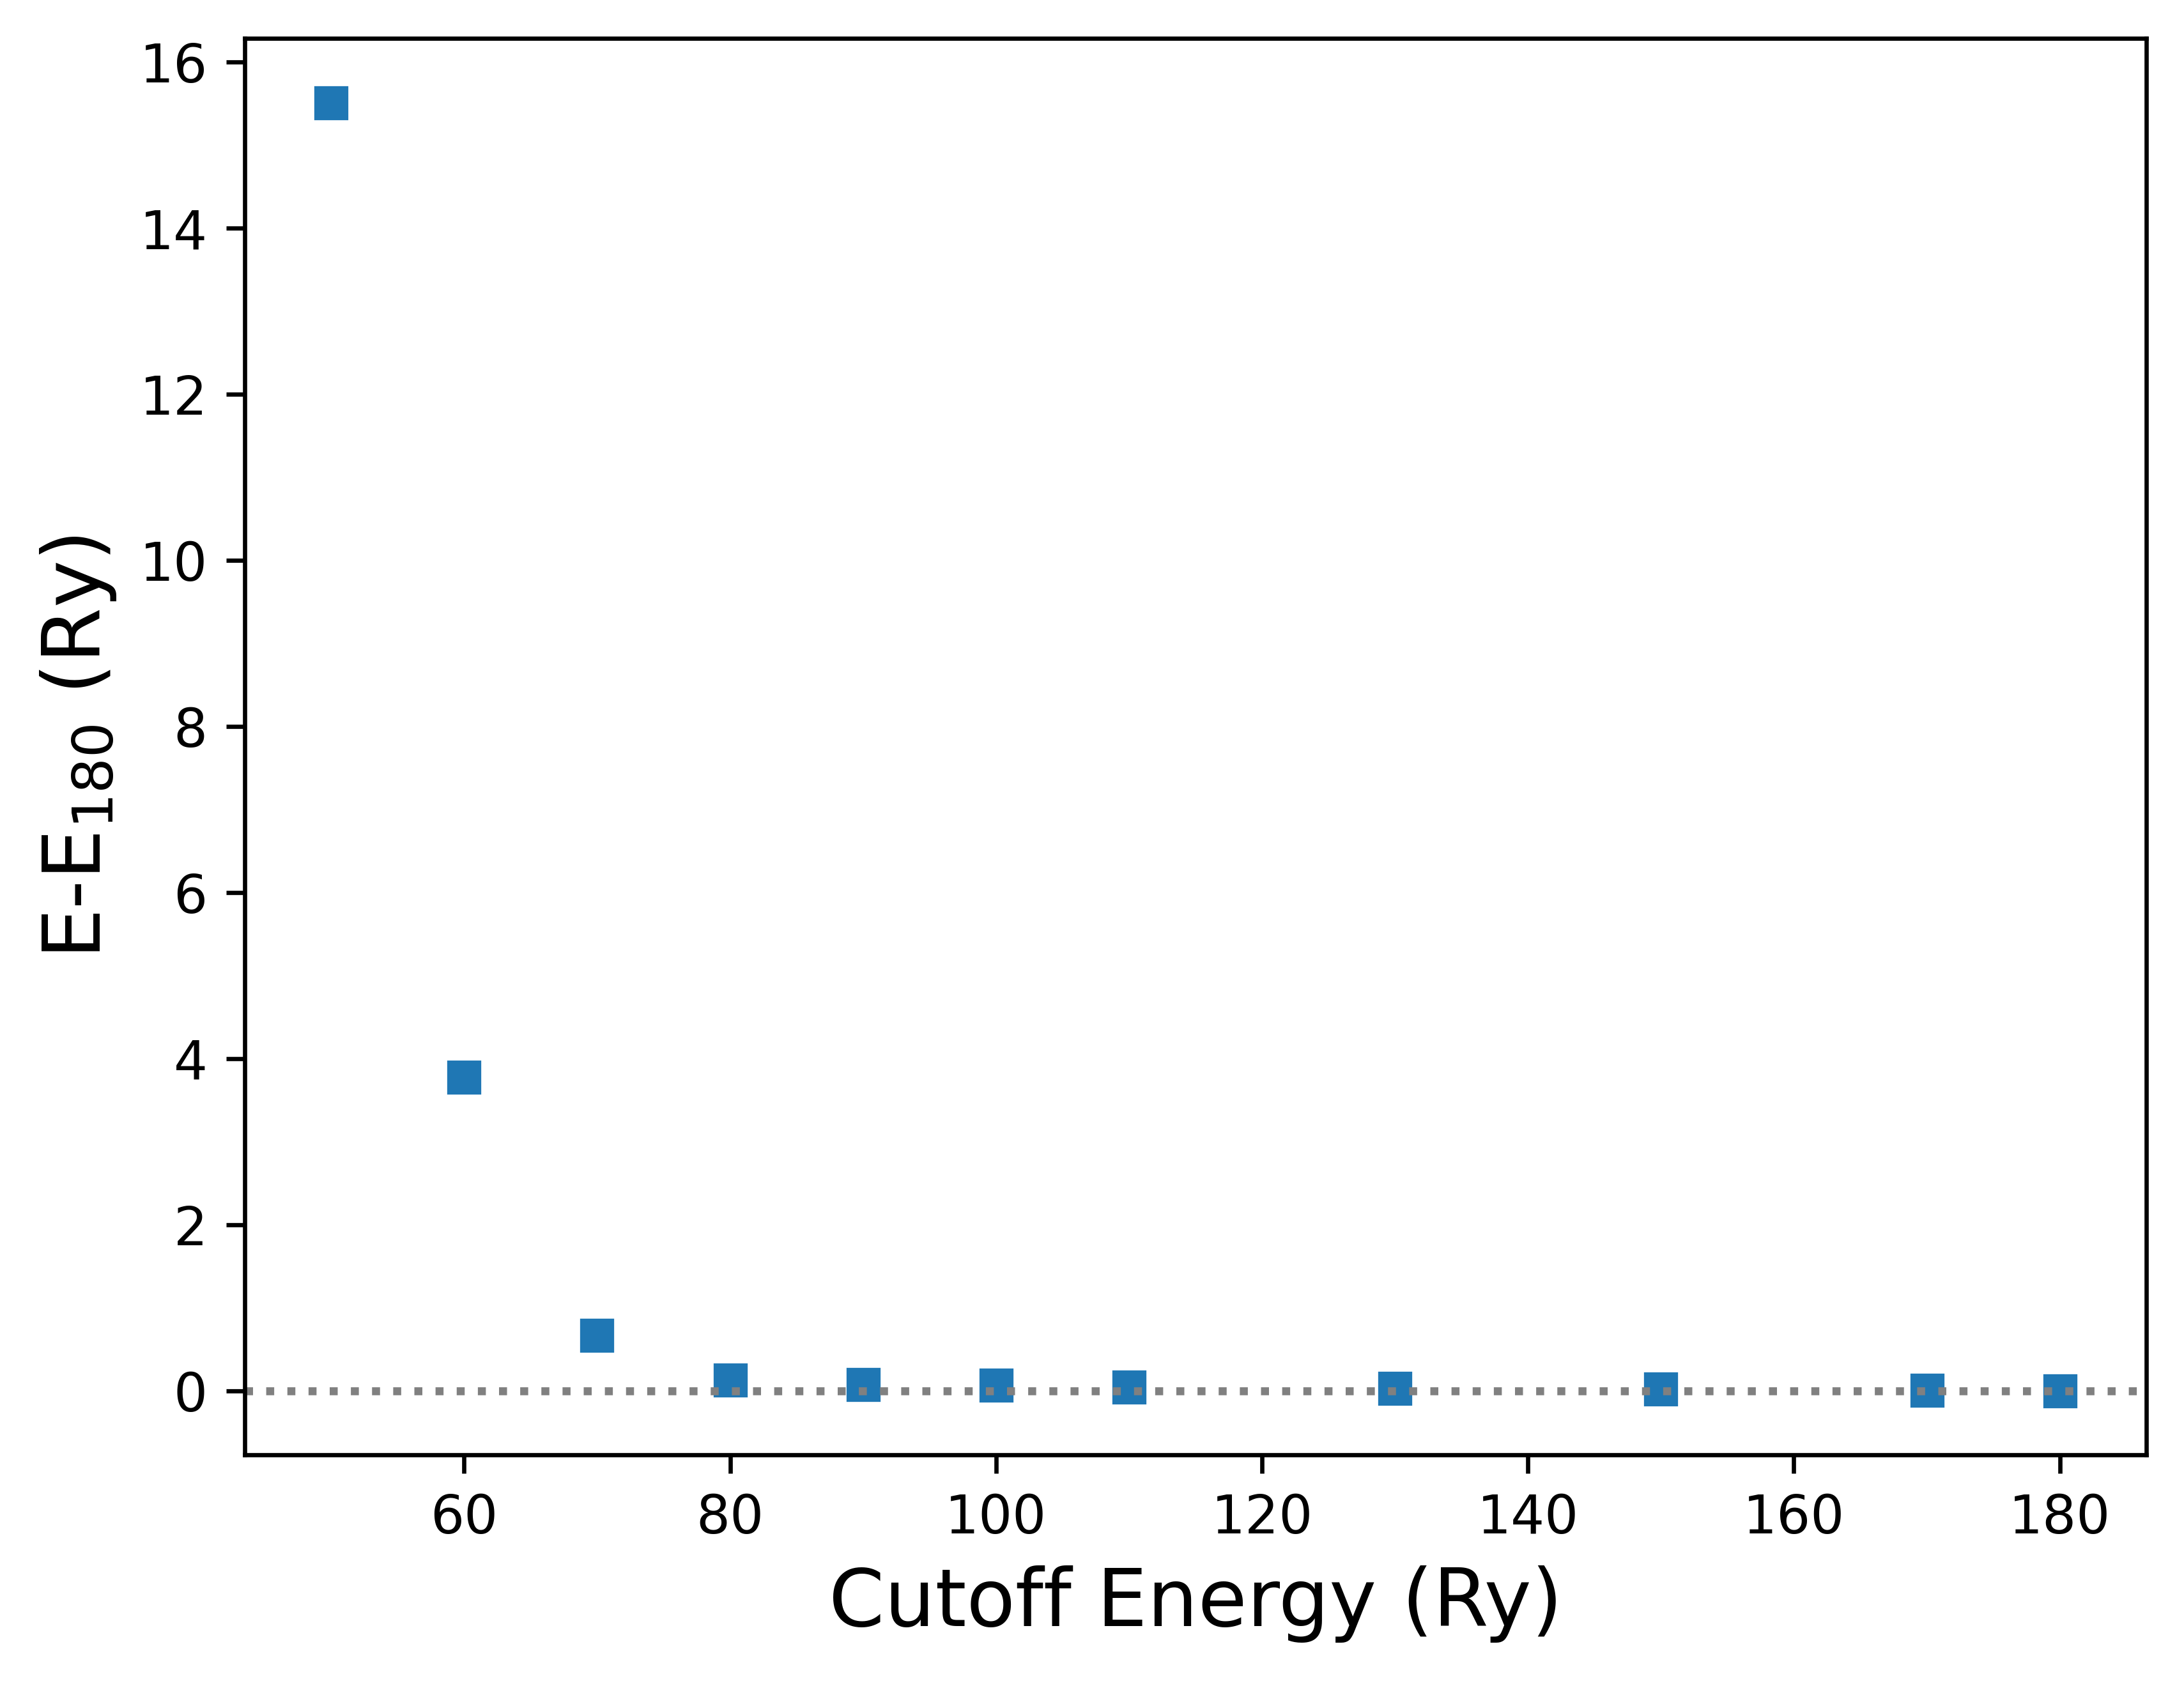
\includegraphics[width=1\textwidth]{convergence/SCAN/conv-energy.png}
        \caption{}
        % \label{fig:}
    \end{subfigure}
    \hfill
    \begin{subfigure}{0.32\textwidth}
        \centering
        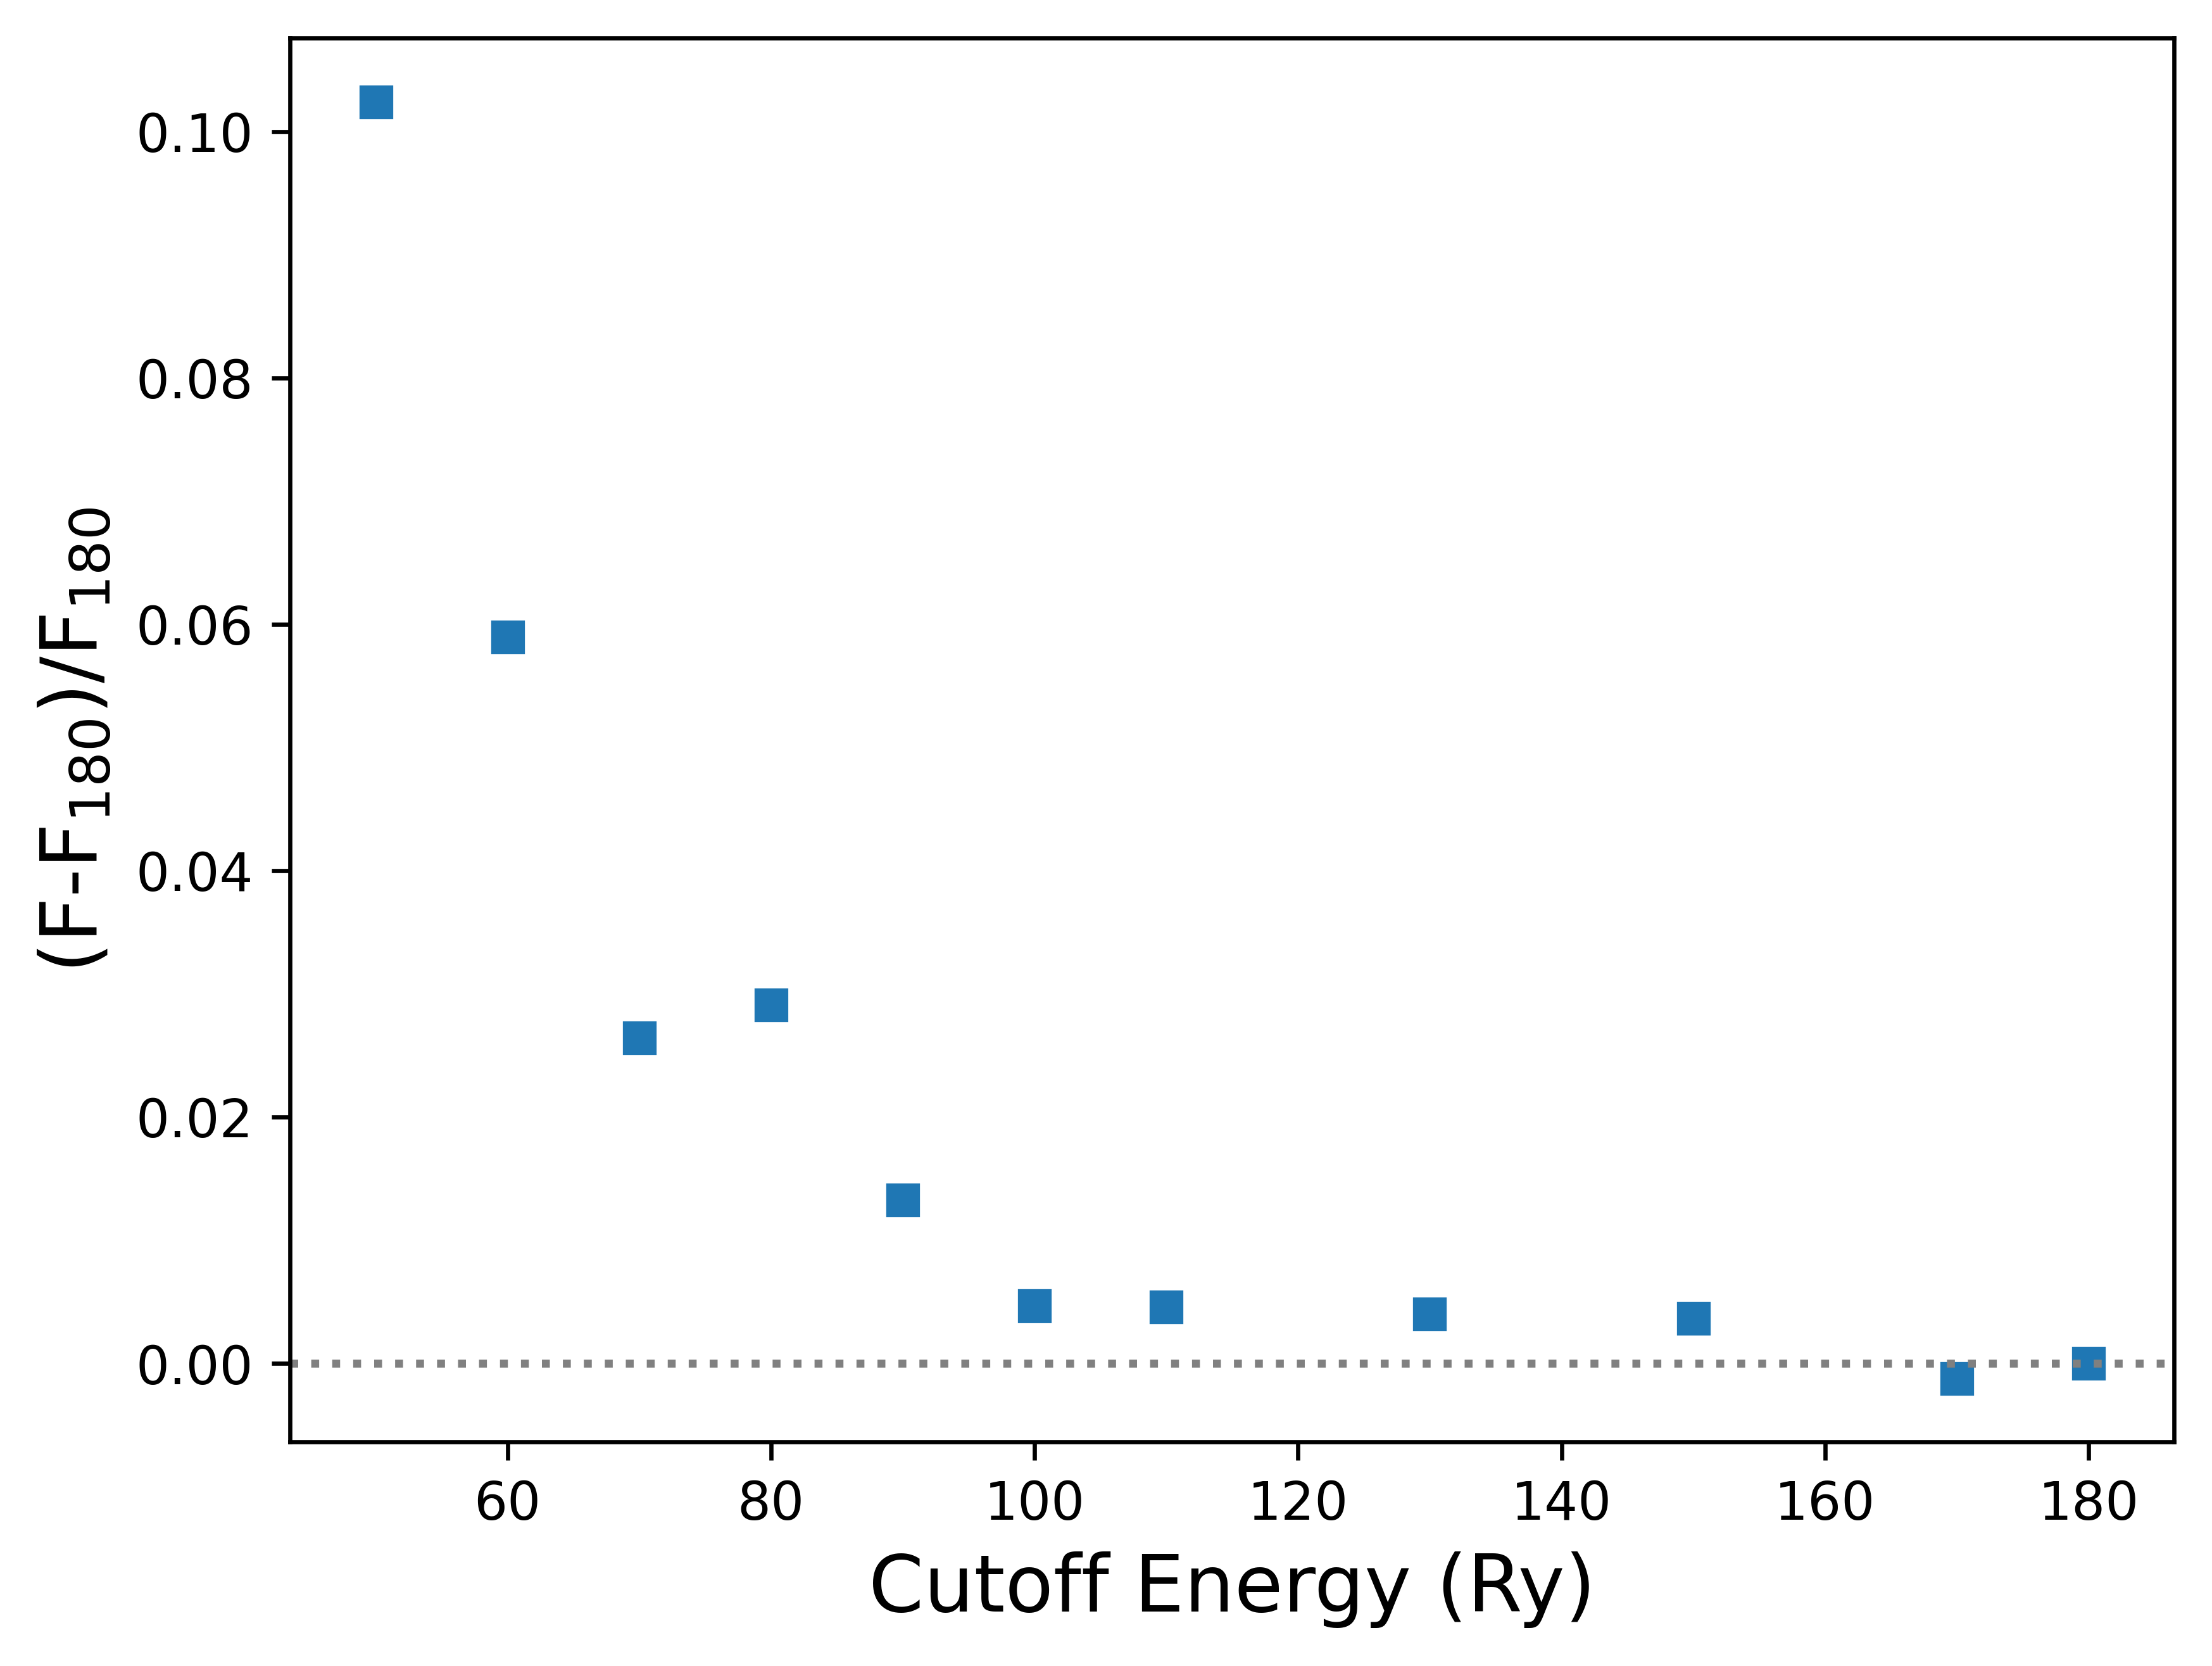
\includegraphics[width=1\textwidth]{convergence/SCAN/conv-force.png}
        \caption{}
        % \label{fig:}
    \end{subfigure}
    \hfill
    \begin{subfigure}{0.32\textwidth}
        \centering

        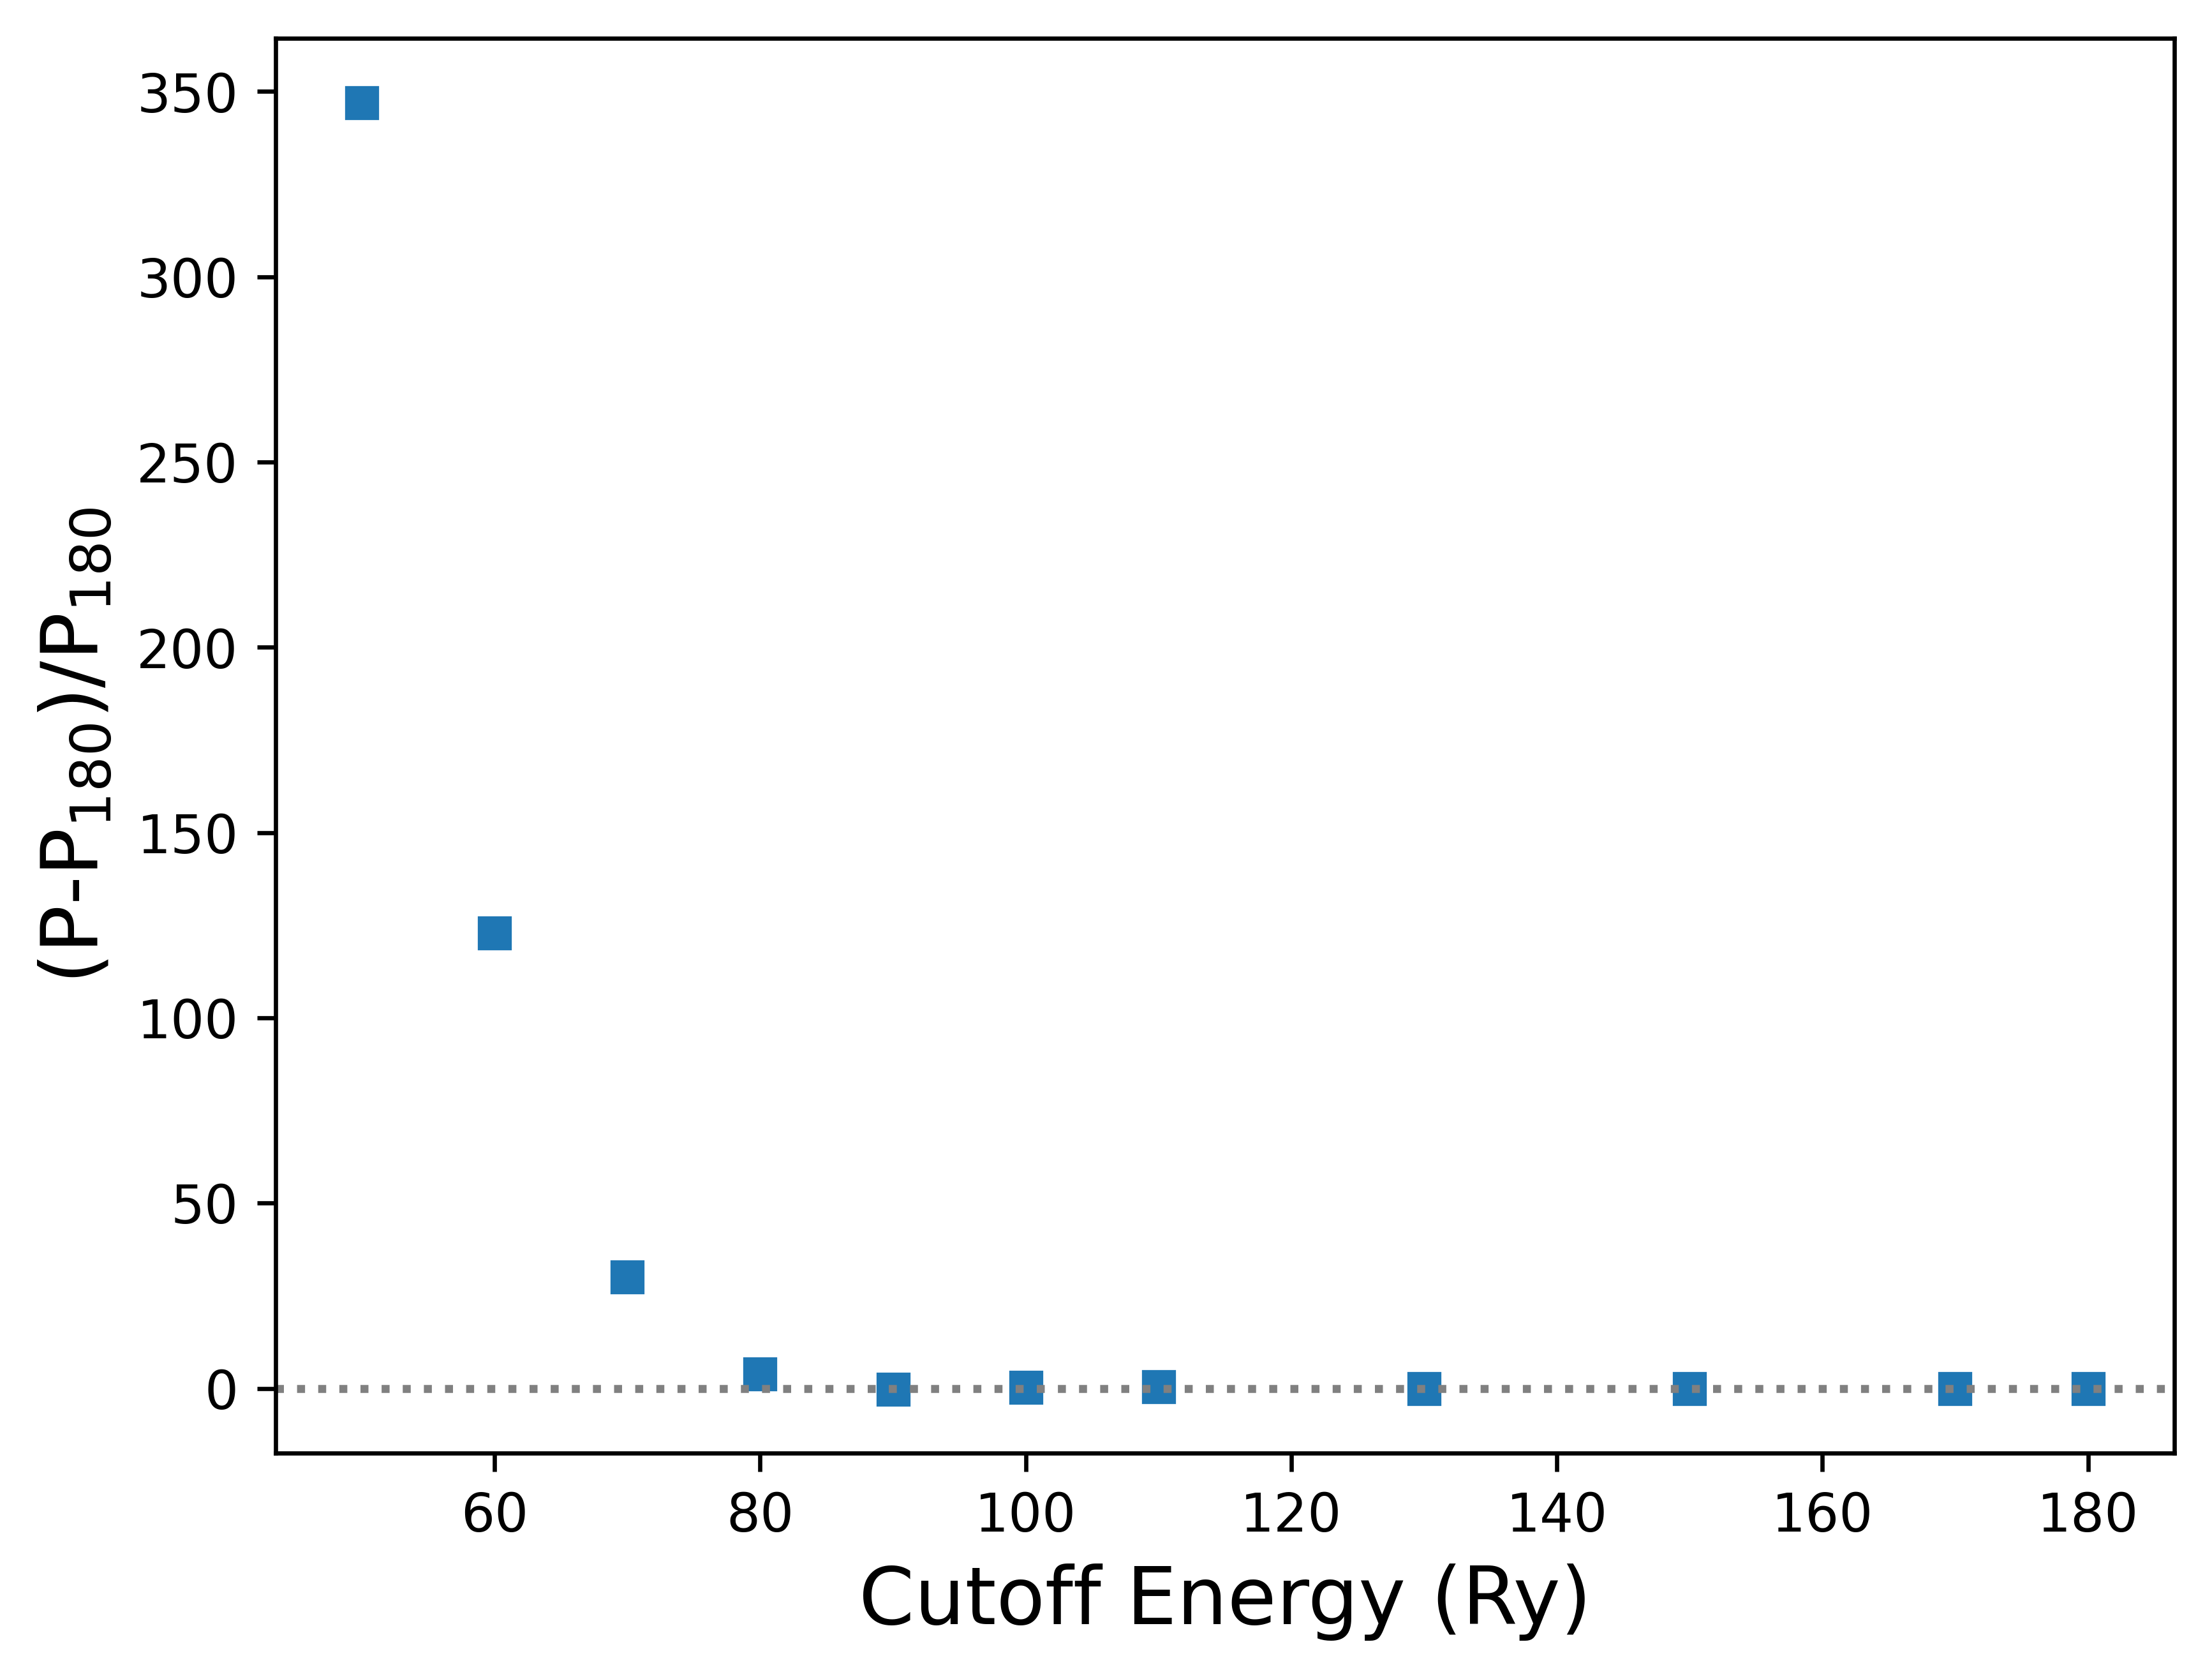
\includegraphics[width=1\textwidth]{convergence/SCAN/conv-pressure.png}
        \caption{}
        % \label{fig:}
    \end{subfigure}
    \caption{Convergence tests using the SCAN functional on (a) total energy,
        (b) total force, and (c) total pressure. All values are shifted
        with respect to the reference value at 180 Ry. The forces and pressure
        are also normalized with the corresponding reference values at 180 Ry.}
    \label{fig:conv_scan}
\end{figure}

\begin{figure}[tbhp]
    \centering
    \begin{subfigure}{0.32\textwidth}
        \centering
        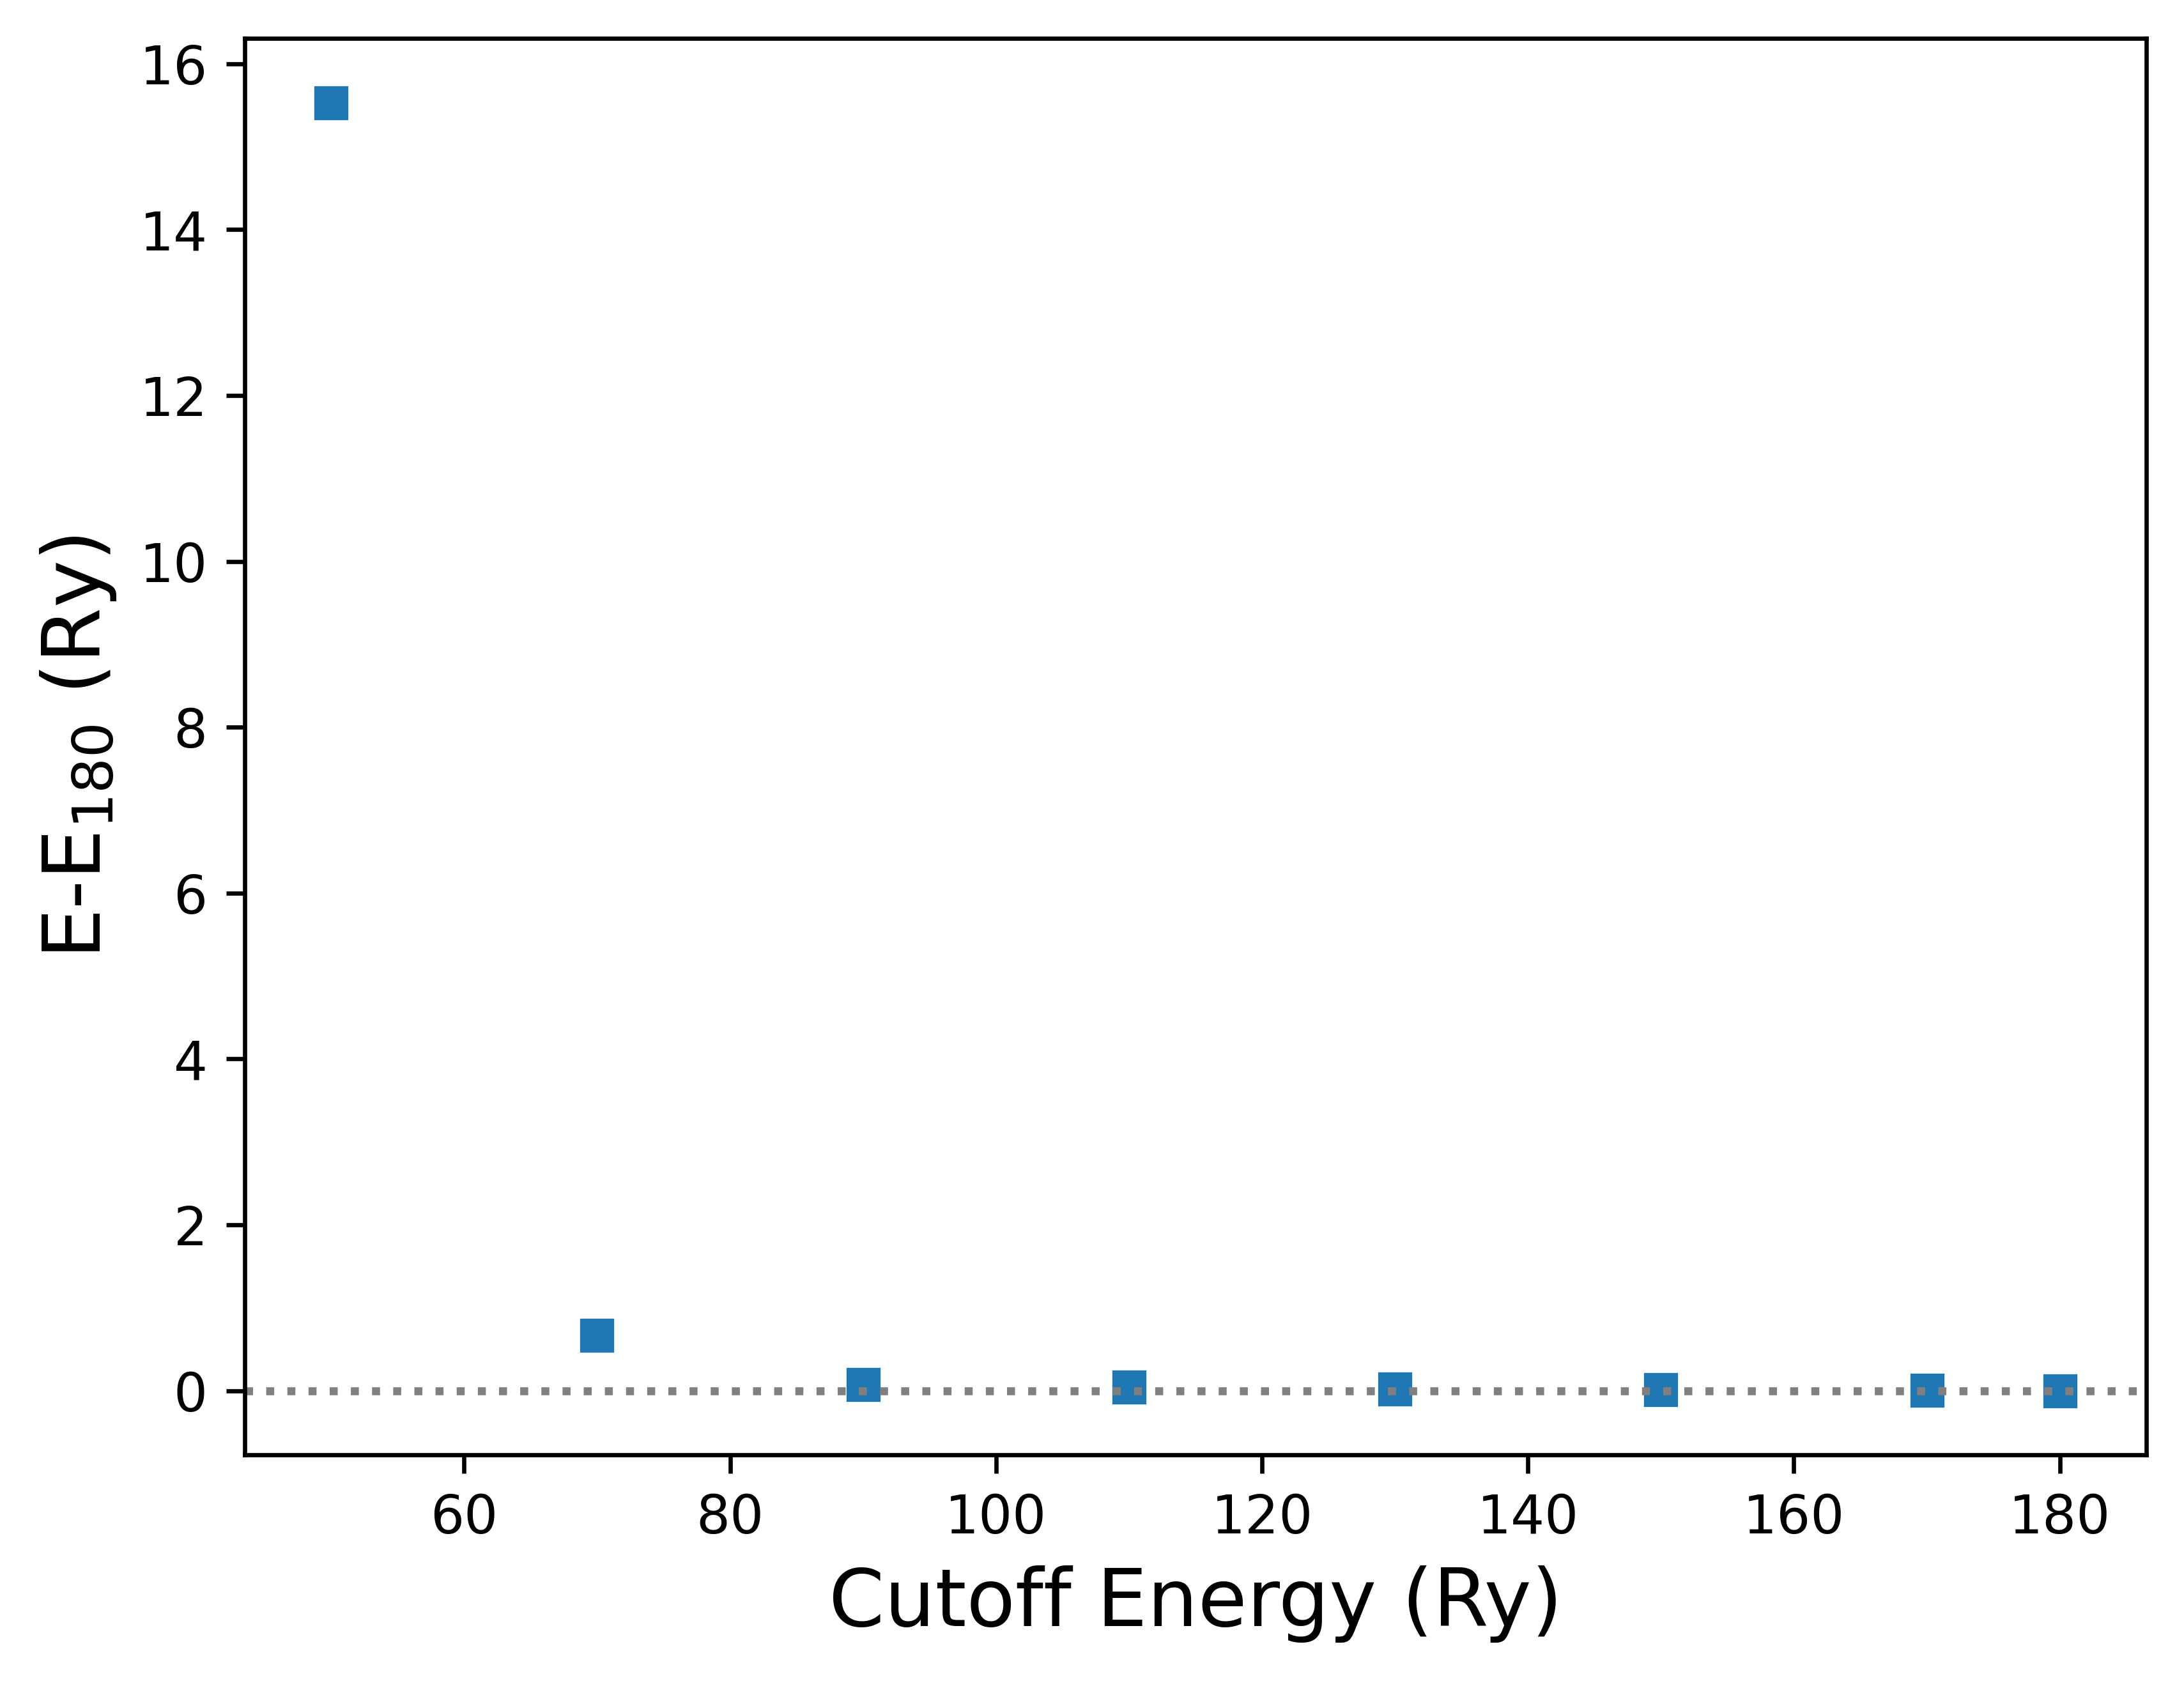
\includegraphics[width=1\textwidth]{convergence/R2SCAN/conv-energy.png}
        \caption{}
        % \label{fig:}
    \end{subfigure}
    \hfill
    \begin{subfigure}{0.32\textwidth}
        \centering
        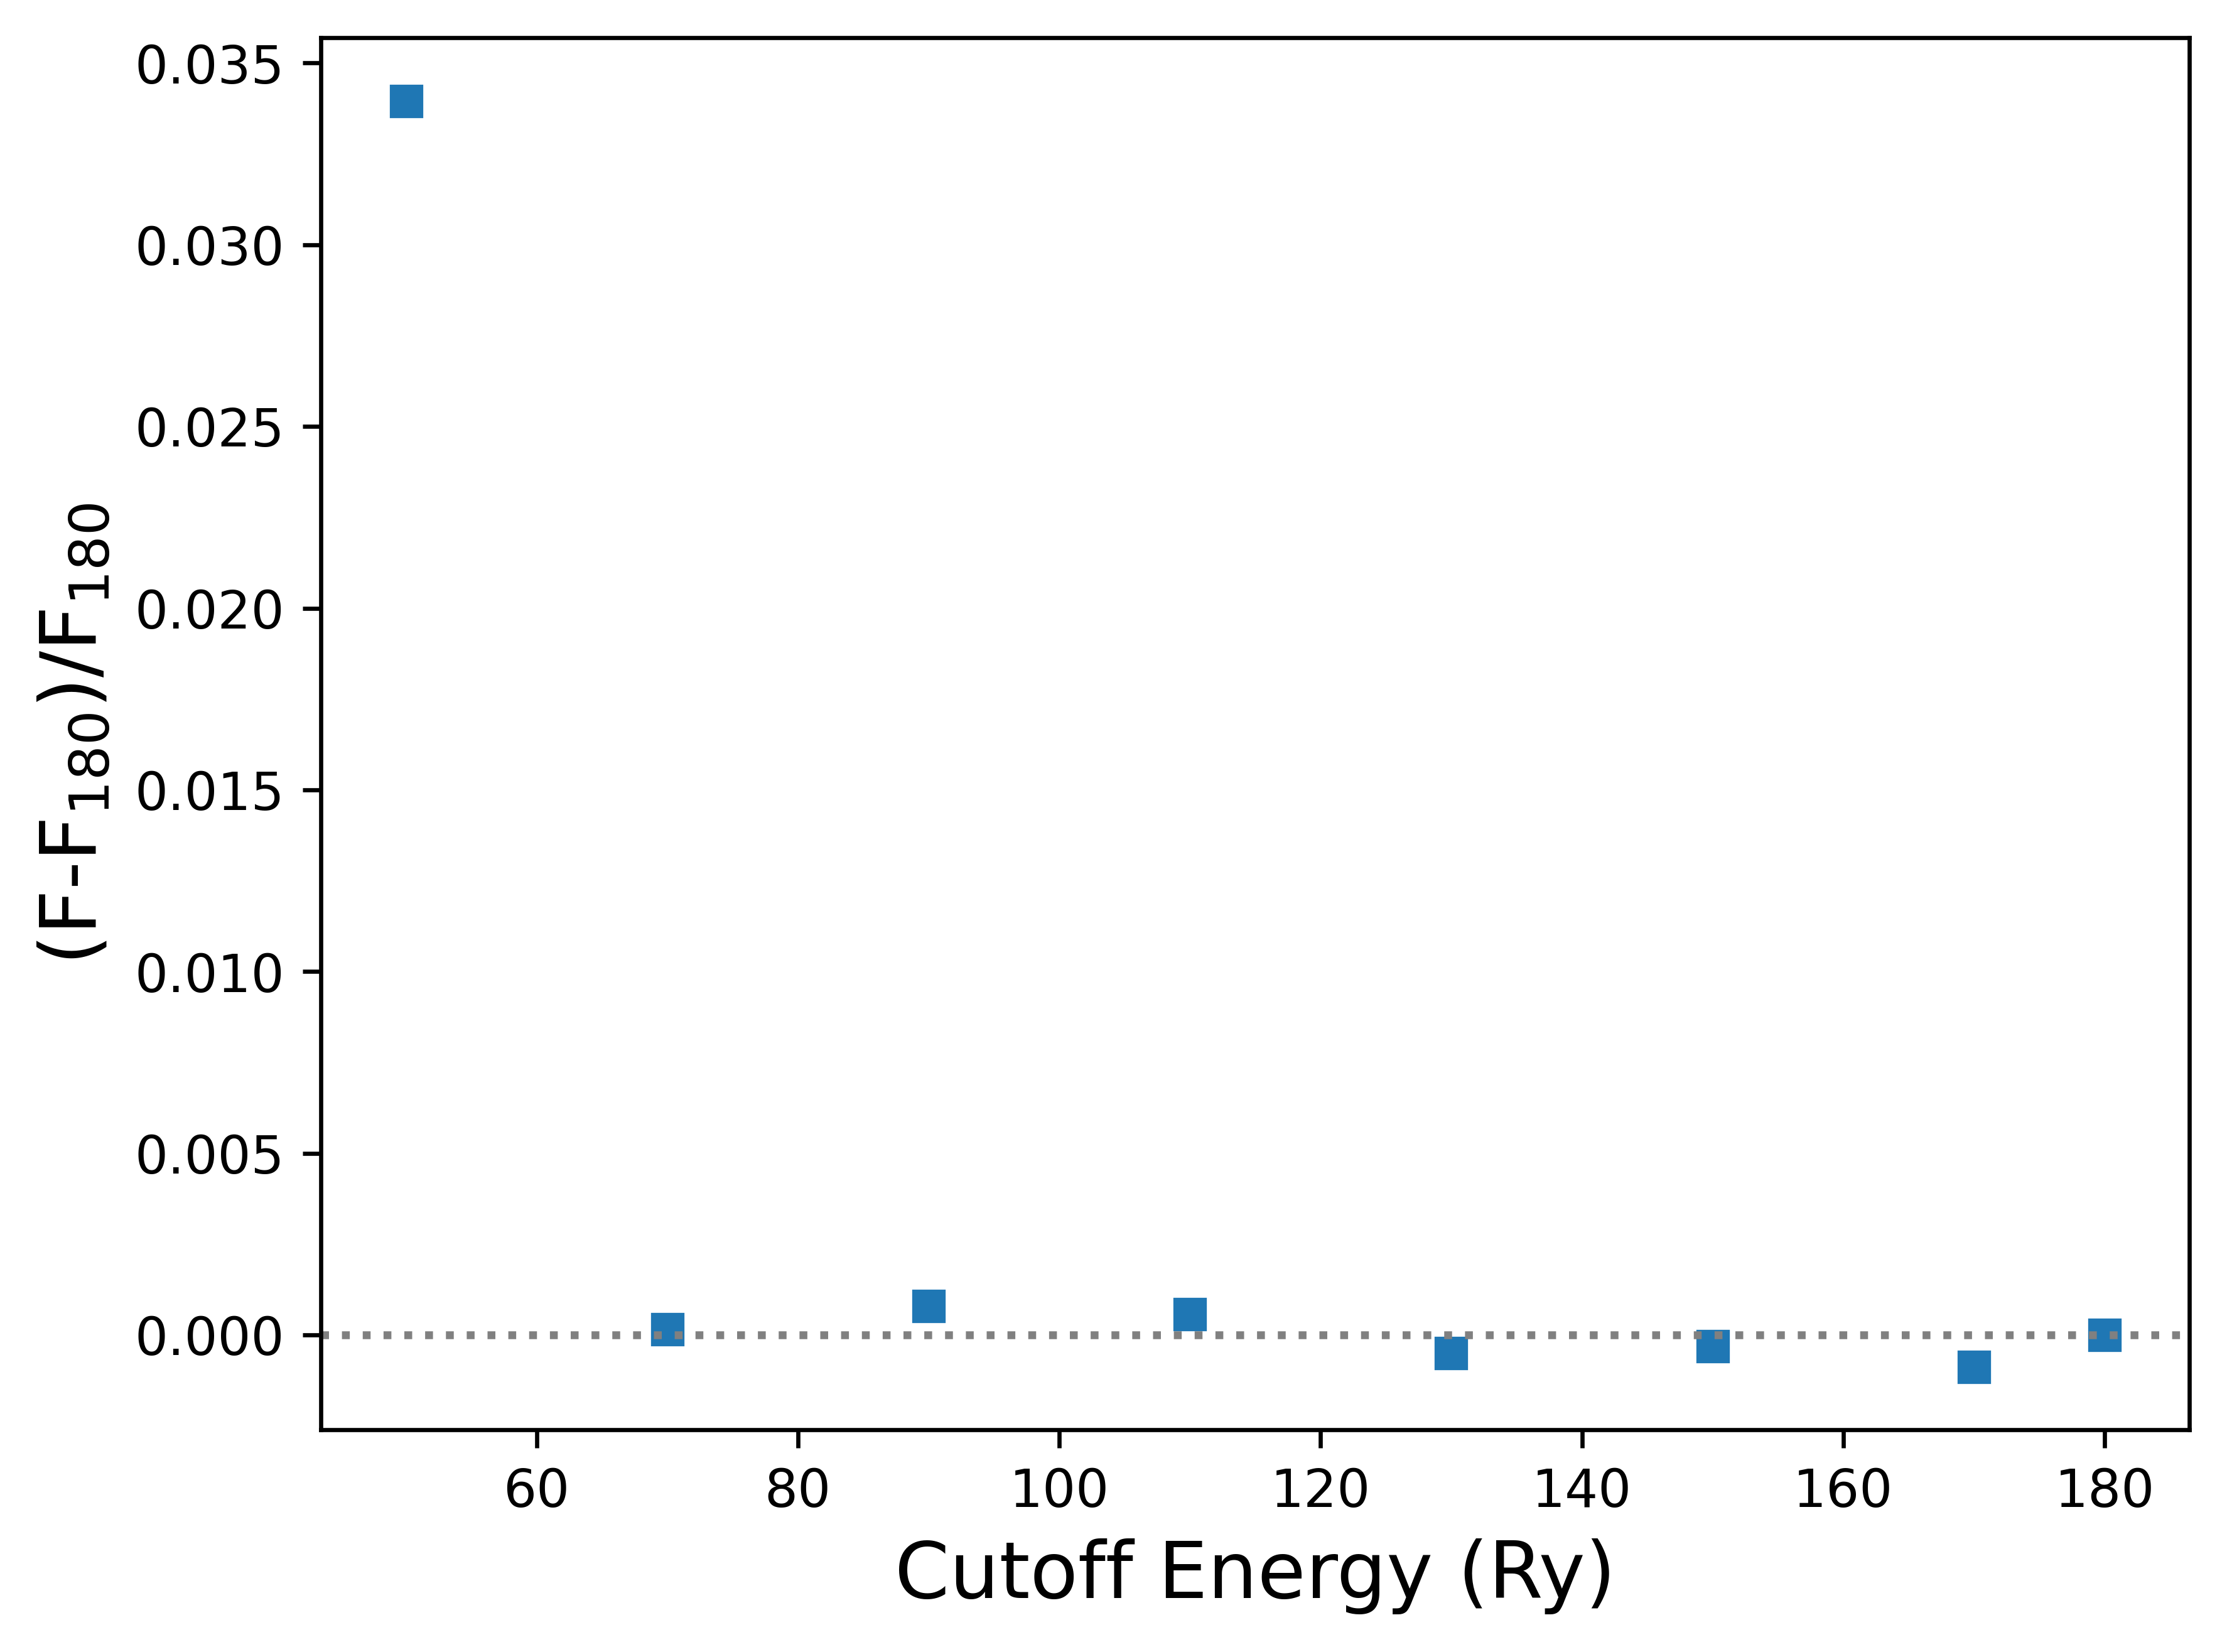
\includegraphics[width=1\textwidth]{convergence/R2SCAN/conv-force.png}
        \caption{}
        % \label{fig:}
    \end{subfigure}
    \hfill
    \begin{subfigure}{0.32\textwidth}
        \centering

        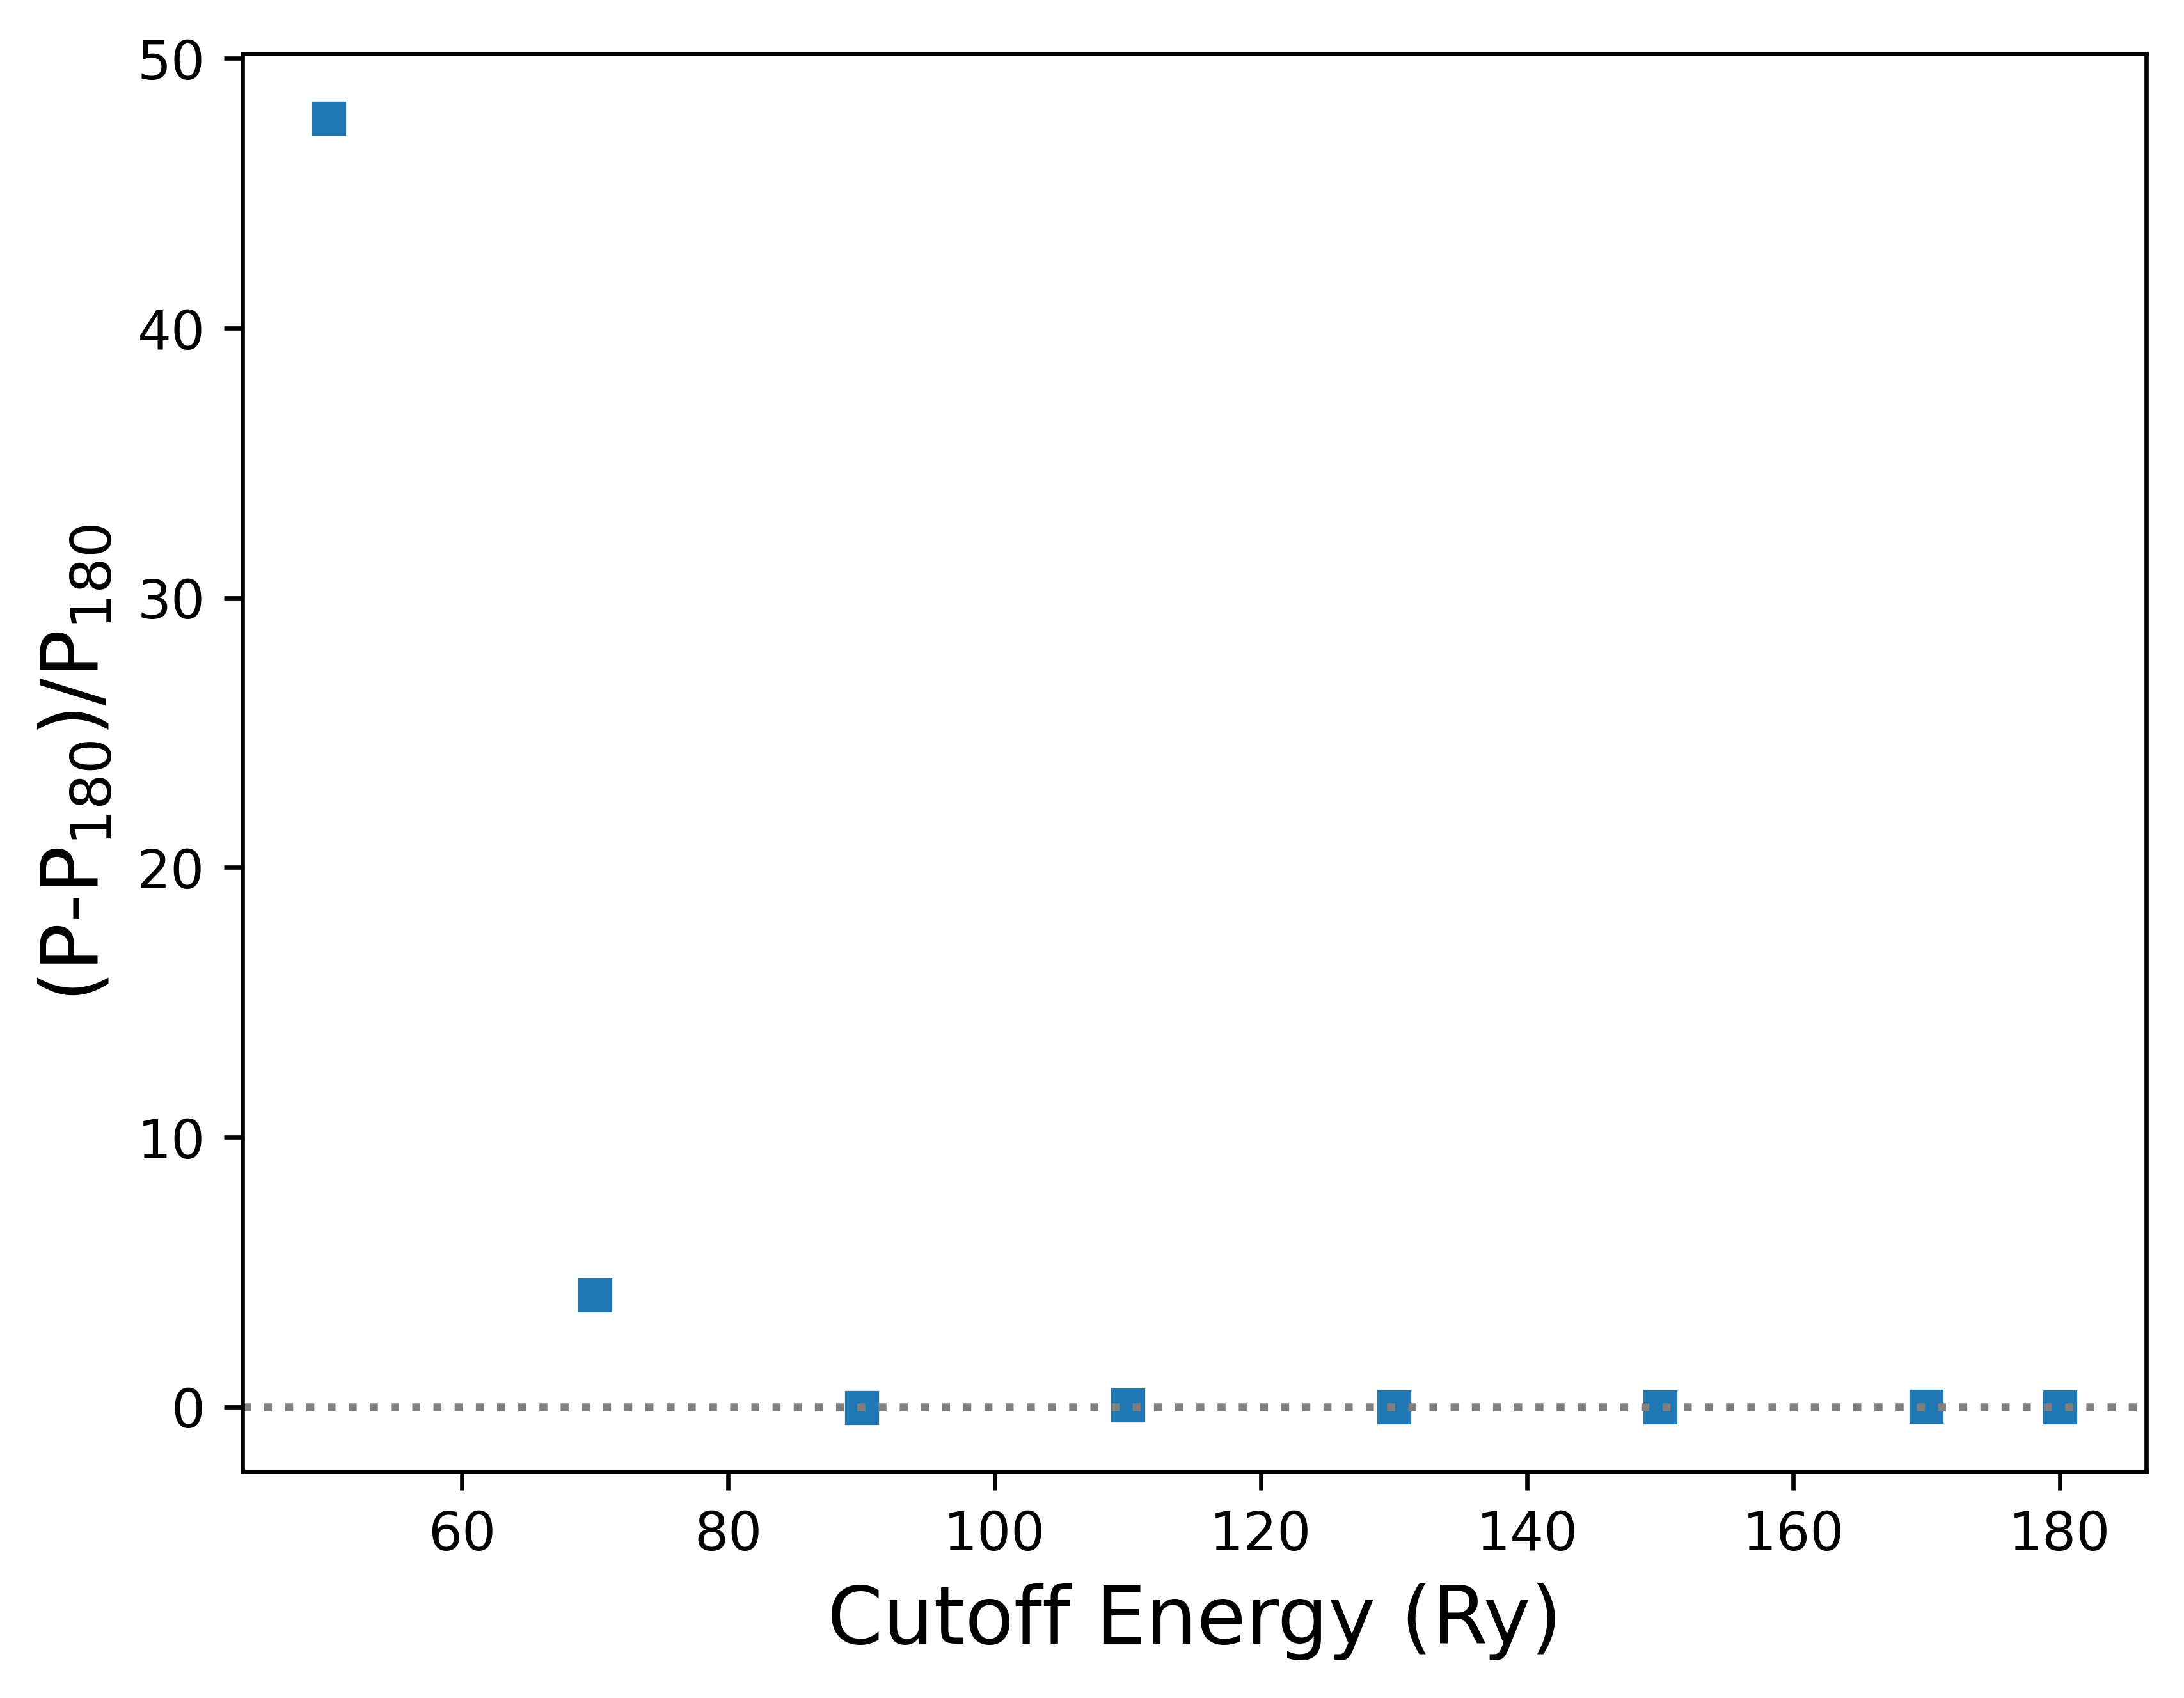
\includegraphics[width=1\textwidth]{convergence/R2SCAN/conv-pressure.png}
        \caption{}
        % \label{fig:}
    \end{subfigure}
    \caption{Convergence tests using the r$^2$SCAN functional on (a) total
        energy,
        (b) total force, and (c) total pressure.  All values are shifted
        with respect to the reference value at 180 Ry. The forces and pressure
        are also normalized with the corresponding reference values at 180 Ry.}
    \label{fig:conv_r2scan}
\end{figure}

\begin{figure}[h!]
    \centering
    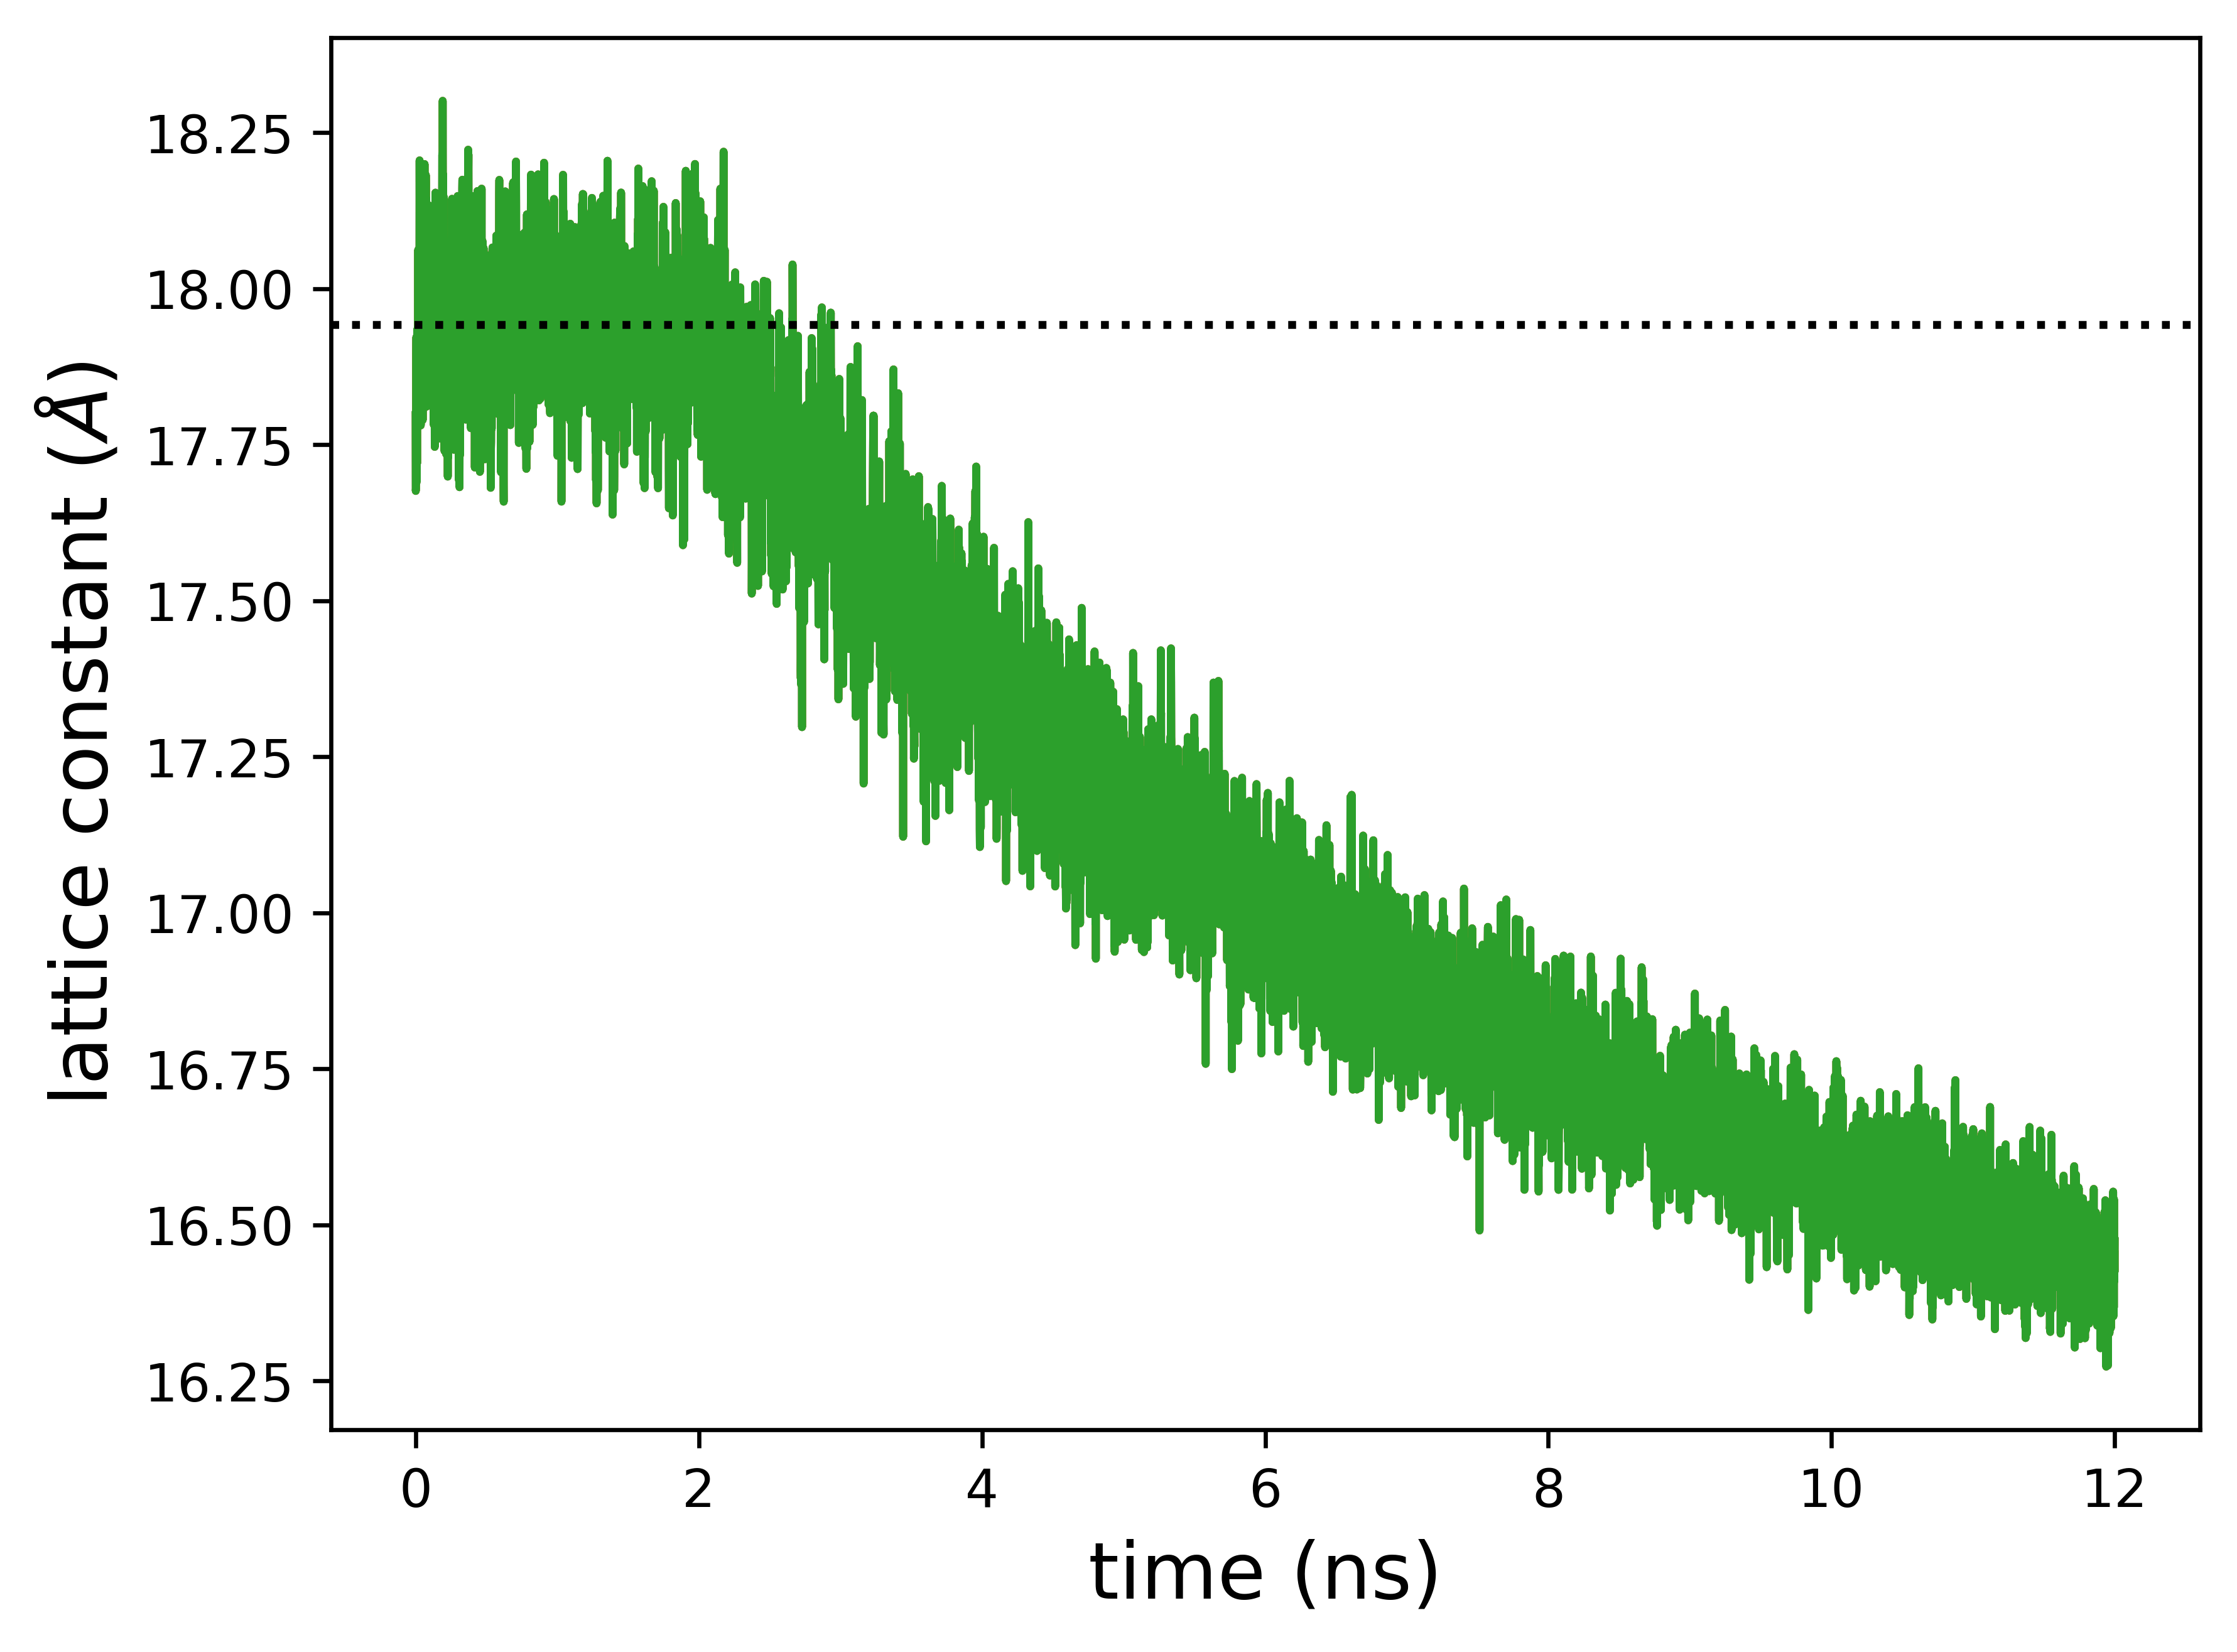
\includegraphics[width=0.4\linewidth]{images/330K/conv-lattice.png}
    \caption{Lattice parameter as a function of simulation steps. }
\end{figure}

\end{document}